\chapter{Интеллектуальных анализ данных Web-ресурсов}\label{ch:ch5}

\section{Анализ Web-графов}\label{sec:ch5/sect1}

\subsection{Beyond left and right: Real-world political polarization in twitter discussions on inter-ethnic conflicts}\label{subsec:ch5/sec1/sub1}

\subsubsection{1. Introduction}

Today, social polarization is believed to be growing both along traditional and newer lines along which schisms form \cite{DucaSaving}, of which political ones are, arguably, the sharpest. Despite the ever-increasing body of knowledge on political attitudes and alignments online, we still lack understanding of how political divisions show up in issue-oriented discussions and whether there is a cross-country pattern.

Despite all the well-described representation distortions \cite{Daniels}, the content of social media is still used for predicting consumer and/or electoral choices \cite{ColleoniRozzaArvidsson}, and the studies of political polarization on social media, including Twitter, are growing in popularity \cite{Barbera}. However, there are several shortcomings in today’s studies of political polarization in user-generated content.

Thus, in most cases, audience polarization is studied by examining purely political issues or events, while social conflicts of race, gender or religious origins with both evident and idiosyncratic polarization and politicisation \cite{McCrightDunlap} are rarely studied. Due to context and language differences, multi-country studies are also rare, especially where both established democracies and countries beyond the Euro-Atlantics are included, as, for most observers, these remain politically incomparable. However, conditions other than political regimes may create grounds for cross-cultural juxtapositions \cite{BodrunovaLitvinenkoBlekanov,BodrunovaBlekanovMaksimov}.

Another conceptual limitation is that, even in the most advanced studies, the detection of users’ political affiliations or ideologies is done via proxies, most often via structural network factors, such as: friendship affiliations; patterns of following \cite{BarberaJostNagler,Rivero}; or content sharing \cite{ColleoniRozzaArvidsson}, which could be misleading. Addressing this gap, newer works show that group polarization in social media may be studied by looking at user texts, including complex referrals to specific phenomena that matter for group identity \cite{Evolvi}. We argue that the analysis of political divisions needs to unite both structural and content aspects \cite{Bodrunova}.

In order to bridge these gaps in previous studies, we look at Twitter discussions regarding inter-ethnic clashes; they have similar conflict triggers and structure of social groups involved into conflict \cite{BodrunovaLitvinenkoBlekanov2017}. Whilst avoiding making straightfor- ward comparisons, we explore users’ political polariza- tion and suggest a mixed method to detect it across three cases in different political regimes: the USA; Germany; and Russia. By the UN estimates of 2013–2017, these countries have recently been the three most attractive countries to migrants in the world \cite{UN2013,UN2017} and have all witnessed violent inter-ethnic clashes that became global trending topics on Twitter.

This article, thus, is organized as follows: In Section 1, we review the approaches of assessing user polarization on social media and the conflicts under our scrutiny. In Section 2, we formulate the research questions and describe our methodology. In Section 3, we provide the results; in Section 4, we interpret and discuss them.

\subsubsection{2. Political Polarization on Twitter: The Current State of Research}

\paragraph{2.1. Political Polarization Studies and the Current Research Gaps}

Throughout recent years, mixed evidence has persisted in social media studies on whether users go online to agree or to argue \cite{YardiBoyd}. Research into echo chambers \cite{ColleoniRozzaArvidsson,Sunstein2002} has shown that user homophily, both structurally and semantically, may prevent the formation of online ‘opinion crossroads’, as there is ‘evidence of persistent ideological sorting in online communication networks’ \cite[p.~2]{Barbera}. However, a range of works point to the opposite effects in Twitter communication, with weaker ties responsible for the diversification of the consumption of political information \cite{Barbera} as well as different platform features on Twitter leading simultaneously to echo chambers and inter-community communication \cite{ConoverRatkiewiczFrancisco}. Thus, evidence suggests more research is needed to assess the patterns of users’ political clusterization on social networks.

Until today, most Twitter polarization studies are bound to the one-country-one-case strategy -- with a few notable exceptions \cite{Barbera,BarberaJostNagler}. Another problem arises from today’s understanding of online political polarization \cite{BramsonGrimSinger} as a situation when ‘a social or political group is divided into two opposing sub-groups having conflicting and contrasting positions, goals and viewpoints, with few individuals remaining neutral or holding an intermediate position’ \cite[p.~215]{CalaisGuerraMeiraJrCardie} \cite{Isenberg,Sunstein2002}.

Empirical evidence suggests that, if a heterogeneous group containing users with two opposing views has a non-zero cross-view retweet rate, it will end up as two polarized communities \cite{ConoverRatkiewiczFrancisco}. Following this logic, the studies of political polarization result in pre- defined binary descriptions of polarized communities -- see \cite{MoralesBorondoLosada} for Venezuela; 
\cite{AgathangelouKatakisRori} for Greece; or \cite{WeberGarimellaBatayneh} for Egypt.

However, for studies beyond the two-party electoral process, it seems useful to remember that polarization is an individual case of clusterization along schismatic lines, disregarding the number of resulting clusters \cite{EstebanRay}. In social conflicts, conflicting groups are not necessarily structured along binary political party divisions. The classic work of \cite{TajfelTurnerAustin} shows how social identity (including ethnic identity) divides in- and out-groups, while a later normative model of dissent in social groups \cite{Packer} implies that, in inter-ethnic conflicts, the majority may divide into pro- minority and anti-minority clusters if the anti-minority at- titude is perceived as harmful to the collective \cite[p.~5]{PackerChasteen}. Also, the very political spectra may be highly multi-dimensional, as The Manifesto Project (https://manifesto-project.wzb.eu/) or Polity Project (http://www.systemicpeace.org/polity/polity4.htm) suggest. Thus, we consider polarization more as multi-polar fragmentation of divergent clusters, of which bipolar clusterization is just an option.

Non-bipolar clusterization seems to be especially probable for ‘issue’ or ‘ad hoc’ publics \cite{BrunsBurgess,Papacharissi} that emerge on social networks. This claim is supported by research on the topic and issue-based discussions \cite{ElgesemSteskalDiakopoulos}. In single case studies, user polar- ization has been studied in regard to abortion, same-sex marriage, gun control, and climate change \cite{Elgesem,CalaisGuerraMeiraJrCardie,YardiBoyd}, with varying degrees and directions of polarization detected. Moreover, there is a clear difference in polarization patterns between political and non-political issues \cite{BarberaJostNagler}. But the evidence of differences in polarization patterns is still scarce in academic literature.

The biggest challenge in today’s polarization studies is that instead of taking into account the actual content of user posts, detection of users’ political affiliations is conducted via proxies. Of those, the most interesting results come from assessing structural network factors such as friendship affiliations \cite{BarberaRivero}, retweeting patterns \cite{CalaisGuerraVelosoMeiraJr}, patterns of political following \cite{BarberaJostNagler,Rivero} or content-sharing patterns \cite{AdamicGlance,BakshyMessingAdamic,ColleoniRozzaArvidsson,Elgesem}. However, using proxies may be misleading \cite{AdamicGlance} and even express analysis of actual tweets shows the extreme diversity of political views, both in the form of direct expression and in opinionated content.

However, if not proxies, then what? Several studies suggest that group polarization in social media may be examined by analysing complex user referrals to phenomena that matter for their identity and group alignment \cite{Evolvi}, as it is how the attitudes are expressed in natural language. In the simplest possible terms, one would take user attitudes (positive, negative, and neutral) towards particular objects for such referrals.

Thus, we will try to construct group divisions from the actual Tweet content by coding user referrals towards political players and then defining which of these attitudes divide the users most, and for how many clusters.

\paragraph{2.2. Lexicon-Based Approaches to the Analysis of User Polarization}

The area of research closest to our idea of bringing content into polarization studies is a lexicon-based analysis of Twitter data. In recent years, the field has experienced explosive growth, predominantly based on the analysis of sentiments. Without delving fully into these methodologies, we will simply note that the possibility of use of vocabulary-based approaches for polarization assessment tasks \cite{HillmanTrier} is usually based on combining lexical and structural analysis. Several researchers went beyond so-called ‘naïve’ sentiment and have tried to link affect \cite{StieglitzDangXuan} or appraisal \cite{DangXuanStieglitzWladarsch} in user texts, types of lexical units \cite{SperiosuSudanUpadhyay}, and structural elements of Twitter discussions, like graphs of following or speed and volume of Tweet dissemination. Using these and other works, one could conclude that a sentiment-based approach to detecting left and right differences would imply developing a ‘negative’ (say, leftist) + neutral + ‘positive’ (say, rightist) lexicon and applying them to the discussion bulk. However, the problem that we have run into with this approach is the following:

\begin{enumerate}
	\item The users expressed not ‘left views’ or ‘right views’ but attitudes (with their lexical markers) towards politicians, institutions, social groups, or events (‘actors’);
	\item A given user would express attitudes towards not just one but many actors of different political stances;
	\item The same user could express recognized- as-rightist attitudes towards one actor and recognized-as-leftist attitudes towards another actor of comparable significance (e.g., immigrants and nationalists);
	\item The same user could express negative views on both leftist and rightist actors (say, Barak Obama and the KKK in the USA).
\end{enumerate}

In case 3, the user’s preferences, as measured by one-dimensional positive/negative sentiment analysis, would create a zero-sum, and assigning the bias would not be possible. In case 4, an at least two-dimensional measurement of the political spectrum is needed. Taking this into consideration, we have further developed our research questions and the exploratory research design based on user sentiment, but not on pre-defined target-independent lexicons. Instead, to better capture user attitudes, we will use expert coding of Tweets, standardising the coding process with the help of the idea of ‘complex user referrals’ by Evolvi (2017) \cite{Evolvi}.

\paragraph{2.3. The Research Cases}

As stated above, we have studied three intergroup conflicts of ethnic or racial origins in the three leading immigration recipient countries: the USA, Germany, and Russia. Direct comparisons of ad hoc discussions \cite{BrunsBurgess} are currently viewed with some doubt in academic literature. Without developing a strictly com- parative research design, we have argued elsewhere \cite{BodrunovaLitvinenkoBlekanov2017,BodrunovaBlekanovMaksimov} that the conflicts we picked for the analysis are similar enough as research cases. They share a range of attributes: a violent interpersonal trigger, outbursts of public discussion across media platforms (becoming trending topics on Twitter), social polarization along the inter-ethnic or inter-race chasms, street action, and involvement of federal authorities. In addition, they were chosen because they were the first in a line of similar conflictual cases and, at least partly, set the communicative patterns for later discussions.

The cases are described as follows:
\begin{enumerate}
	\item A violent uprising against immigrants from Central Asia in the district of Biryulyovo, Moscow, Russia, in September 2013. After immigrant Orkhan Zeinalov, allegedly, killed local youngster Egor Scherbakov, the Biryolyovo residents destroyed the local warehouse and a trade centre around which hundreds of illegal immigrants had been dwelling. Several non-violent ‘people’s gatherings’ followed.
	
	\item Ferguson riots, Missouri, USA, in August 2014. There, unarmed African American teenager, Mike Brown was shot to death by white police officer Darren Wilson. The killing, as well as the defensive behaviour of the local police department, spurred several waves of street protests and peaceful support actions, including crowds at Mike Brown’s funeral ceremony.
	
	\item Mass harassment and rape of females on New Year’s Eve of 2016 in Cologne, Germany. Over 1,000 women reported being harassed during the celebrations on the city’s main square, allegedly, by re-settlers from North Africa and the Middle East. After that, demonstrations in protest were organized by radical political actors (PEGIDA movement and the party ‘Alternative for Germany’).
\end{enumerate}

\subsubsection{3. Research Questions and Methodology}

\paragraph{3.1. The Outline of the Research Design}

\paragraph{3.1.1. Research Questions} From what was said above, we have formulated the fol- lowing research questions:

\paragraph{RQ1. How, if at all, do the users cluster within the discussions, based on their attitudes to the major conflict actors? Does binary clusterization best describe user grouping?}

\paragraph{RQ2. Can the clusters be described as left or right in relation to the respective national political spectra? If not, then how could these clusters be described?}

\paragraph{RQ3. Are there similarities in the cluster structure of the discussions?}

\paragraph{3.1.2. The Research Design}

The way the RQs were formulated demanded an exploratory research design. To answer the research questions, we had to see which user groups emerged among the influencers and what discourses they conveyed.

Our concept for detecting user polarization was that political grouping within a discussion was constructed via a multi-dimensional combination of attitudes towards political actors (as defined above). These major political actors needed to be deduced from the discussions themselves. Then, the attitudes towards these players would be decrypted by expert coders for the key users, or influencers \cite{BodrunovaBlekanovMaksimov}, usually the bearers of the spectrum of attitudes.

The data received after coding would undergo clusterization, with each user belonging to one non-fuzzy cluster. Tweets by the users in the detected clusters would provide the word frequency vocabularies, which, after expert assessment, would turn into clusterization vocabularies. The latter would then be applied to all the users in the discussions, to see which users get into clusters and which discourses form there.

This approach, even if simple enough and reliant on expert intrusion, allows us to take into account the nature of the users’ political discussion, as well as the lack of linearity of their political positioning. We consider this crucial for studies on conflict discussions, as it may allow the inclusion of conflict-invoked (e.g., pro- or anti- minority), actor-oriented (e.g., authorities), and traditional political divisions (e.g., left and right and centre and radical). At this exploratory stage, our method does not imply machine learning or supervised approaches to data classification; we use big datasets at this stage of data collection only.

\paragraph{3.2. The Research Procedures}

\paragraph{3.2.1. Data Collection and Pre-Processing}

As this work is part of a bigger research project, our methods of data collection were described in detail previously \cite{BodrunovaLitvinenkoBlekanov2017}. Here, we briefly describe the steps we followed.

We used trendinalia.com to detect the initial discussion keywords and snowball reading to amplify this collection, thus forming the vocabularies for crawling. Trendinalia.com is a web service that allows daily monitoring of both world, regional, and national Twitter trending hashtags and words with no hashtag on an hourly basis, with the possibility of backdating; it has worked best in terms of detecting the trending topics, compared to the over ten other websites we had tried since 2013.

Using an API-independent Twitter crawler \cite{BlekanovSergeevMartynenko}, we collected the content of the discussions. All publicly available Tweets and the data on user interactions (likes, retweets, comments) were collected by a two-step procedure. Step one in- cluded the users who posted under the hashtags. Step two detected a wider community of likers, retweeters and commenters. On the discussion graph, only the step one nodes have been visualized.

Due to reasons regarding feasibility and sample comparability, collection periods differed. Thus, for Russia and Germany, the download period was 30 days after the trigger event. For the USA, we had to select the two weeks following the shooting, with Mike Brown’s funeral as the central event. The user samples included:

\begin{itemize}
	\item For Biryulyovo -- Step1: over 3,700 users; Step2: over 12,000 users;
	\item For Ferguson -- Step1: over 70,000 users; Step2: over 210,000 users;
	\item For Cologne -- Step1: over 12,000 users; Step2: over 99,000 users.
\end{itemize}

\paragraph{3.2.2. Data Analysis}

To answer RQ1, we needed to cluster key users by their political views, define the cluster vocabularies, and apply these vocabularies to the rest of the users, in order to see the discussion clusters and interpret their discourses.

As we expected the influencers to be bearers of the polarizing discourse, for each case, we defined the group of influencers based on nine parameters: the number of Tweets, likes, retweets, comments, in-degree, out- degree, degree, betweenness, and pagerank centralities. After these experiments, using various thresholds, the top 50 users were chosen as the cutting line for each parameter. As many users were repeated in the top due to several specifications, the duplicates were deleted. After elimination of influencers with low numbers of Tweets and bot-like influencers (with a percentage of repeated Tweets over 50\%) 156 users for Germany, 105 users for Russia, and 105 the USA were left. But, for the USA sample (which was several times bigger in the number of Tweets), the number of users was reduced by half, to 52 users. Their respective tweet collections for reading and coding included 13,359, 3,012, and 9,540 tweets.

To define user attitudes towards political actors, we developed scales for coding and coded the users (not their Tweets). The coders were experts in inter-ethnic conflict and, additionally, academic native-speakers, and the level of inter-coder reliability as measured by Cohen’s kappa reached at least 0.68 for any two sub-samples. The coders used the scale from \(-2\) to 2 to assess the attitude of each user to the following groups that had been identified as attitude triggers by reading the tweets before coding: 1) the minority (immigrants or African Americans); 2) ‘radical right’ or ‘radical white’ -- nationalists in Russia, PEGIDA and AFD in Germany, and the Tea Party and the KKK (as a label for radical whites) in the USA; 3) the incumbent country leaders -- Vladimir Putin and Dmitry Medvedev in Russia, Angela Merkel in Germany, and Barak Obama and Hillary Clinton in the USA; 4) local authorities and police forces grouped together as the ‘oppressive and responsible’ actors. Attitudes towards liberal opposition in Russia and to Republicans and Democrats were also coded, as we found them salient in the Tweets.

Based on this coding, the influences were clustered to form groups with similar combinations of attitudes. After clustering, the Tweets of each group were merged, and fully divergent frequency vocabularies of their discourses were formed with the use of expert vocabulary ‘cleaning’. Then, we applied the vocabularies to all the users in the discussions, to see how the discourses distribute within the discussion structure. We also measured whether these discourses formed distinct nebulae; but even if they did not, we assessed which users belonged to these discourses and interpreted the semantics of their speech qualitatively. What mattered for our analysis was whether the influencers formed distinct groups; all the following steps were the consequence.

In detail, the research steps were the following.

\begin{enumerate}
	\item Based on our coding, the influences of each case were grouped with the help of a k-means clustering algorithm with sorted the distances. With the number of clusters and the number of variables being diverse, the best solutions were finally chosen based on Silhouette metric S, within- and between-cluster square sums, examinations of variable means in each cluster (see Figures~\cref{fig:userAttitudesRussia} to~\cref{fig:userAttitudesUSA} for Russia, Germany, and the USA, respectively), and expert reading of tweets in each cluster. All the three influencer groups clustered well; Germany clustered best, Russia followed, and the USA the least, but all the solutions were sufficient by Silhouette from 2 to 10 possible clusters. To identify the best solutions, other aforementioned metrics were used. Those solutions were:
	\begin{itemize}
		\item For Russia: 4 variables (attitude to liberal opposition excluded), 3 clusters of 49, 36, and 20 users, \(S > 0.4\); 
		
		\item For Germany: 4 variables, 3 clusters of 99, 48, and 9 users, \(S > 0.5\);
		
		\item For the USA: 5 variables (attitude to Democrats excluded), 4 clusters of 15, 15, 12, and 10 users, \(S > 0.2\).
	\end{itemize}
	\item For each cluster, word frequency vocabularies were formed by merging the Tweets, ranging the words by frequency, and expert reading. After reading, only the words unique or highly characteristic for each cluster (for example, two mentions in one cluster and 160 in another would result into eliminating the word in the first one and leaving it in the other). If the difference between the numbers of mentions in any two clusters of the case was smaller than ten times, the word was eliminated in all the clusters.
	
	\item We applied the thesaurus to the rest of the users in each case; we wanted to identify the users who use the words from the divergent thesauri. As a result, we have received three types of users in each case: 1) the users who belonged to clusters 1 to 3 or 4; 2) the ‘overlappers’ who used the language of more than one cluster; 3) the users who did not use the discourses (mostly due to a low number of their Tweets). To ensure a higher quality of marking users, rather than using individual words from the thesauri, two-word combinations were used.
	
	\item Based on this information, we constructed the graphs of discourse distribution, with users as apexes and user interactions (comments and/or retweets) as edges, and calculated the indices for user centralities. We assessed who were the most influential discourse bearers and what they spoke about. We used Gephi algorithms OpenOrd and Force Atlas 2 for graph construction (see \cite{MartinBrownKlavans}, on OpenOrd), as the former favours centripetal graphing and the latter better shows visual homophily (see Figures~\cref{fig:openOrdRussia} to~\cref{fig:openOrdUSA}). To see whether the groups bearing the discourses were tighter than inter-group connections, we calculated the mean number of in-group and inter-group edges.
\end{enumerate}

\begin{figure}[ht]
	\centerfloat{
		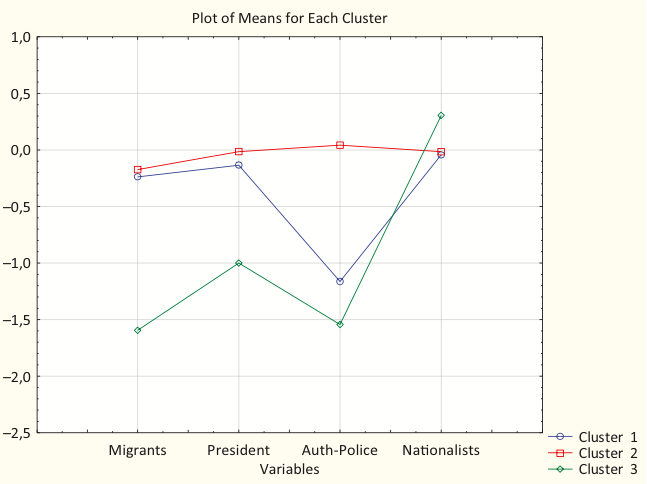
\includegraphics[scale=0.5]{userAttitudesRussia}
	}
	\caption{Mean values of user attitudes to the selected political actors in attitude-based clusters for Russia.}\label{fig:userAttitudesRussia}
\end{figure}

\begin{figure}[ht]
	\centerfloat{
		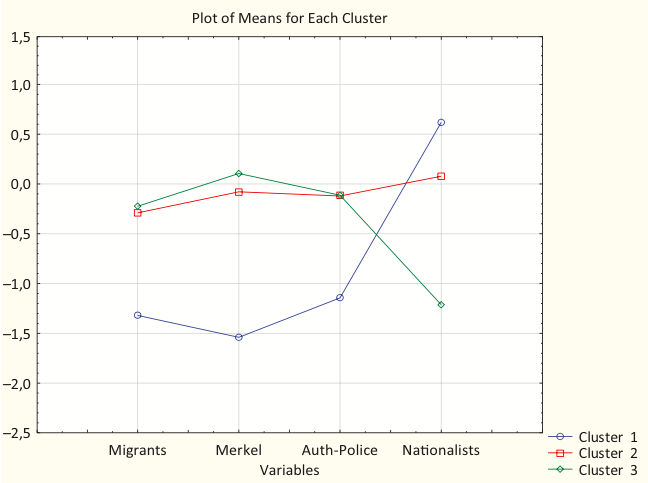
\includegraphics[scale=0.5]{userAttitudesGermany}
	}
	\caption{Mean values of user attitudes to the selected political actors in attitude-based clusters for Germany.}\label{fig:userAttitudesGermany}
\end{figure}

\begin{figure}[ht]
	\centerfloat{
		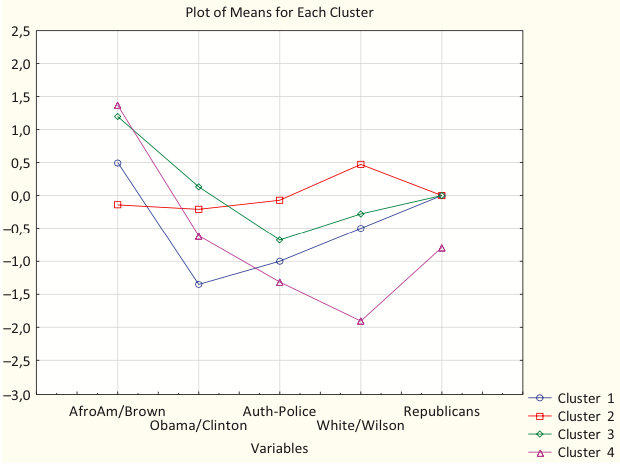
\includegraphics[scale=0.52]{userAttitudesUSA}
	}
	\caption{Mean values of user attitudes to the selected political actors in attitude-based clusters for the USA.}\label{fig:userAttitudesUSA}
\end{figure}

\begin{figure}[ht]
	\centerfloat{
		\hfill
		\subcaptionbox[List-of-Figures entry]{\label{fig:openOrdRussia-1}}{%
			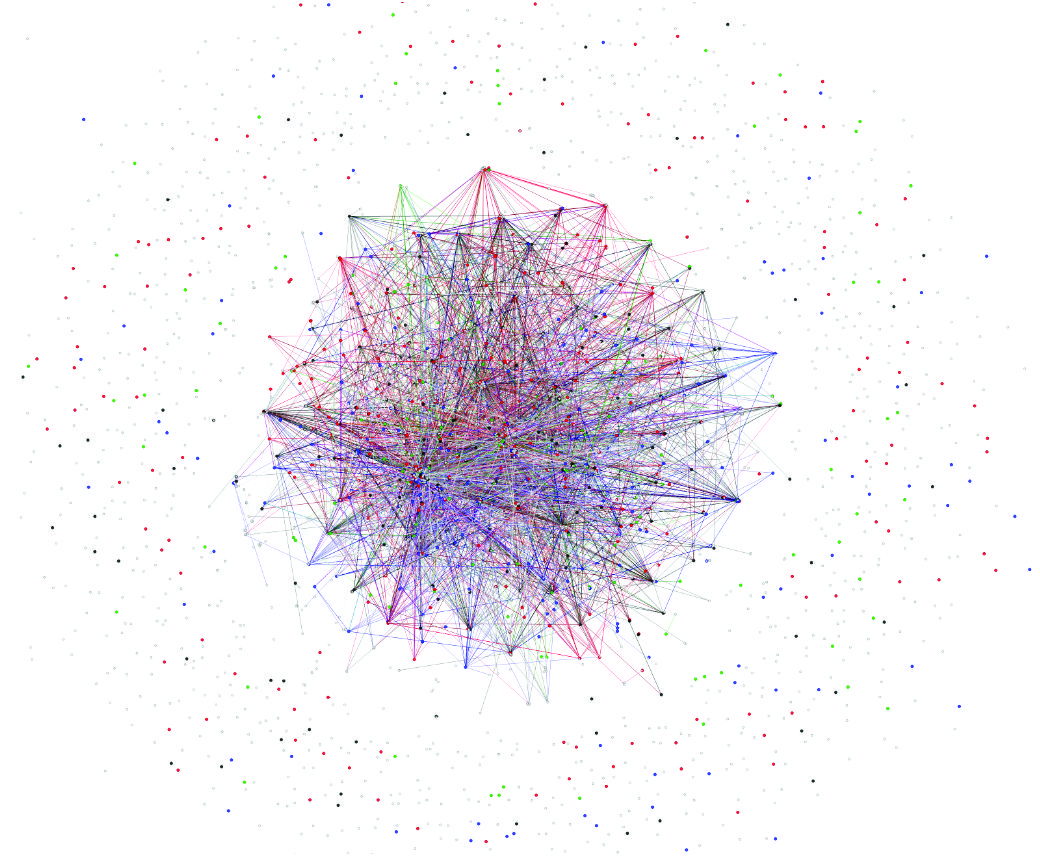
\includegraphics[width=0.419\linewidth]{openOrdRussia1}}
		\subcaptionbox{\label{fig:openOrdRussia-2}}{%
			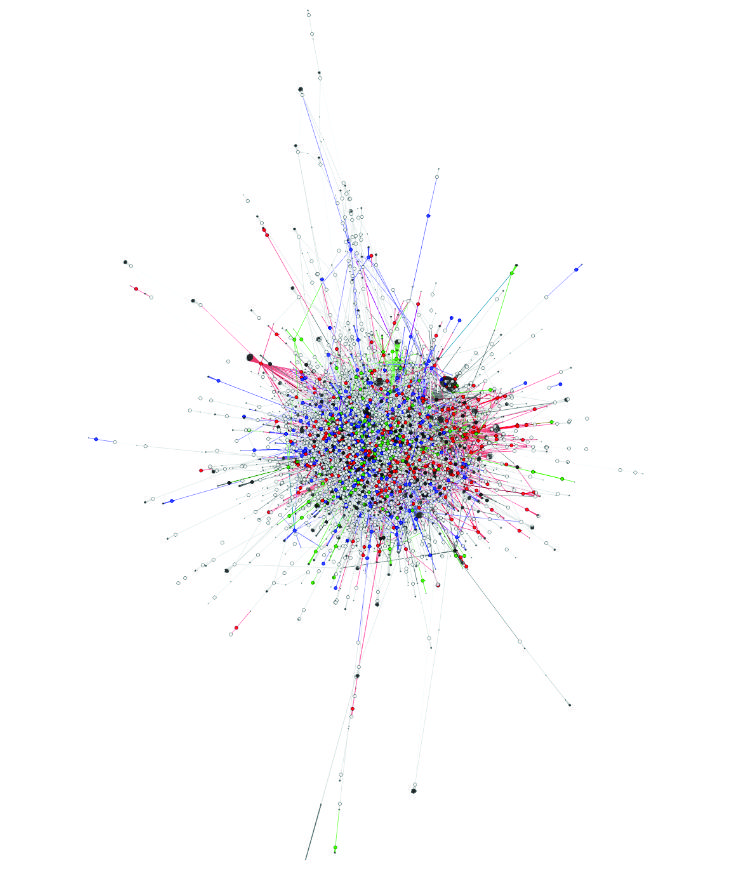
\includegraphics[width=0.4\linewidth]{openOrdRussia2}}
		\hfill
	}
	\legend{Blue: Cluster 1, ‘anti-establishment nationalists’; red: Cluster 2, ‘news disseminators’; green: Cluster 3, ‘angry citizens’; black: ‘overlappers’; grey: non-clustered users.}
	\caption{Communication within and between discursive groups of users in the discussions, with users as vertices and interactions (retweets and comments) as edges; reconstructed by OpenOrd and Force Atlas 2 algorithms for Russia.}\label{fig:openOrdRussia}
\end{figure}

\begin{figure}[ht]
	\centerfloat{
		\hfill
		\subcaptionbox[List-of-Figures entry]{\label{fig:openOrdGermany-1}}{%
			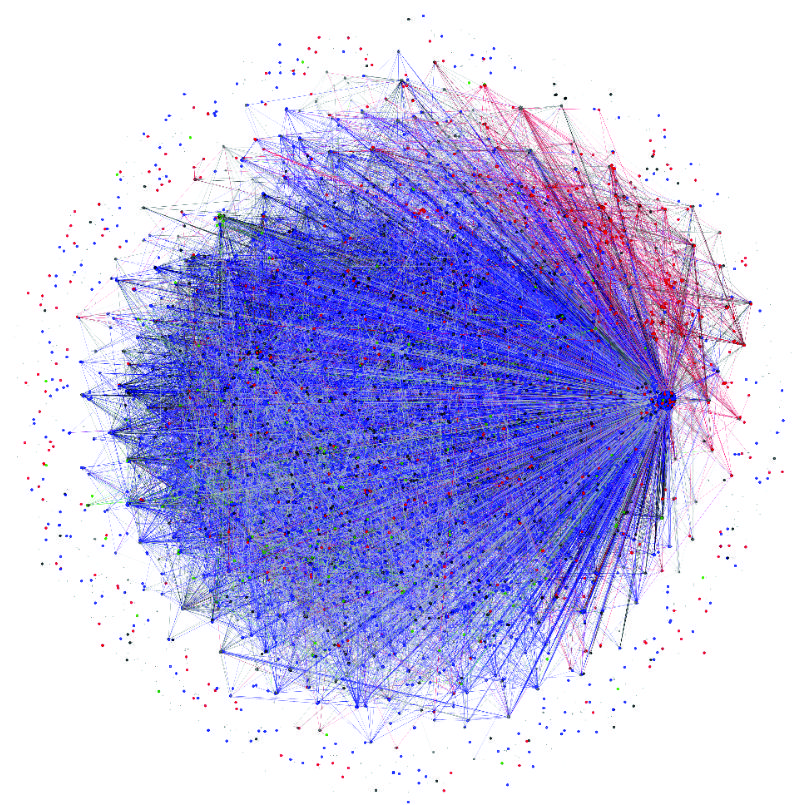
\includegraphics[width=0.419\linewidth]{openOrdGermany1}}
		\subcaptionbox{\label{fig:openOrdGermany-2}}{%
			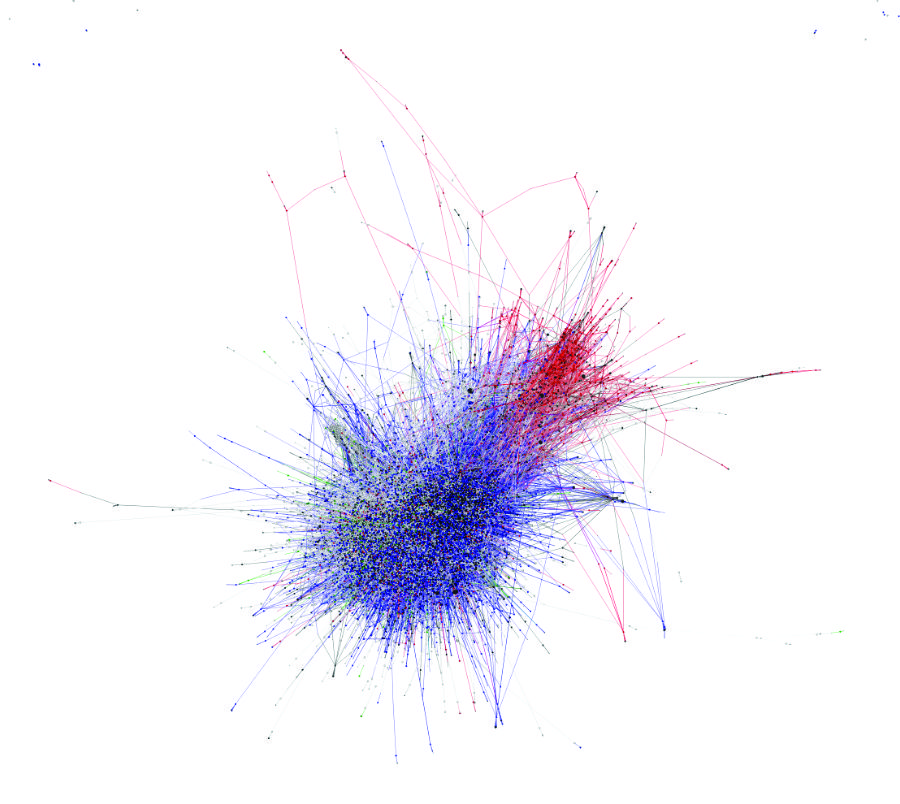
\includegraphics[width=0.4\linewidth]{openOrdGermany2}}
		\hfill
	}
	\legend{Blue: Cluster 1, ‘nationalists’; red: Cluster 2, ‘news disseminators’; green: Cluster 3, ‘anti-nationalists’; black: ‘overlappers’; grey: non-clustered users.}
	\caption{Communication within and between discursive groups of users in the discussions, with users as vertices and interactions (retweets and comments) as edges; reconstructed by OpenOrd and Force Atlas 2 algorithms for Germany.}\label{fig:openOrdGermany}
\end{figure}

\begin{figure}[ht]
	\centerfloat{
		\hfill
		\subcaptionbox[List-of-Figures entry]{\label{fig:openOrdUSA-1}}{%
			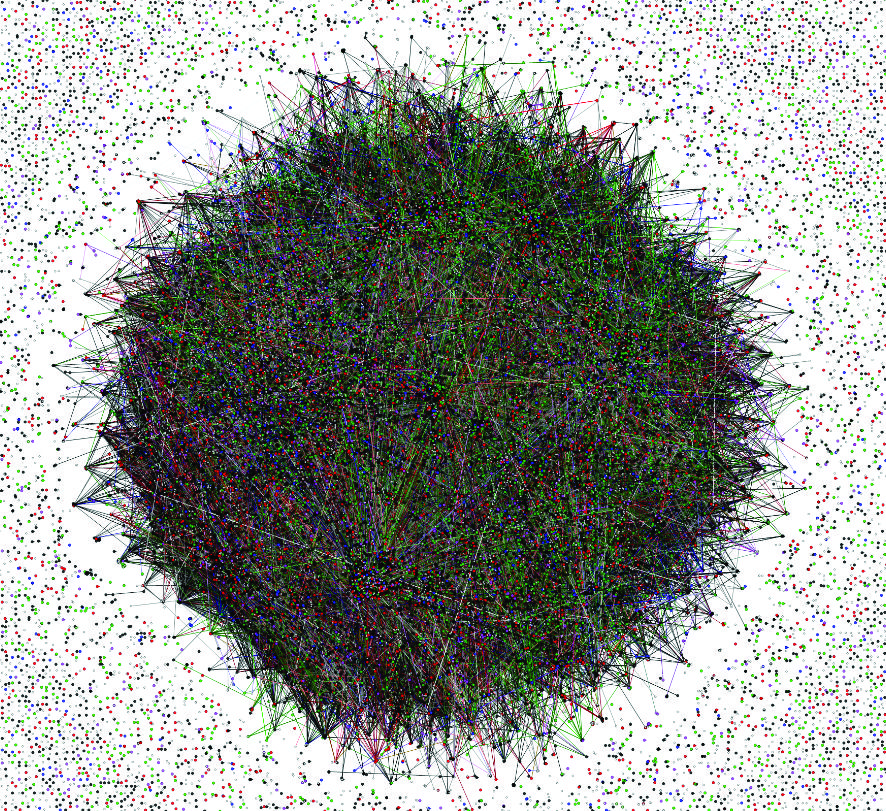
\includegraphics[width=0.419\linewidth]{openOrdUSA1}}
		\subcaptionbox{\label{fig:openOrdUSA-2}}{%
			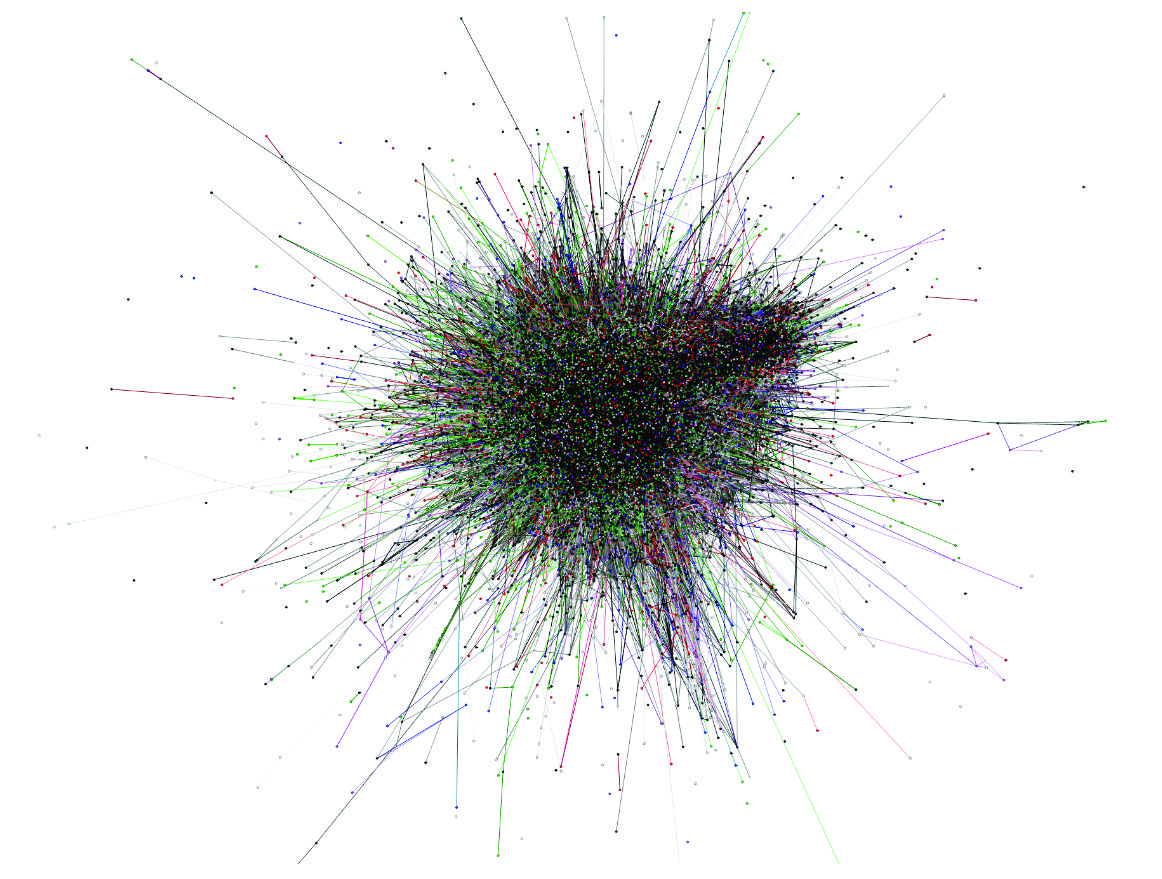
\includegraphics[width=0.4\linewidth]{openOrdUSA2}}
		\hfill
	}
	\legend{Blue: Cluster 1, ‘politicized observers’; red: Cluster 2, ‘media-oriented users’; green: Cluster 3, ‘human rights activists’; purple: Cluster 4, ‘whites’ blamers’; black: ‘overlappers’; grey: non-clustered users.}
	\caption{Communication within and between discursive groups of users in the discussions, with users as vertices and interactions (retweets and comments) as edges; reconstructed by OpenOrd and Force Atlas 2 algorithms for the USA.}\label{fig:openOrdUSA}
\end{figure}

To answer RQ2 about the left or right nature of the clusters, we partly recoded our coding data and corrected the graphs of means (Figures~\cref{fig:userAttitudesRussia} to~\cref{fig:userAttitudesUSA}) accordingly. Recoding was needed to re-interpret attitudes for and against a given actor as pro-left or pro-right. E.g., the influencers expressed attitudes towards political leaders (Obama, Merkel, and Putin), coded \(-2\) to 2. But, for the respective political spectra, Obama is leftist, while Merkel and Putin \cite{BluhmVarga} represent the rightist spectrum side. To ‘normalize’ the user attitudes, we recoded all the pro-left views as \(-1\) to \(-2\), and all pro-right views as 1 to 2 (see Table~\cref{tab:variableLeftRightNormalization}). By doing this, we could show on the graphs of means whether the clusters (and how many of them) were pro-left, pro-right, or mixed -- see Figures~\cref{fig:recordedDataRussia} to~\cref{fig:recordedDataUSA} for Russia, Germany, and the USA, respectively.

\begin{table}[ht]%
	\centering
	\caption{Recoding of variables for their left-right normalization.}%
	\label{tab:variableLeftRightNormalization}% label всегда желательно идти после caption
		\begin{adjustbox}{width=1\textwidth}
				\small
		\begin{tabular}{ c  c  c  c  c  c  c  c }% Вертикальные полосы не используются принципиально, как и лишние горизонтальные (допускается по ГОСТ 2.105 пункт 4.4.5) % @{} позволяет прижиматься к краям
			\toprule
			Country & Minority & President & Police-Authorities & Nationalists & Opposition & Democrats & Republicans\\
			\hline
			Russia & Recoded & Not & Not & Not & Recoded & -- & --\\
			Germany & Recoded & Not & Not & Not & -- & -- & -- \\
			USA & Recoded & Recoded & Not & Not & -- & Recoded & Not \\
			\bottomrule
		\end{tabular}%
			\end{adjustbox}
\end{table}

\begin{figure}[ht]
	\centerfloat{
		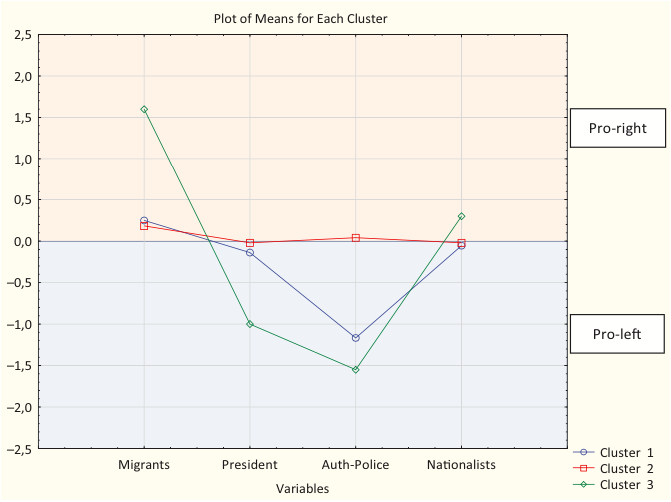
\includegraphics[scale=0.5]{recordedDataRussia}
	}
	\caption{Mean values for the recoded data on user attitudes towards the selected political actors for Russia.}\label{fig:recordedDataRussia}
\end{figure}

\begin{figure}[ht]
	\centerfloat{
		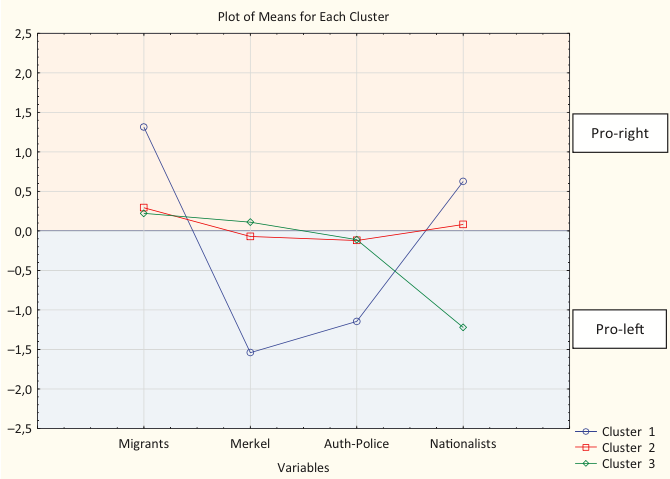
\includegraphics[scale=0.5]{recordedDataGermany}
	}
	\caption{Mean values for the recoded data on user attitudes towards the selected political actors for Germany.}\label{fig:recordedDataGermany}
\end{figure}

\begin{figure}[ht]
	\centerfloat{
		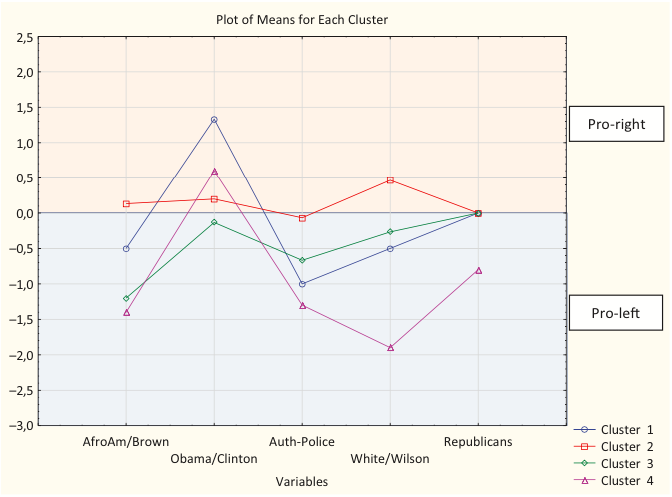
\includegraphics[scale=0.5]{recordedDataUSA}
	}
	\caption{Mean values for the recoded data on user attitudes towards the selected political actors for the USA.}\label{fig:recordedDataUSA}
\end{figure}

To answer RQ3, we qualitatively assessed the results for RQ1 and RQ2.

\subsubsection{4. Results}

Our results show that the discourses identified by coding influencers cover a substantial part of the discourse in all the cases: for Russia, the thesauri covered 31,5\%, in Germany, 63,4\% and, in the USA, 73,5\% of the users. This shows that influencers’ talk reflects the discourse of ‘ordinary users’ to different extents in each country, but everywhere we were able to detect the discourses that were important for the overall discussion.

As the figures suggest, in all the three cases, group structure was not binary; moreover, binary solutions for each country would hide important discourses that actually constituted the discussions. Neither did the group divisions correspond to the minority/pro-minority majority/anti-minority majority scheme. Instead, the clusters may be described as follows:

For Russia, the clusters include: ‘news disseminators’; ‘anti-establishment nationalists’; and ‘angry citizens’. The first group was mostly neutral but formed a substantial part of the political discussions by supplying (posting or retweeting) news at each stage of the conflict. The second cluster was clearly anti-immigrant and nationalistic but differed from European nationalism. Within the discussion, there was also an evident divide between the nationalist groups who supported the current establishment and those who actively opposed it. The former saw the incumbent leadership as the flesh of the 1990s’ elites who ‘had stolen the country’; such users, therefore, blamed the national policymakers for supporting the post-Soviet immigration. The second type of nationalism -- the pro-establishment one -- showed up in the third cluster of ‘angry citizens’. This cluster united anti-institutionalists who were raising voices against \textit{bespredel} (‘the absence of limits’ and rules of the game), but in differing ways. This diverse group included pro-Putin nationalists who were ready to fight with the Moscow riot police, liberal oppositional media and public figures who criticized the policymakers, and ‘tired citizens’ who negatively treated the immigrants, and the country leaders, and the local authorities, and the nationalists. Unlike in the ‘news disseminators’ cluster, the close-to-zero means for these variables here were the result of pro- and anti-establishment views compensating each other while the users united against police (see Figure~\cref{fig:userAttitudesRussia}).

For Germany, the clusters include: ‘news disseminators’; ‘nationalists’; and ‘anti-nationalists’. Discursively, the biggest group of ‘nationalists’ unites two similar sub-groups, one with slightly more aggressive tendencies towards small liberal-oriented parties and activist movements (like Antifa), and the other more critical of the national government. The anti-nationalist group is, however, also salient, making the German picture one-dimensional in terms of political divisions (pro- and anti-minority), even if the dimension is not political-party but issue-based. Also, the overlappers play a significant role here, as they visually stand in between the two opposing clusters, thus creating bridges for public dialogue (see Figure~\cref{fig:openOrdGermany}).

For the USA, the clusters include: ‘media-oriented users’; ‘human rights activists’; ‘politicized observers’; and ‘whites’ blamers’ (see Figure~\cref{fig:userAttitudesUSA}). Within the influencers, the clusters were similar in volume, but, on the big graph, the last two groups were relatively small- scale, while the first two dominated the graph. Just as in Russia, the media-oriented discourse was a part of the political discussion, but the three other groups were not neutral, especially ‘whites’ blamers’ and ‘human rights activists.’ The former actively blamed ‘the white dominance’ and called for action against oppression. Interestingly, the hashtag \#blacklivesmatter was less important for this group than for the media-oriented discourse. However, blaming hashtags and words like ‘murderer,’ ‘republikkklan,’ or ‘kkkop,’ and calls for action (like ‘\#arrestdarrenwilson,’ ‘\#boycottgofundme,’ or ‘\#donotshopmonday’), were prominent. The other group, very different from ‘whites’ haters,’ and linked the case to human rights issues like abortion (\#prolife), gender inequality (\#womeninequalityday), morality (\#moralmonday), and others. The group itself, as one can see even from the hashtags, was polar in itself in terms of left and right divisions on human rights. For this group, positioning on Mike Brown’s death was different, expressed mostly by ‘don’t shoot’ hashtags. ‘Politicized observers’ abstained from taking clear sides, but discussed the Ferguson events in terms of its influence upon the political process in America. Interestingly, the cluster that mostly reposted media, was the most pro-Wilson, as media, evidently, tried to remain balanced; they also reported police press conferences that were modestly defensive towards Darren Wilson.

Then, we looked at how the discourses we described spread inside the graph. Our task was not to calculate the level of homophily and prove user clustering for all the discussions; the goal was to see how the discourses actually spread and whether they spread in a similar way -- and they did not. For Russia and the USA, the discourses mixed, but if in Russia we saw inter-cluster talk, in the USA overlappers took almost all the space in the graph centre. And in Germany, the graph was clearly structurally divided. This was also proved by the mean in- and inter-cluster weighted number of edges: in Russia, the inter-cluster links took over (216 vs. 323.5, respectively), while in Germany (4392.75 vs. 2890.25) and the USA (21114.4 vs. 3755.2) in-group connections were stronger.

Thus, the attitude-based grouping was different in each of the three cases. Also, it was far from clear left-right identifications. In order to show it, we have recoded the variables as stated above, making pro- left views negative (\(-1\) to \(-2\)) and pro-right views positive (1 to 2). We considered anti-minority, anti-Obama/Clinton, pro-Putin/Medvedev, pro-Merkel, pro-police, pro-nationalist, anti-opposition (in Russia), anti-Democrat, and pro-Republican (in the USA) views pro-right, while the opposite was marked pro-left. See the full recoding scheme in Table~\cref{tab:variableLeftRightNormalization}.

The resulting graphs of means are quite telling (see Figures~\cref{fig:recordedDataRussia} to~\cref{fig:recordedDataUSA}). Both in Russia and Germany, the leaders representing rightist sides of the spectra have actually taken pro-migration stance, and this has made right-wing users who support nationalist movements and speak against immigrants, move left and be against the incumbent leaders, as well as against the local authorities and police for ‘not protecting’ the host communities. But the other clusters in the two countries quite strongly differ from each other. While in Germany issue-based leftism is clearly seen, the other Russian cluster of ‘angry citizens’ diverges into three discourses that combine clearly rightist, pro-establishment nationalism; liberal, anti-establishment oppositional speakers; and politicised citizens. These politicised citizens, paradoxically for external observers, do not support any of the existing political factions, due to their impotence in resolving local problems. Thus, at least two nationalist discourses were detected by us for Russia -- while in the USA there are two very different left-wing clusters, one clearly left, supportive of either Obama or Clinton and based on human rights’ discourse, and another that was sharply anti-white, even blaming Obama for not being protective enough, which, in our rough coding, made the cluster stick out to anti-Obama views on the rightist side of Figure~\cref{fig:recordedDataUSA} (in effect, being extreme left). The cluster of ‘politicized observers’, interestingly, is reminiscent of the ‘tired citizens’ in Russia, as they are, on average, only slightly pro-African-American and, more strongly, anti- leader, anti-police, and anti-majority.

Another crucial observation is that, while the divisions in the discussion clearly stem from local political contexts, they are quite far from expectations determined by the systemic political features of the countries. Thus, in the majoritarian USA where one would expect two-sided polarization, the clusters were, in fact, numerous and the discussion was based on overlappers. It was rather coalitional Germany that showed polarization. And in Russia, just one side of the spectrum was present in the discussion. Thus, it is not only the local political markets but also the nature of the issue and issue-based divisions that shape political clustering
.
Overall conclusions are thus the following: The discursive schisms do exist in issue-based discussions, but they do not fall into binary categories according to majoritarian political divisions, and; they only partially fall into the three-side divisions expected by the nature of the issue. Instead, local political spectra may provoke the formation of, for example, two leftist or two rightist clusters. Only Germany has demonstrated the expected divisions between anti- and pro-minority majority, while the minority remained highly under-represented at all, like in Russia -- and unlike in America.

The similarities can also be traced, but not in terms of left and right divisions. First, in all the discussions, a politically neutral news-based cluster played a significant structural role. Second, all three discussions revealed harsh anti-institutionalism, including that from the users who, in conventional logic, were expected to support the incumbents. Third, Germany and Russia were similar in how nationalist clusters were against the conservative governments, and Russia and the USA were similar in how the ‘tired citizens’ were politicised against all the political sides.

\subsubsection{5. Conclusion}

In our article, we have combined content analysis of social media with cluster analysis and graph construction. Our method has revealed greater complexity of politicised discourse within ad hoc Twitter discussions on inter-ethnic conflicts. Thus, we have found that there may be several clusters of leftist or rightist views even if the number of clusters is minimal, and users may combine formally leftist and rightist views if positions of political actors or the nature of the issue demand it. The groups we have detected differ highly in their conceptualisation from the traditional left and right divisions and left or right labels cannot be attached to individual users based on their preferences, like pro- and anti-minority stances or treatments of country leaders or parties. We have also shown that, on the graphs, the discourses intertwine quite intensely if we do not force the graphs to artificially diverge according to users’ political views.

Our research provides new input for rethinking the political divisions that form online, on what grounds they form, and how to detect them. The local political contexts, as well as the nature of the issues under scrutiny, are major factors to be taken into account. In our article, the ‘issue publics’ provide clues on how political opinion is veering away from traditional left and right divisions, and Twitter communication is more complicated than the imaginary cocooned talk in echo chambers, especially for issues beyond elections and direct policing.

Limitations of our method stem from the subjectivity of coding and from the low number of coded influencers, but these may be partially overcome by automatisation of coding collections and the increase of the number of coded users thanks to automatisation. Our method may be applied to detect hidden issue-oriented polarization beyond one-dimensional left-right political spectra.

\subsection{Please Follow Us: Media roles in Twitter discussions in the United States, Germany, France, and Russia}\label{subsec:ch5/sec1/sub2}

\subsection{Multi-dimensional echo chambers: Language and sentiment structure of Twitter discussions on the Charlie Hebdo case}\label{subsec:ch5/sec1/sub3}

\subsubsection{1. Introduction}

Public discussions on social networks potentially have trans-border and multilingual nature. This comes true in heated conflictual discussions that reach global trending topics. Such discussions are expected to demonstrate ‘civilizational clashes’ \cite{AnKwakMejova}.

Being part of the global public sphere, since the 1990s, such discussions were expected by many observers to be more horizontal, all-involving, and democratically efficient \cite{Fuchs} than the traditional mass-mediated discussions \cite{McQuail}. But, with time, criticism towards the democratic quality of discussions in social media arose, with many works discovering the patterns of echo chambering and discourse polarization in social networks \cite{Sunstein2001,Sunstein2002,BarberaJostNagler,BastosMerceaBaronchelli,ColleoniRozzaArvidsson,ConoverRatkiewiczFrancisco}, which lowered the capacities of inter-group discussions and, thus, just formed an additional line of social segregation.

Object-oriented hashtagged discussions have been thoroughly studied in the 2010s, including those on political and social conflicts. But there is still scarce knowledge on whether affective hashtags \cite{Papacharissi} that convey emotions -- either of solidarity with or of anger towards a particular social group -- work in terms of user clusterization. Also, there is no clear understanding of comparative democratic quality of emotionally ‘positive’ and ‘negative’ hashtags in terms of echo chambering.

In this paper, we address these gaps by analyzing the Twitter discussion on the \textit{Charlie Hebdo} massacre of 2015. In the discussion upon the mass killings, the Twittershpere has created \#jesuischarlie and \#jenesuispascharlie -- two emotionally differing discussion clusters with, allegedly, opposite sentiments towards the journal’s ethics and freedom of speech; the hashtags soon became ‘role models’ for online solidarity towards the victims of terrorist attacks and anthropogenic disasters.

To analyze the echo chambering patterns in the two discussions, we have focused upon two levels of echo chambers. We were wondering whether echo chambers formed on the level of a hashtag (based on language use) and within a particular language (based on user sentiment of French-speaking users).
The remainder of the paper is organized as follows. Section 2 reviews the literature on echo chambering in social media. Section 3 presents our methodology and the conduct of the research. Section 4 presents our results and discusses them.

\subsubsection{2. User Groupings on Twitter and the Efficacy of Public Sphere}

\paragraph{2.1 Social Media and the Public Sphere: Echo Chambers vs. Opinion Crossroads}
Public sphere as a spatial metaphor for a complex of discussions and procedures with a public status and decision-making goals \cite{Kleinstuber} has been amplified by the appearance of social media in the 2000s. By 1990s, it had been established in the academic literature that mediatized public sphere with traditional media playing the role of information hubs was uneven and hardly efficient in terms of access to opinion expression, as whole social groups remained under-represented, and newsmakers privileged in comparison to \textit{vox populi}. With the appearance of social media, hopes arose that the new communicative milieus would foster horizontalization of communication and provide for democratization and higher political participation \cite{Fuchs}. Also, hopes for better understanding and resolution of non-political inter-group conflicts existed.

But with time, these hopes fainted, as offline disparities seemed to reproduce online, including political interests, race, gender, and other inequalities \cite{Daniels}; emotion and affect proved to rule the discourse \cite{Papacharissi}, with publics even in most democratically developed countries moving from diverse in opinion to dissonant and disconnected \cite{Pfetsch}. With the development of social network analysis (SNA) and its application to social media research, the question of the efficacy of the public discussions in social media \cite{BrunsHighfield} became linked to network and structural features of the discussions, such as the influencer status \cite{BodrunovaBlekanovMaksimov,BodrunovaLitvinenkoBlekanov2016} and clusterization of users also known as user polarization \cite{BarberaJostNagler,BastosMerceaBaronchelli} and echo chambering \cite{ColleoniRozzaArvidsson,ConoverRatkiewiczFrancisco}. Some evidence was also gathered on discussion sphericules forming on the global scale just as well as nationally \cite{CammaertsAudenhove}.

\paragraph{2.2 Why the Twitter Discussions Fragment: Linguistic Properties of Speech as Catalyzers of Echo Chambering}
In early studies of social networks and its users, authors interested in testing the ability of networks to pull together users from distant locations and weak ties linked geo- graphical distance with factors like residence of users and their language profile \cite{TakhteyevGruzdWellman}. This is why Twitter that enabled the (arguably) quickest possible information spread across locations and languages became a major attractor of scholarly attention \cite{LotanGraeffAnanny,HongConvertinoChi}. But despite the global reach of the platform, several studies have found that people were still connected locally on Twitter \cite{CammaertsAudenhove,YardiBoyd}.

Along with locality and residence, linguistic factors, arguably, play a major role in user grouping on the global scale. Thus, the language(s) used by the discussion participants is the first natural barrier that is expected to make users group together and communicate within their language-based echo chambers \cite{ChenTuZheng}, both on Twitter on the whole and within particular hashtags \cite{BastosPuschmannTravitzki}.

Other factors have also been discussed as the catalyzers of user grouping on Twitter. Among those, political attitudes lead the research agenda \cite{BarberaJostNagler,BastosMerceaBaronchelli}. Here, several ways to detect user clusterization exist. Of them, use of network or semantic proxies like friendship ties \cite{BarberaRivero}, patterns of following \cite{Rivero} and retweeting \cite{CalaisGuerraMeiraJrCardie}, content sharing \cite{ColleoniRozzaArvidsson,BakshyMessingAdamic} etc. is till today the most prominent; another is automated analysis of user sentiment, either in general or toward an issue/actor in question (object-oriented) \cite{ConoverGoncalvesRatkiewicz}.

But all these studies depict user groupings within a single dimension; our idea is to try and trace user groupings multi-dimensionally -- both on the level of a hashtag (based on language use) and within a language nebula (based on user sentiment).

\paragraph{2.3 The \textit{Charlie Hebdo} Case: Emotional Hashtags and User Groupings}
To search for multi-dimensional echo chambers, we have chosen the case of the \textit{Charlie Hebdo} massacre of 2015. Here, we could hypothesize that the existence of emotionally opposite hashtags (\#jesuischarlie and \#jenesuispascharlie) already creates enclaves within the general discussion on the case. Then, within the hashtags, several clusters based on language structure may exist. Then, on the third level, we will look whether within the language clusters sub-clusters of sentiment form. In general, our idea is to see how exactly the language clusters correspond to the sentiment clusters in each language and whether ‘positive’ users within one language are linked to such in another language, while ‘negative’ users also group across languages in a similar way. But here we present only preliminary results that check if the user clusters may at all be detected based on language and on sentiment within a language.

\paragraph{2.4 Research Hypotheses}

Thus, our hypotheses are the following:
\begin{itemize}
	\item H1a. Non-random user groups will be detected for both hashtags, as based on
	language use.
	\item H1b. \#jesuischarie will not differ from \#jenesuispascharlie in their language
	structure, as both hashtags have reached global trending topics and are expected to show ‘civilizational clashes’.
	\item H2a. Non-random user groups will be detected within one language (French), as based on positive and negative sentiment.
	\item H2b. \#jesuischarlie will differ from \#jenesuispascharlie in the grouping based on user sentiment, due to the emotional opposition of the hashtags themselves.
	\item H3. Multi-layer echo chambering may be detected in trans-border hashtagged discussions of global reach.
\end{itemize}

\subsubsection{3. Data Collection and Conduct of Research}

\paragraph{3.1 Data Collection and the Datasets}
Using a web crawler developed especially for the Twitter data collection, we gathered all the tweets published openly under the hashtags \#jesuischarlie and \#jenesuispascharlie (by separate crawls) within January 7 to 9, 2015, as these three days covered the active conflict (from the killings in the editorial office to the assailants’ death) when the users provided virtually millions of tweets for collection.

The collected datasets included: for \#jesuischarlie: 420,080 tweets; 266,904 tweeters; 719,503 users who interacted with the posted tweets (by likes, retweets, or comments); for \#jenesuispascharlie: 7,698 tweets; 5,466 tweeters; 17,872 users who posted and interacted with the posted tweets (by likes, retweets, or comments).

These full datasets were later used to reconstruct the overall web graphs for the two hashtags. But the datasets were very different in size, and be able to color them with language markers, we needed to sample the users for coding having in mind the volume difference of the datasets.

\paragraph{3.2 Language Analysis: Sampling, Coding, and Graph Reconstruction} 
To answer H1a and H1b, we have coded the users for their language use and then applied these data to the datasets for web graph reconstruction.

After eliminating bots and bot-like users (those who posted over 60\% of doubled tweets) as well as hashtag-only tweets, we have followed the strategy developed by the research group for previous Twitter studies \cite{Authors2016a,Authors2016b,Authors2018}, namely uniting random sampling with detection of influential users (influencers) for taking them into account. Then, we have coded all the influencers (disregarding the number of tweets they posted; for \#jesuiuscharlie, 402 users, for \#jenesuispascharlie, 85 users) and ‘ordinary users’ sampled in the feasible and comparable way. For \#jenesuispascharlie that was substantially smaller, all the users with 3 and more tweets were coded (339 users); for \#jesuischarlie, the ‘ordinary users’ with 5 tweets or more were taken into account (9,090 users), and of them, each second was coded (4500 users).

All the sampled underwent expert reading and were coded manually marking the number of tweets in language 1, language 2, and other languages; thus, users posting on one, two, and three or more languages were defined. The languages were identified for each user; in case of rare languages, Yandex language identifier was employed.

To reconstruct the graphs, we use Gephi API algorithms openly available online. Of the available algorithms, two were chosen: Hu \cite{Hu} and OpenOrd \cite{MartinBrownKlavans}; here, YifanHu-based graphs are presented, as the OpenOrd graphs require more space for presentation. We colored both the nodes (users) and the edges (connections between users). To prove that the visual nebulae are not artifacts of subjective viewership, we calculated the percentage of edges between and inside language groups, eliminating the ‘loops’ of self-commenting/liking by the users.

\paragraph{3.3 Sentiment Analysis: Sampling, Vocabulary Building, and Graph Reconstruction}After we have proved that the French-speaking users show non-random grouping in both cases (see below), we have taken them for sentiment analysis. The number of users for \#jesuischarlie included 1291 user; for \#jenesuispascharlie, 117 users.

Our strategy for French-language sentiment analysis was the following. We have united three sources in our vocabulary: the existing French dictionary with sentiment marking, machine translation from an additional Wordnet vocabulary, and the case-based vocabulary created from the collected tweets and manually marked for positive, negative, and neutral sentiment regardless of the case-specific meanings.

This vocabulary was applied to each tweet of the abovementioned French-speaking users; for each tweet, the sentiment was calculated. Then, the thresholds were defined: positive and negative were the users with positive(+neutral) and negative(+neutral) tweets, respectively; neutral were those with neutral tweets only; mixed were those with positive + negative(+neutral) tweets.

Then, we also checked the groupings with by calculating the percentage of edges both between and inside language groups, eliminating the ‘loops’ of self-commenting/liking by the users.

\subsubsection{4. Results and Discussion}

Our results are described below with regard to the hypotheses stated above.

\textit{H1a/H1b.} To assess the user groupings in both hashtagged discussions, we have reconstructed the web graphs for the coded users (see Fig.~\cref{fig:yifanHuGraphs-2} for \#jesuischarlie and Fig.~\cref{fig:yifanHuGraphs-2} for \#jenesuispascharlie, respectively). What we see on the graphs are three nebulae for~\cref{fig:yifanHuGraphs-1}: French, English, and other European, and two for~\cref{fig:yifanHuGraphs-2}: French and Engish. But the results of calculations of percentage of edges between and inside groups tell that the actual grouping is slightly different from what we see with unaided eyes. For \#jesuischarlie, the nebulae with density higher than the inter-group ones are French, English, and French/English (52.1\%, 16.7\%, and 16.9\%, respectively, against 6.17\% for inter-group edges) and not other European. For \#jenesuispascharlie, the graph is much denser (26\%), but still the same three clusters show up, with 26.2\%, 22.4\%, and 18.8\%, respectively; in both cases, other language clusters are virtually non-existent and do not mount to 3\%. As we stated in our earlier investigations \cite{Authors2018}, we have not seen a sign of ‘civilizational clashes’ in any of the hashtags.

\begin{figure}[ht]
	\centerfloat{
		\hfill
		\subcaptionbox[List-of-Figures entry]{\label{fig:yifanHuGraphs-1}}{%
			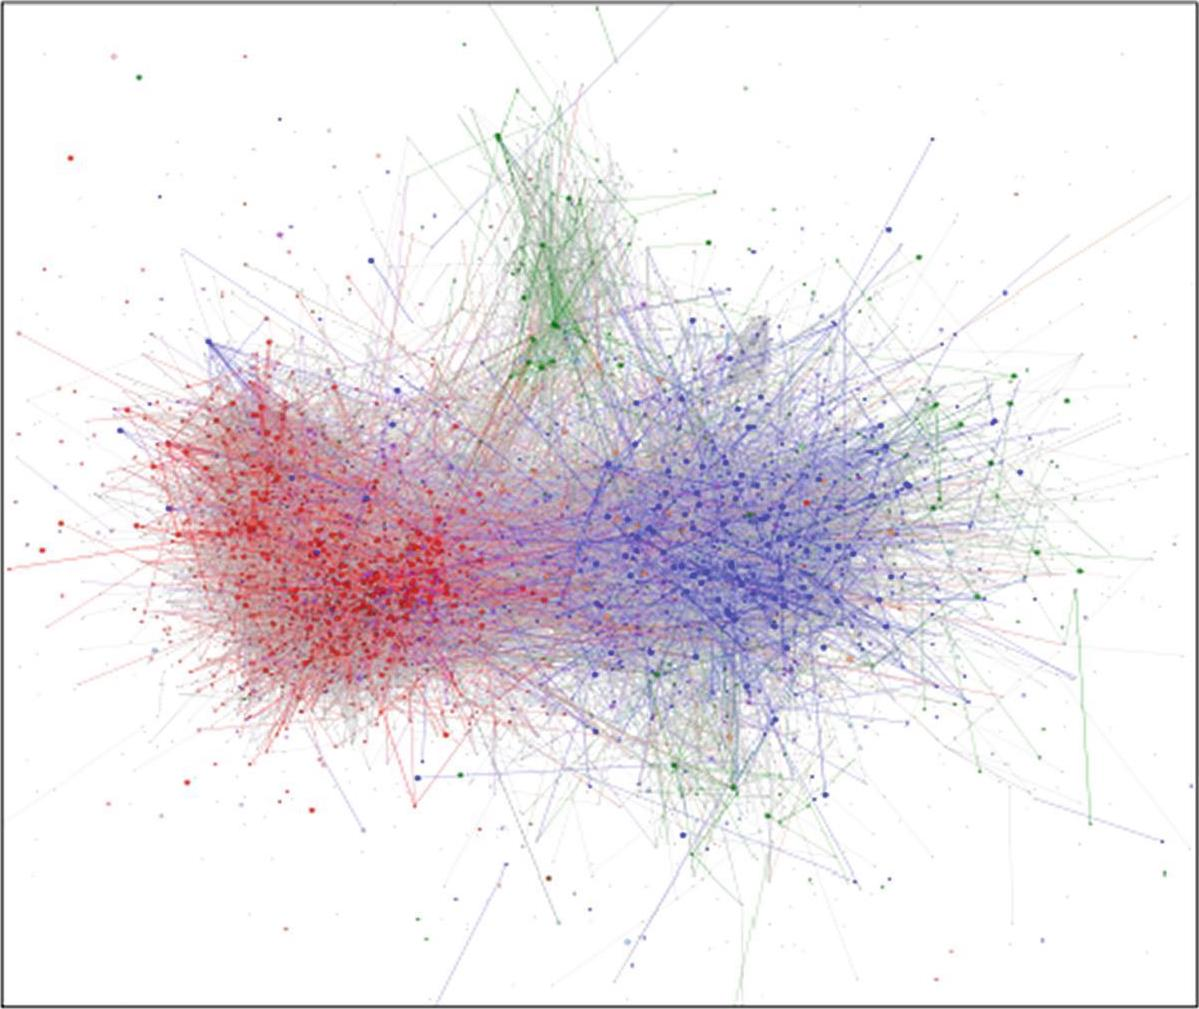
\includegraphics[width=0.419\linewidth]{yifanHuGraphs1}}
		\subcaptionbox{\label{fig:yifanHuGraphs-2}}{%
			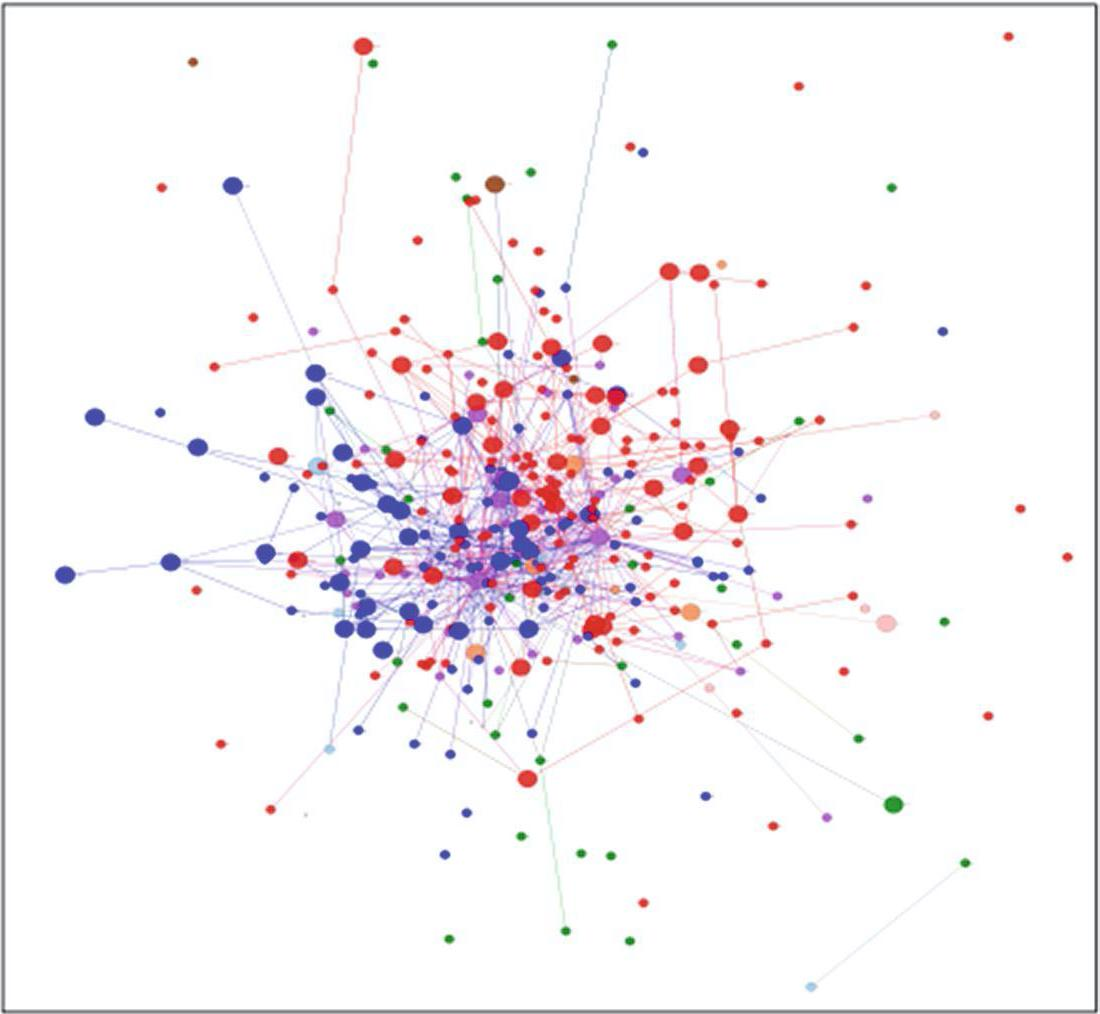
\includegraphics[width=0.382\linewidth]{yifanHuGraphs2}}
		\hfill
	}
	\caption{The YifanHu graphs (fragments) for language distribution in \cref{fig:yifanHuGraphs-1} \#jesuischarlie and \cref{fig:yifanHuGraphs-2} \#jenesuispascharlie. Red: French; blue: English; lilac: French/English; green: other European. (Color figure online)}\label{fig:yifanHuGraphs-12}
\end{figure}

Thus, H1a is proven; H1b is proven too but not due to ‘civilizational clashes’.

\textit{H2a/H2b.} To see the user grouping and sentiment cleavages within the French-speaking parts of the discussions, we have reconstructed the web graphs for them (see Fig.~\cref{fig:yifanHuGraphs-3} for \#jesuischarlie and Fig.~\cref{fig:yifanHuGraphs-4} for \#jenesuispascharlie, respectively).

\begin{figure}[ht]
	\centerfloat{
		\hfill
		\subcaptionbox[List-of-Figures entry]{\label{fig:yifanHuGraphs-3}}{%
			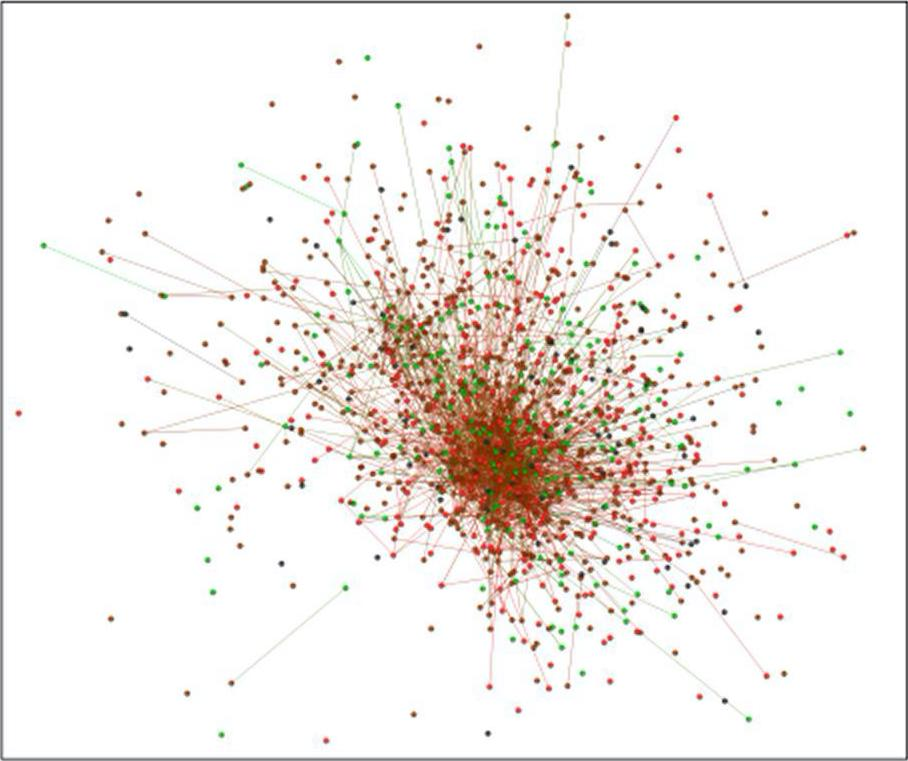
\includegraphics[width=0.419\linewidth]{yifanHuGraphs3}}
		\subcaptionbox{\label{fig:yifanHuGraphs-4}}{%
			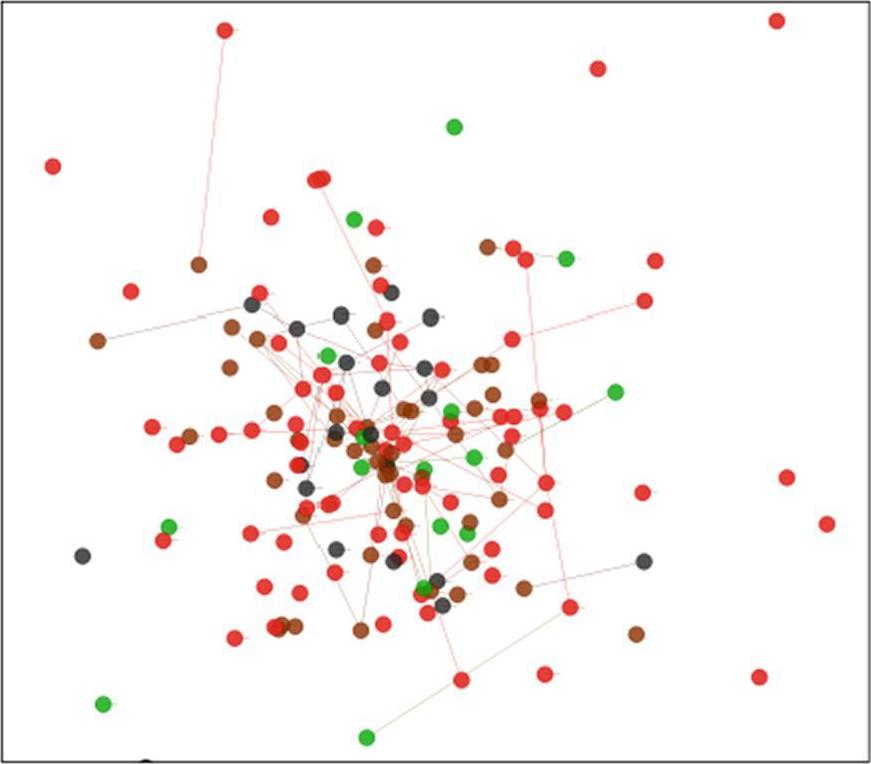
\includegraphics[width=0.4\linewidth]{yifanHuGraphs4}}
		\hfill
	}
	\caption{The YifanHu graphs (fragments) for language distribution in \cref{fig:yifanHuGraphs-3} \#jesuischarlie and \cref{fig:yifanHuGraphs-4} \#jenesuispascharlie. Red: French; blue: English; lilac: French/English; green: other European. (Color figure online)}\label{fig:yifanHuGraphs-34}
\end{figure}

Here, H2a should be rejected for \#jesuischarlie and partly supported for the second hashtag. Both in the graph and in the edge percentage calculations, it is only users with mixed sentiment who form a group (38.33\% against 56.05\% for the inter-group connections) in \#jesuischarlie. But for \#jenesuispascharlie, both mixed and negative user groups seem to have a potential for grouping (19.5\% and 15\% against 62.1\% for inter-group connections). Thus, H2b is supported: the cases do differ.

Even with the cases of such different sizes, H3 is supported: thanks to the negative nebula in \#jenesuispascharlie, we can state that echo chambers are able to form on at least two levels of the trans-border conflictual discussions of global (or, more precisely, macro-regional) reach. This adds to our understanding of the nature of public discussions in social media, even if lowers hopes for all-encompassing public spheres.

\subsection{Power laws in \textit{Ad Hoc} conflictual discussions on twitter. Digital Transformation and Global Society}\label{subsec:ch5/sec1/sub5}

\subsubsection{1. Introduction}

Public discussions online, and, of these, the ones on social networking sites, have become a growing area of scholarly attention, as they have been perceived as a manifestation of the public sphere, a crucial condition for efficient democratic deliberation \cite{Habermas}. Thus, understanding how networked discussions form and evolve is necessary for elaboration of proper criteria for their efficiency evaluation.

One of the issues recently raised by social science and communication scholars is that of comparability of the online discussions formed by the so-called issue publics \cite{Dahlgren}\cite[p.~422]{Habermas}. Such discussions form quickly (or even burst out) around events or burning issues. Due to their \textit{ad hoc} nature \cite{BrunsBurgess}, they may dissolve just as quickly, involve various actors, and are affective \cite{Papacharissi} and, thus, are shaped by emotions rather than by rational argumentation. The question remains whether we have grounds for comparing such discussions, as the differences in discussion substance may lead to critical differences in the discussion structure and connectivity, which would make, e.g., cross-cultural and cross-language comparisons of same-topic discussions impossible. Also, conclusions made for one discussion in terms of actor roles, dynamics, other constitutive parameters would not allow for predicting them for other discussions if the network structures are not assessed and recognized as similar.

This question has not yet been properly addressed in the social network analysis literature, as structural similarities of networked discussions, despite all the attention given to them, remain understudied in comparative perspective, especially in the view of the public sphere theory. The latter has elaborated its own vision of how to assess the efficacy of public discussions. Linking the two research areas for elaborating the SNA parameters for such assessment of the discussion networks would address one of the existing gaps in social network studies. For example, a number of more recent works have juxtaposed calculated and \textit{ad hoc} publics \cite{BrunsBurgess2015,LynnRosatiNair} in search of networking patterns of both types of discussions, but these studies were single-case, and we still lack the knowledge whether structural patterns vary across cases, cultures, and types of vocabularies used for data collection.

Another input for social network analysis from the public sphere theory would be addressing the difference between users who are key for the discussion outburst and random discussion participants. Traditional view would imply various manifestations of power distance between the two user groups, and one needs to know whether online discussions show stable patterns of differences between key and random users.

We address these research gaps by collecting data and analyzing web graph structures for five discussion outbursts about inter-ethnic (inter-national and inter-race) conflicts in the USA, Germany, France, and Russia of the 2010 s, reviewing altogether six discussion cases, as we split one into neutral and affective parts. We collect data from Twitter based on single hashtags and keyword conglomerates and show that there are repeatable structural patterns of the discussions across these cases.

The remainder of the paper is organized as follows. Section 2 discusses today’s literature on various aspects of discussion structure for comparative tasks. In Sect. 3, we describe the cases and formulate the hypotheses for their comparison. Section 4 shows and discusses the discovered results. In conclusion, we discuss applicability of our findings for further studies of online conflictual discussions.

\subsubsection{2. Comparing Discussion Structure on Social Networks: A Literature Review}

Ad hoc \textit{discussions: a plea for grounds for comparison}. Public discussions on social networking sites have drawn scholarly attention to their various aspects, including the connection between the deliberative power of ‘ordinary citizens’ and the platform and network features that might either empower or disempower user groups in their opinion expression, shape the discussion outcomes, and impact the respective decision-making, as well as inspire political mobilization via the ‘logic of connective action’ \cite{BennettSegerberg}. Thus, the discussions in online networks have been thoroughly studied in their substantial aspects. But one of the key issues in this research area is the principal possibility of comparisons between discussions on similar topics happening in various parts of the world and in varying times.

So far, comparative studies of cross-country social network discussions have been rare \cite{BodrunovaLitvinenkoBlekanov2017}; one of the reasons for that is the scholarly argument of low (or, rather, unknown) comparability of the discussions that are formed by the issue publics. This type of the discussion raises, arguably, the biggest amount of doubt ‘whether Habermas is on Twitter’ \cite{BrunsHighfeld2016}, as, from case to case, current research demonstrates varying results on echo chamber formation \cite{BastosMerceaBaronchelli,ColleoniRozzaArvidsson,Sunstein2001,YardiBoyd}, cross-group discussion potential \cite{Barbera,BarberaJostNagler}, and the roles of influencers detected by various means \cite{BastosRaimundoTravitzki,BodrunovaLitvinenkoBlekanov2017,DuboisGaffney}.

The reason for low comparability, as scholars argue, lies in the very nature of the discussions, as they are all \textit{ad hoc} -- that is, case-specific and random in formation. Such discussions have the outburst nature, may have varying patterns of dissolution, involve case-specific actors, and based on affect \cite{Papacharissi} -- that is, are shaped by emotions rather than by rational argumentation, which may add to the non-comparability of the discussions. Thus, the major research question is -- are \textit{ad hoc} discussions comparable in topical and sociological terms also comparable in the discussion structures? Or, in other words, are there structural features characteristic of such discussions, that would, ideally, distinguish them from other discussion types on social networks and on the Web on the whole? And what could be the markers for such \textit{ad hoc} discussion outbursts?

Today, in Twitter studies, there is scarce but growing evidence that \textit{ad hoc} discussions differ in their nature from other discussion types. Thus, several papers underline the differences between calculated and \textit{ad hoc} publics \cite{BrunsBurgess2015,LynnRosatiNair}, but no network parameters were used to prove the differences between these discussion types. Also, these studies were based on single cases, and we still lack the knowledge whether structural patterns for \textit{ad hoc} discussions vary or repeat across cases, cultures, and types of vocabularies used for data collection. This creates a focus for our enquiry.

\paragraph{Degree centralities as a proxy for discussion comparability and a potential discussion quality metric.} Degree centralities (in-degree, out-degree, and degree accumulating both of these) have been long ago recognized as the key structural metrics of user relations and random graph assessment \cite{AlbertBarabasi,BoccalettiLatoraMoreno,MisloveMarconGummadi}; degree distributions are recognized as a key variable describing users’ interest toward each other \cite{EdigerJiangRiedy}. At the same time, from the normative viewpoint relevant in social sciences, degree centralities are an important metric of user in-network influence \cite{BodrunovaLitvinenkoBlekanov2016}, as well as the metric important in deliberative terms: the more users are reached by the same user (or reach a given user, which is the same for non-directed graphs but not for directed graphs), the more probable is the chance for cross-opinion discussion. More importantly, it can also characterize general user involvement into the discussion in comparison with other discussions; in terms of user involvement, degree centralities are, arguably, the most telling. A range of more topic-specific research papers have also argued that degree-based metrics are useful for network-based studies of social conflict and dangerous networks. Of those, one work \cite{KarthinkaGeethaBose} has shown the importance of relational measures (as the authors noted, ‘who is related to whom’) in detecting the key attackers in the terrorist network.

There are, of course, several criticisms about degree distributions, as they gener- alize the network structure without taking into account the role of influencers (for the reviews on detecting and comparing influencer structures, see \cite{BodrunovaBlekanovMaksimov,BodrunovaLitvinenkoBlekanov2017,BodrunovaLitvinenkoBlekanov2016}), or ‘hub users’. Their roles, in various works, are assessed in different, if not directly opposite, ways. Thus, one stream of works insists on their disproportionately big role in information distribution (see \cite{BastosRaimundoTravitzki,DuboisGaffney}, and many others), while another line shows that such hubs may be inefficient due to their overload and incapability of transmitting information due to that \cite{HarriganAchananuparpLim}. But our goal is to test whether the discussions on the whole may be distinguished from Twitter on the whole.

As major research works in the area note \cite{BarabasiAlbert,BroderKumarMaghoul,HubermanAdamic}, due to preferential connectivity in real-world networks, a certain power law (just as its absence) in degree distribution may become the characteristic that describes specific network structures. Thus, networks expressing power-law-like degree distributions are known as scale-free \cite{AlbertBarabasi,EdigerJiangRiedy}, and ‘scale-free tweet mention graphs would imply that a few Twitter users and ‘mentioners’ are responsible for a disproportionately high fraction of a community’s discourse’ \cite[p.~587]{EdigerJiangRiedy}. Thus, degree distribution may serve as a proxy for, e.g., core vs. periphery assessment in terms of aggregate influencer power: it can tell whether the network is dominated by a small number of users \cite{YeWu}. Thus, for Twitter, it would allow for: (1) differentiating one network type from another; (2) proving that the discussions are similar in their core vs. periphery relations, which suits our research goals. Moreover, our previous studies \cite{BlekanovSergeevMaksimov2017} have shown that power law exponents, indeed, vary for different types of web structures; e.g. for university websites, the average exponent is 1.8 instead of the expected 2.1.

Early works on World Wide Web topology mentioned above, as well as other research papers (see, e.g., \cite{FaloustosFaloustosFaloustos}), all stated that power law distributions are characteristic for the Web on the whole. But another, later line of research papers has argued that the Web, by just evolving in time, has blurred the initial power-law-like degree distribution \cite{ChenChangGovindan,MeuselVignaLehmberg}. Smaller-scale research, though, tells that degree distributions are still valid for smaller real-world samples.

Today, more and more criticism is raised about the explanatory potential and the very existence of scale-free networks -- that is, of the power law in degree distributions -- in large human-based datasets \cite{BroidoClauset}. We, thus, want to test whether the certain power laws show up in ad hoc discussions, as distinguished from Twitter on the whole, cultivated long-term discussions, and random talk.

\paragraph{Power laws on Twitter: lack of comparative studies on the nature of the discussions.} So far, degree distributions have been studied for either the whole Twittersphere or its geographical segments; and, in these studies, the evidence on whether all the discussions on Twitter manifest power-law degree distributions is mixed.

Thus, cumulative degree distributions \cite{Newman} for Twitter on the whole studied a decade ago \cite{JavaSongFinin} showed that the slopes cin and cout [were] both approximately \(-2.4\). The authors have interpreted these figures as similar to those for the Web of those times (\(-2.1\) for in-degree, cf. \cite{DonatoLauraLeonardi}) and blogosphere (\(-2,38\), as based on Blogpulse conference dataset of 2003). With the latter claim, one could agree, but with the former one we would not, as our research shows that differences of 0.3 in exponent values may be characteristic of graph origin and/or discussion type \cite{BlekanovSergeevMaksimov2017}. Another study \cite{WengLimJiang} based on the data dated mostly from April 2008 to April 2009 and featuring the most followed Twitter users from Singapore has also demonstrated power-law-like degree distributions of the user networks. A Twitter-large study \cite{WelchSchonfeldHe} has shown a very different exponent value of \(-1.6\). But authors \cite{KwakLeePark} have crawled the whole Twittersphere and have not discovered any power law in link distribution on the global level, as other authors underline \cite{HansenArvidssonNielsen}.

Several studies have focused on country-based segments of Twitter. Thus, one study \cite{MyersSharmaGupta} has dealt with the Twitter follow graphs. The researchers have shown that in-degree and degree on Twitter are best fit by power law, while out-degree is best fit by log-normal distribution. Besides analyzing the entire Twitter, it also did country- based segment studies for Brazil, Japan, and the United States; very little variance was found between the countries in terms of in-degree, out-degree, and degree distribution \cite[p.~494]{MyersSharmaGupta}. Another study has dealt with the follow graphs of 10 country-bound Twitter segments around the world \cite{PobleteGarciaMendoza}. It has also demonstrated power-law in-degree and out-degree distributions, with power law coefficient ranging 5.91 to 9.51 and 8.12 to 13.62, respectively. But one also needs to note that user influencer status is linked much more to the number and activity levels of active followers (who retweet and/or mention a given user) than to the number of followers \cite{ChaHaddadiBenevenuto}; thus, one needs to look at the actual discussion graphs rather than at the graphs of following (much less linked to the real-world issue-based discussions) to more precisely determine the influential users, as well as to define the discussion type.

Even a fewer number of works have examined the degree distributions in hash- tagged discussions. We can name one work \cite{ZhouBandariKong} on Iranian elections; the discussion there also showed power law distributions, with in-degree being \(-2.85\) and out-degree being \(-2.42\), while the retweet-based network had in-degree of \(-1.94\). Another group of authors \cite{ConoverRatkiewiczFrancisco} have also observed that retweet- and mention-based networks virtually did not differ in their scale-free topology.

From the review above, one can conclude that scholarly evidence for power laws in degree distributions is greater than that of the opposite. But, despite their potential, degree distributions have not been tested for \textit{ad hoc} discussion outbursts in comparative perspective.

Our idea is to look how degree distributions work if we step-by-step eliminate the users with low degree index, starting from isolate users \((D = 0\)), and look at the cumulative degree distributions for each case.

\subsubsection{3. The Research Methodology}

\paragraph{The research questions.} Most of the available research proves that power laws are characteristic for Twitter ‘calm’ discussions, be it the whole Twitter or its parts, either hashtag-based or limited by region. But the exponent values of degree distribution vary highly, not allowing for any particular expectation. Thus, we ask: Will degree distribution of all the \textit{ad hoc} discussion be fit by a power law? Will the exponent values be similar, thus indicating that the discussions are similar? Will the exponent values differ from \(\lvert2.1\rvert\)? Will the exponent values be similar enough across world regions, hashtag- only / keyword conglomerates, and neutral / affective hashtags?

The research hypotheses that emerge of these research questions look as follows:

\begin{itemize}
	\item H1. All the discussions under scrutiny will be characterized by power law in degree distribution.
	
	\item H2. All the discussions will diverge from the \(\lvert2.1\rvert\) exponent value to the same direction and on comparable percentage. This includes hashtag vs. keyword conglomerates (H3).
	
	\item H4. Neutral and affective (expressing emotions of either sympathy and compassion or negation and hatred) hashtags will be comparable in their power law exponents.
\end{itemize}

\paragraph{The cases under scrutiny and their substantial comparability.} The cases of our attention all have the same set of features that is to ensure that the cases are comparable in sociological terms. Thus, all the cases have a violent trigger (a killing or rape/harassment) of inter-ethnic nature; the discussions are outburst -- that is, the number of users involved has one sharp peak and then slows down gradually; media report the communities to split into the minority, pro-minority majority, and anti-minority majority groups; there is peaceful protest or mass commemoration of the victims in the aftermath of the conflict; there is direct involvement of authorities of several levels into conflict resolution; and all the conflicts provoke a discussion on Twitter that gets to national (sometimes also to global) Twitter trending topics.

We are looking at the following cases (in chronological order):
\begin{itemize}
	\item A killing of a Russian Muscovite by an Uzbek immigrant and the subsequent anti- immigrant clashes in the Moscow district of Biryuliovo, Russia (2013);
	\item A killing of an African American teenager by a white police officer and the sub- sequent city riots in Ferguson, the USA (2014);
	\item The attack to the editorial office of Charlie Hebdo and the subsequent peaceful demonstrations in Paris, France (2015);
	\item The mass harassment of German females by male re-settlers from Middle East and North Africa in the New Year Eve in Cologne, Germany (2015--2016), and the subsequent protest meetings by PEGIDA and the ‘Alternative for Germany’ party;
	\item A bus attack at one of the Christmas markets in Berlin (2016).
\end{itemize}

In each case, the discussion data were collected and the respective web graph reconstructed; in the case of \textit{Charlie Hebdo}, two graphs (one for a neutral hashtag and one for a compassion hashtag) were reconstructed.

\paragraph{Data collection.} To collect the discussion bulk, we have created a specialized web crawler with adjustable modules \cite{BlekanovSergeevMartynenko}. It was done especially to overcome the well-known Twitter API limitations, like the ones on the number of requests to server and on the number of tweets available for download. It also bypasses the popularity algorithm and allows for human-like backfolding.

For bigger-scale discussions (Ferguson and Charlie Hebdo), one hashtag per graph was used. For smaller-scale discussions, snowballing reading of 1.000+ random tweets containing the primary hashtag/keyword was performed, thus bringing on keyword collections.

\begin{table} [htbp]%
	\centering
	\caption{The datasets collected.}%
	\label{tab:collectedDatasets}% label всегда желательно идти после caption
	\renewcommand{\arraystretch}{1.5}%% Увеличение расстояния между рядами, для улучшения восприятия.
	\begin{SingleSpace}
		\begin{tabulary}{\textwidth}{@{}>{\zz}L >{\zz}C >{\zz}C@{}} %Вертикальные полосы не используются принципиально, как и лишние горизонтальные (допускается по ГОСТ 2.105 пункт 4.4.5) % @{} позволяет прижиматься к краям
			\toprule     %%% верхняя линейка
			The case & The number of nodes & The number of edges \\
			\midrule %%% тонкий разделитель. Отделяет названия столбцов. Обязателен по ГОСТ 2.105 пункт 4.4.5
			Biryuliovo, 2013 & 11429 & 20106 \\
			Ferguson, 2014 & 169677 & 334050 \\
			\textit{Charlie Hebdo}, 2015 (neutral) & 952615 & 1782863 \\
			\textit{Charlie Hebdo}, 2015 (affective) & 719503 & 981131 \\
			Cologne, 2015--2016 & 40117 & 98508 \\
			Berlin, 2016 & 194937 & 298562 \\
			\bottomrule %%% нижняя линейка
		\end{tabulary}%
	\end{SingleSpace}
\end{table}

The initial datasets collected are represented in Table~\cref{tab:collectedDatasets}. Altogether, tweets by over 2 mln users were included into the research. Edges between the users were formed if any type of substantial interaction emerged between them (we counted retweets, mentions, and comments as such).

\paragraph{Web graph reconstruction and analytics.} We have reconstructed the graphs for each case. The graphs were non-directed, as we were interested in the aforementioned deliberative aspects of the discussions. We have used the OpenOrd algorithm for the graph reconstruction. This methods is based on calculating the maximum distance (in \%) between the two nodes and on a particular number of iterations (in all our cases, the algorithm converged the proposed 800 iterations to 750). This algorithm was chosen, as it brings to the discussion core (that is, to the center of the graph) the influential users defined by a wide set of variables, including absolute-figure ones (the number of tweets, likes, retweets, mentions, and comments) and centrality metrics (including degree, betweenness, parerank, and eigenvector centralities).

Then, the degree distribution exponents were calculated for each case, using eleven steps of isolate user elimination (for users with \(D = 0\) to 10 in the initial graph).

The results and answers to our hypotheses are presented below.

\subsubsection{4. The Research Methodology}

As stated above, we have calculated degree distribution exponents for each case. In order to clearly highlight the differences with the expected exponent value of \(\lvert2.1\rvert\) based on previous Web studies, we have also calculated the exponents for the eliminated users. The exponent values for both active users and eliminated users, as well as their absolute deviations from \(\lvert2.1\rvert\), are presented in Table 2. The degree distribution graphs are presented in Figs.~\cref{fig:biryuliovoDegreeDistribution},~\cref{fig:fergusonDegreeDistribution},~\cref{fig:charlieNDegreeDistribution},~\cref{fig:charlieADegreeDistribution},~\cref{fig:cologneDegreeDistribution} and~\cref{fig:berlinDegreeDistribution} for the respective cases, as ordered in Table~\cref{tab:caseExponentValues}.

\begin{table} [htbp]%
	\centering
	\caption{Exponent values for the cases and their divergence from the expects exponent value.}%
	\label{tab:caseExponentValues}% label всегда желательно идти после caption
	\renewcommand{\arraystretch}{1.5}%% Увеличение расстояния между рядами, для улучшения восприятия.
	\begin{SingleSpace}
		\begin{tabulary}{\textwidth}{@{}>{\zz}L >{\zz}C >{\zz}C >{\zz}C >{\zz}C@{}} %Вертикальные полосы не используются принципиально, как и лишние горизонтальные (допускается по ГОСТ 2.105 пункт 4.4.5) % @{} позволяет прижиматься к краям
			\toprule     %%% верхняя линейка
			The case & Exponent value, active users &  Absolute deviation, active users & Exponent value, eliminated users & Absolute deviation, eliminated users \\
			\midrule %%% тонкий разделитель. Отделяет названия столбцов. Обязателен по ГОСТ 2.105 пункт 4.4.5
			Biryuliovo, 2013 &  \(\lvert1.56\rvert \) & 0.54 & \(\lvert2.04\rvert\) & 0.06 \\
			Ferguson, 2014 & \(\lvert1.39\rvert\) & 0.71 & \(\lvert2.16\rvert\) &\( -0.06\)      \\
			\textit{Charlie Hebdo}, 2015 (neutral) & \(\lvert 1.59 \rvert\) & 0.51 & \(\lvert2.01\rvert\) & 0.09 \\
			\textit{Charlie Hebdo}, 2015 (affective) & \(\lvert1.80\rvert\) & 0.3 & \(\lvert2.45\rvert\) & \(-0.35\) \\
			Cologne, 2015--2016 & \(\lvert1.28\rvert\) & 0.82 & \(\lvert1.91\rvert\) & 0.19 \\
			Berlin, 2016 & \(\lvert1.63\rvert\) & 0.47 & \(\lvert2.34\rvert\) &  \(-0.24\) \\
			\bottomrule %%% нижняя линейка
		\end{tabulary}%
	\end{SingleSpace}
\end{table}

\begin{figure}[ht]
	\centerfloat{
		\hfill
		\subcaptionbox[List-of-Figures entry]{\label{fig:biryuliovoDegreeDistribution-1}}{%
			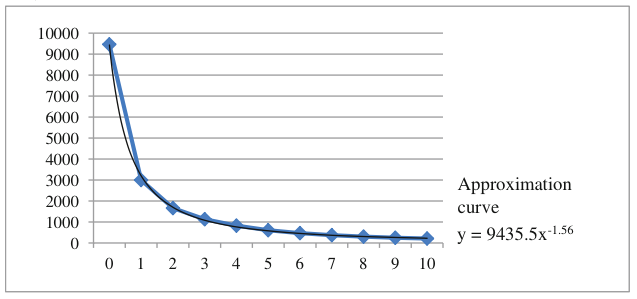
\includegraphics[width=0.5\linewidth]{biryuliovoDegreeDistribution1}}
		\subcaptionbox{\label{fig:biryuliovoDegreeDistribution-2}}{%
			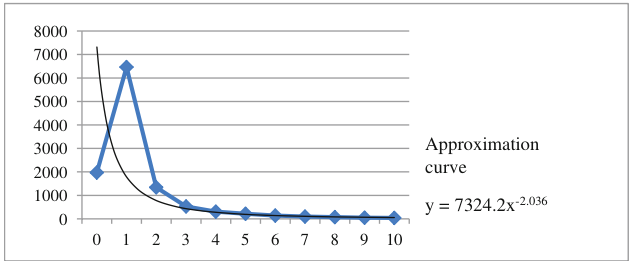
\includegraphics[width=0.56\linewidth]{biryuliovoDegreeDistribution2}}
		\hfill
	}
	\caption{Degree distributions for the Biryuliovo case: (а) active users; (б) eliminated users. \textit{Source:} authors.}\label{fig:biryuliovoDegreeDistribution}
\end{figure}

\begin{figure}[ht]
	\centerfloat{
		\hfill
		\subcaptionbox[List-of-Figures entry]{\label{fig:fergusonDegreeDistribution-1}}{%
			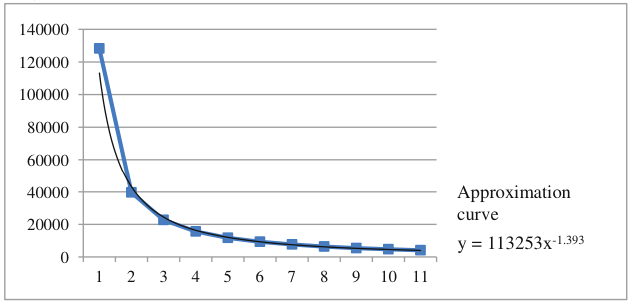
\includegraphics[width=0.509\linewidth]{fergusonDegreeDistribution1}}
		\subcaptionbox{\label{fig:fergusonDegreeDistribution-2}}{%
			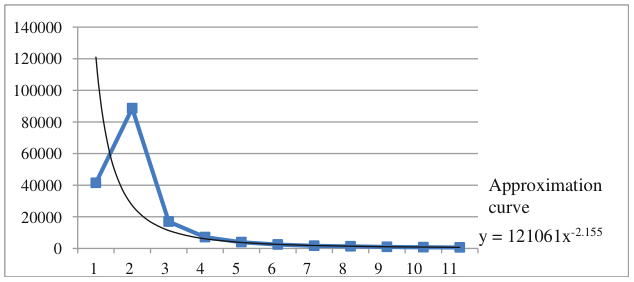
\includegraphics[width=0.55\linewidth]{fergusonDegreeDistribution2}}
		\hfill
	}
	\caption{Degree distributions for the Ferguson case: (а) active users; (б) eliminated users. \textit{Source:} authors.}\label{fig:fergusonDegreeDistribution}
\end{figure}

\begin{figure}[ht]
	\centerfloat{
		\hfill
		\subcaptionbox[List-of-Figures entry]{\label{fig:charlieNDegreeDistribution-1}}{%
			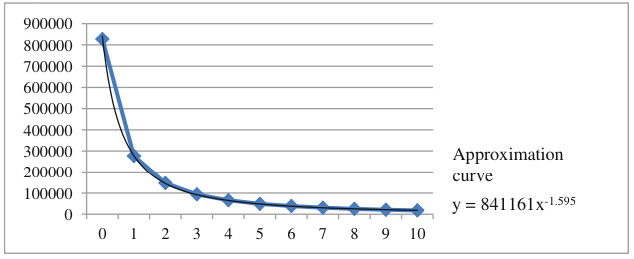
\includegraphics[width=0.56\linewidth]{charlieNDegreeDistribution1}}
		\subcaptionbox{\label{fig:charlieNDegreeDistribution-2}}{%
			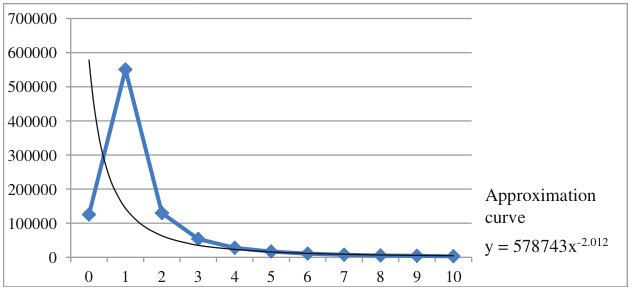
\includegraphics[width=0.5\linewidth]{charlieNDegreeDistribution2}}
		\hfill
	}
	\caption{Degree distributions for the \textit{Charlie Hebdo} neutral case: (а) active users; (б) eliminated users. \textit{Source:} authors.}\label{fig:charlieNDegreeDistribution}
\end{figure}

\begin{figure}[ht]
	\centerfloat{
		\hfill
		\subcaptionbox[List-of-Figures entry]{\label{fig:charlieADegreeDistribution-1}}{%
			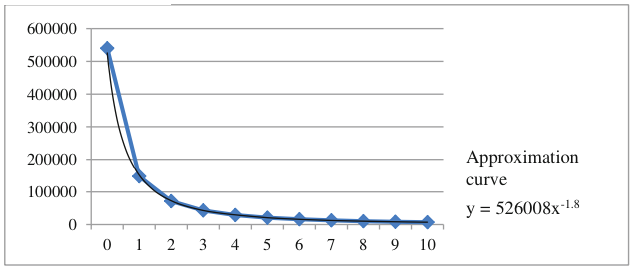
\includegraphics[width=0.5\linewidth]{charlieADegreeDistribution1}}
		\subcaptionbox{\label{fig:charlieADegreeDistribution-2}}{%
			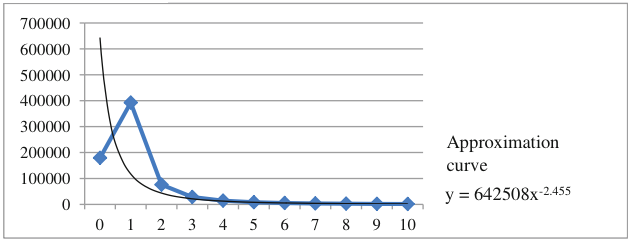
\includegraphics[width=0.55\linewidth]{charlieADegreeDistribution2}}
		\hfill
	}
	\caption{Degree distributions for the \textit{Charlie Hebdo} emotional case: (а) active users; (б) eliminated users. \textit{Source:} authors.}\label{fig:charlieADegreeDistribution}
\end{figure}

\begin{figure}[ht]
	\centerfloat{
		\hfill
		\subcaptionbox[List-of-Figures entry]{\label{fig:cologneDegreeDistribution-1}}{%
			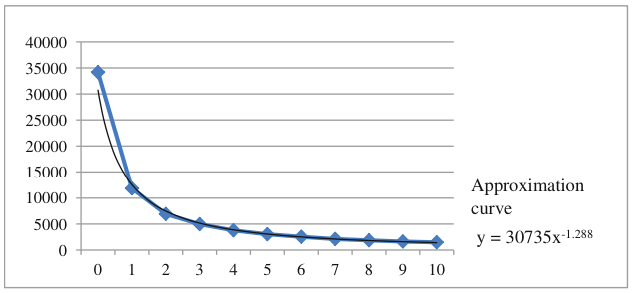
\includegraphics[width=0.51\linewidth]{cologneDegreeDistribution1}}
		\subcaptionbox{\label{fig:cologneDegreeDistribution-2}}{%
			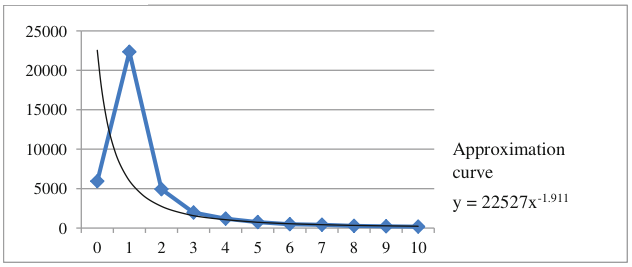
\includegraphics[width=0.55\linewidth]{cologneDegreeDistribution2}}
		\hfill
	}
	\caption{Degree distributions for the Cologne case: (а) active users; (б) eliminated users. \textit{Source:} authors.}\label{fig:cologneDegreeDistribution}
\end{figure}

\begin{figure}[ht]
	\centerfloat{
		\hfill
		\subcaptionbox[List-of-Figures entry]{\label{fig:berlinDegreeDistribution-1}}{%
			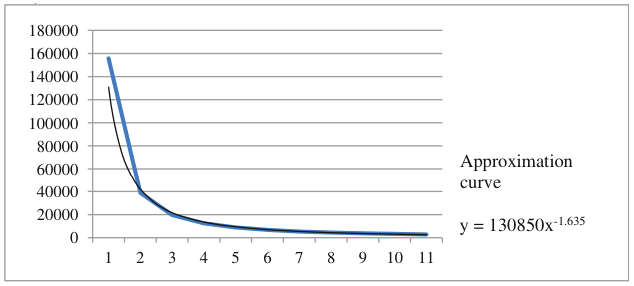
\includegraphics[width=0.51\linewidth]{berlinDegreeDistribution1}}
		\subcaptionbox{\label{fig:berlinDegreeDistribution-2}}{%
			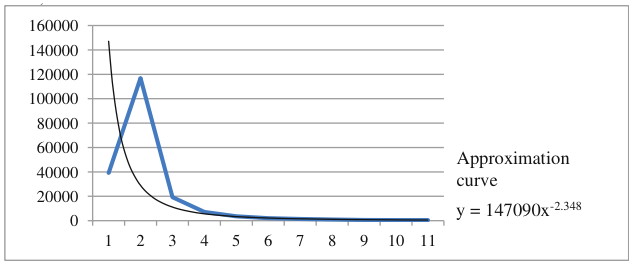
\includegraphics[width=0.55\linewidth]{berlinDegreeDistribution2}}
		\hfill
	}
	\caption{Degree distributions for the Berlin case: (а) active users; (б) eliminated users. \textit{Source:} authors.}\label{fig:berlinDegreeDistribution}
\end{figure}

\textit{H1.} All the cased that we have studied do, indeed, demonstrate power laws in degree distribution, and this is true for both active users (see Figs.~\cref{fig:biryuliovoDegreeDistribution-1},~\cref{fig:fergusonDegreeDistribution-1},~\cref{fig:charlieNDegreeDistribution-1},~\cref{fig:charlieADegreeDistribution-1},~\cref{fig:cologneDegreeDistribution-1} and~\cref{fig:berlinDegreeDistribution-1}) and eliminated users (see Figs.~\cref{fig:biryuliovoDegreeDistribution-2},~\cref{fig:fergusonDegreeDistribution-2},~\cref{fig:charlieNDegreeDistribution-2},~\cref{fig:charlieADegreeDistribution-2},~\cref{fig:cologneDegreeDistribution-2} and~\cref{fig:berlinDegreeDistribution-2}). Thus, power law is indicative for \textit{ad hoc} discussion outbursts across cultures and cases; H1 is supported.

\textit{H2.} All the cases do, indeed, diverge from the \(\lvert2.1\rvert\) expected exponent value to the same direction (see Table~\cref{tab:caseExponentValues}, column 2, exponent values for active users): the received exponent values are all equal or below 1.8, which indicates the lower power distance between the users. At the same time, the exponent values for eliminated users fluctuate around \(\lvert2.1\rvert\) to \(\lvert2.4\rvert\), the figures indicative for the Web degree distributions in various studies mentioned above. Thus, power laws with exponent values definitely below those discovered for the World Wide Web are indicative for \textit{ad hoc} discussions, which makes them, at least in terms of core vs. periphery relations, similar and comparable. The second part of the hypothesis is, though, not clearly supported: deviation from \(\lvert2.1\rvert\) substantially varies in percentage (from almost 40\% for the Cologne case to 14.3\% for \#jesuischarlie), and thus we cannot indicate any figure more precise than the fluctuation between \(\lvert1.28\rvert\) and \(\lvert1.80\rvert\) for ad hoc discussions; due to this, H2 is only partly proven. But we also need to state that, for three of six discussions, the exponent values were between \(\lvert1.56\rvert\) and \(\lvert1.63\rvert\), which corresponds to earlier results in \cite{WelchSchonfeldHe}.

\textit{H3.} For three of the six discussions (the Ferguson case and both Charlie Hebdo cases) the data were collected based on single hashtags (\#ferguson, \#charliehebdo, and \#jesuischarlie, respectively), while other cases were collected by keyword conglomerates ranging from 6 keywords (for the Biryuliovo case) to over a dozen keywords (for both German cases). As we see from Table~\cref{tab:caseExponentValues} and Figs.~\cref{fig:biryuliovoDegreeDistribution-1},~\cref{fig:fergusonDegreeDistribution-1},~\cref{fig:charlieNDegreeDistribution-1},~\cref{fig:charlieADegreeDistribution-1},~\cref{fig:cologneDegreeDistribution-1} and~\cref{fig:berlinDegreeDistribution-1}, there is no difference between single-hashtag and keyword-conglomerate data collection. H3 is supported, but this, paradoxically, might add not only to the evidence that \textit{ad hoc} discussions have similar patterns of degree distribution but also to the evidence that Twitter as a platform fosters the power law degree distributions in any type of discussion. To answer this, more research is needed.

\textit{H4.} As seen from Table~\cref{tab:caseExponentValues} and  Figs.~\cref{fig:biryuliovoDegreeDistribution-1},~\cref{fig:fergusonDegreeDistribution-1},~\cref{fig:charlieNDegreeDistribution-1},~\cref{fig:charlieADegreeDistribution-1},~\cref{fig:cologneDegreeDistribution-1} and~\cref{fig:berlinDegreeDistribution-1}, both neutral and affective hashtags are subjected to power law for both active and eliminated users, and exponent values deviate from \(\lvert2.1\rvert\) to the same direction. H4 is supported. We just need to mention that the compassion hashtag \#jesuischarlie has shown the highest exponent values, thus demonstrating bigger gaps between the influential and ‘peripheral’ users, and this might create room for further comparative investigations.

\paragraph{Discussion.} In search for proof of comparability of \textit{ad hoc} online discussions, we have applied our idea of evaluating degree distributions to six datasets of five comparable Twitter discussions on inter-ethnic conflicts in four countries that happened in the 2010 s. What we have discovered is the following.

First, we have shown that all the discussions we have observed are subjected to power law in degree distributions. Second, we have shown that exponent values for degree distributions in the discussion graphs diverge from the figures indicated for the Web on the whole in previous research. Moreover, they diverge in the same direction and to varying but, to a certain degree, also comparable percentage. Taken together, these findings indicate that, at least in terms of influence, interest, and/or power distribution in such discussions, they are comparable across countries and years, as well as across vocabulary types and neural/affective hashtags. Thus, exponent values may serve as indicators for the type of an online discussion. We have also shown that the peripheral part of the \textit{ad hoc} discussions was always closer to \(\lvert2.1\rvert\) to \(\lvert2.4\rvert\) exponent values discovered earlier for the Web and some social networks, which may be a sign that the \textit{ad hoc} discussions do differ from the ‘average’ network structure of the Web.

But we have also discovered that the exponent values for the discussions were fluctuating around \(\lvert1.6\rvert\) indicated earlier for Twitter on the whole; also, variance in value divergence from the expected figures was too big to state that a particular array of meanings may be indicative for ad hoc discussions and could become their structural marker. This needs further investigation, which might imply experimental design.

Last but not least, we have seen that \textit{ad hoc} discussions, if judged by the exponent values, show the patterns of lower power distance between core and periphery. This may be due exactly to their spontaneous nature, as institutional actors who shape and frame the offline discussions compete with ordinary users, crisis witnesses, and grassroots leaders. This may broaden our views upon discussion outbursts on social media.

\section{Тематическое моделирование контента}\label{sec:ch5/sect2}

\subsection{Topic modeling of conflict ad hoc discussions in social networks}\label{subsec:ch5/sec2/sub1}

\subsubsection{Introduction}

As a result of different media platforms achieving a steady user growth in a recent years more and more people begin to use different social networks as the main source of news on economical, political and social events. In particular, ad hoc discussions emerged which can be defined as a debate about a specific problem. In most cases such discussions appear in the case of controversial events and involve large number of participants.

Presence of such user activity raises the problem of analyzing large volumes of this type of data which has become one of the most important problems in many data analysis tasks, including topic modeling. Topic modeling algorithm in this case is an algorithm that, given the number of topics and the list of user messages can output two distributions: topics over documents and of words over topics. Such algorithm can help in the understanding of different points of view and highlight the main arguments. This can be useful in many ways one of which is the case in which the number of documents is big and we want to know their general content without reading them all. Another use case is data prepossessing, reducing the dimensions of data to use in other analysis tasks such semantic analysis. However directly applying traditional topic models like LDA and PLSA to short texts can be problematic primarily due to the sparsity of data given the specificity of short texts. In this paper we are studying the usage of different models on a large scale data which can effectively infer hidden topics in big discussions taking these features into account.

\subsubsection{Prior Work}

Early studies of the problem of topic modeling on short texts mainly concerned the use of external knowledge to improve the representation of text data. For example, Phan and others \cite{HoriguchiPhanNguyen} used the modeling of those short texts based on the traditional topic model, the effectiveness of which was tested on a large-scale data set for the purpose of short texts classification. In these works, it is assumed that the use of data derived from long texts could help improving the model for short texts. However, these methods are effective only when the auxiliary data are closely related to the original data. In the case of texts, obtained from social networks this task is impossible due to most of user messages being self-contained. Another assumption is based on the use of different aggregation methods. In the case of data, obtained from the Twitter, user messages can be aggregated by authors, publication time and hashtags. The \cite{WrayLexingRishabh} shows that the best performing method is based on hashtag based aggregation, however it can’t be applied then the texts themselves are collected using a series of hashtags (which is one of better ways for collecting data on big events). Author based aggregation can also be unreliable since the majority of users will have very few messages on any given topic. In this paper we are focusing on models, relying on statistical information about the data.

\subsubsection{Topic Models}

\paragraph{LDA.} Latent Dirichlet Allocation is a three-level hierarchical Bayesian model in which each element of the collection is modeled as a finite distribution over the set of topics. Each topic, in turn, is modeled as an infinite mixture by the set of topic probabilities \cite{MichaelJohnDavidAndrew}.

Lda assumes the following generative process:
\begin{itemize}
	\item Choose \(\theta_i \sim \textit{Dir}(\alpha)\)
	\item Choose \(\phi_i \sim \textit{Dir}(\beta)\)
	\item For every word position \(i, j\):
	\begin{itemize}
		\item Choose a topic \(z_{i, j} \sim \textit{Multinomial}(\theta_i)\)
		\item Choose a word \(w_{i, j} \sim \textit{Multinomial}({\phi_z}_{i,j})\)
	\end{itemize}
\end{itemize}
The model parameters \(\alpha\) and \(\beta\) are typically chosen sparse for better performance on short texts. In this paper, LDA is used as a baseline model, the effectiveness of which for standard texts has been proven both theoretically and in many experimental results.

\paragraph{BTM.} Biterm Topic Model performs topic modeling task by modeling a set of biterms (unordered word pair cooccurring in a short context). The main idea is that if two words co-occur more frequently, they are more likely to belong to a same topic \cite{YanyanJiafengXueqi}.

Btm assumes the following generative process:
\begin{itemize}
	\item Draw \(\theta_i \sim \textit{Dir}(\alpha)\)
	\item For each topic \(k\):
	\begin{itemize}
		\item draw \(\phi_k \sim \textit{Multinomial}(\beta)\)
	\end{itemize}
	\item For each biterm \(b_i\):
	\begin{itemize}
		\item draw \(z_i \sim \textit{Multinomial}(\theta)\)
		\item draw \(w_{i,1},w_{i,2} \sim \textit{Multinomial}({\phi_z}_i)\)
	\end{itemize}
\end{itemize}

As BTM does not model documents explicitly, we must provide a way to infer the topics in a document, i.e., evaluating the topic posterior. Using the chain rule the following equation was obtained:
\begin{equation}
	\label{eqn:29}
	P(z \mid b) = \sum P(z \mid b_i) P(b_i \mid d)
\end{equation}

Where \(P (z \mid b_i)\) can be obtained using via Bayes’ formula based on the parameters learned in BTM and \(P(b_i \mid d)\) can be calculated using empirical distribution of words in a document.

\paragraph{WNTM.} Word Network Topic Model’s idea is based on the following observations. When the texts are short, the word-document space is very sparse, but the word-word space still contains a large number of non-zero elements. Since the topic distribution for each doc- ument can not be recognized accurately in short or unbalanced texts, instead WNTM uses the topic distribution for each word \cite{KeYuanJichang}. Therefore, WNTM studies the distribution by topics for words, rather than those for documents. Studying the topics of the word, rather than those of the document make WNTM less sensitive to the length of the document. In addition, a network of words can be built with any type of text, which makes the WNTM model simple and universal in real applications, unlike other models, such as the mixture of unigrams \cite{ThrunMitchellNigam} and BTM.

The generative process of the model is in many respects similar to that of the LDA, but due to the use of a different distribution it has its own features:
\begin{itemize}
	\item For every latent word group \(z\) choose \(\phi \sim Dir(\beta)\)
	\item Choose \(\vartheta_i \sim \textit{Dir}(\alpha)\) distribution of a latent word group for adjacent word list \(L_i\) for word \(w_i\)
	\item For every word \(w_j \in L_i\):
	\begin{itemize}
		\item Choose a latent word group \(z_j \sim \vartheta_i\) 
		\item Choose an adjacent word \(w_j \sim {\phi_z}_j\)
	\end{itemize}
\end{itemize}

\begin{figure}[ht]
	\centerfloat{
		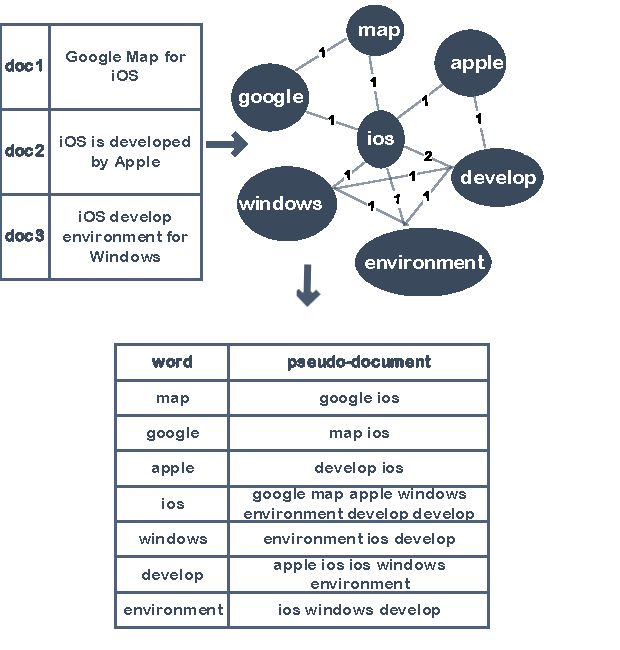
\includegraphics[scale=1.0]{wntmGeneration}
	}
	\caption{Generation of word network for WNTM model \cite{KeYuanJichang}.}\label{fig:wntmGeneration}
\end{figure}

Similarly to BTM this model can’t be directly applied to get topic distributions over documents. To get the topics in the document, we assume that the proportions of the words generated by the document is equal to the proportions of the document topics, that is:
\begin{equation}
	\label{eqn:30}
	P(z \mid d) = \sum P(z \mid w_i) P(w_i \mid d)
\end{equation}
Where \(P(z \mid w_i\)) equal \(\vartheta_{i,z}\), obtained in the generative process of WNTM and \(P(w_i \mid d)\) obtained as an empirical distribution of words in documents.

\subsubsection{Experiment}

The experiment was conducted to evaluate the quality of these three models, on three sets of ad hoc discussions. The following coherence measures were used to test the effectiveness of each model:

\begin{itemize}
	\item UMass \cite{MimnoWallachTalley} measures how often a common word of each topic is in average a good predictor for a less common word.
	\item NPMI \cite{StevesonAletras} is a normalized version of pointwise mutual information.
\end{itemize}

\paragraph{Data sets.} In this work models were tested on data, collected on three ad hoc discussions from Twitter social network: Riots in Biryulevo (Russia), October 2013 \cite{BodrunovaLitvinenkoBlekanov}, Ferguson unrest (USA), August 2014 \cite{SmoliarovaBlekanovBodrunova} Charlie Hebdo shooting (France), January 2015 \cite{SmoliarovaBlekanovLitvinenko}. The data was crawled based on hashtags in user messages.

\textit{Byrulevo. Riots in Biryulevo}
\begin{itemize}
	\item Total number of user messages: 10215
	\item Total number of users participated in the discussion: 11429
	\item Surveyed time period: 1.10.2013 - 31.10.2013
	\item Number of users who published tweets in the period under consideration: 3574
\end{itemize}

\textit{Ferguson. Ferguson unrest}
\begin{itemize}
	\item Total number of user messages: 193812
	\item Total number of users participated in the discussion: 169677
	\item Surveyed time period: 22.08.2014 - 31.08.2014
	\item Number of users who published tweets in the period under consideration: 70018
\end{itemize}

Charlie Hebdo. Charlie Hebdo shooting
\begin{itemize}
	\item Total number of user messages: 505069
	\item Total number of users participated in the discussion: 952615
	\item Surveyed time period: 07.01.2015 - 10.01.2015
	\item Number of users who published tweets in the period under consideration: 238491
\end{itemize}


\begin{table}[ht]%
	\centering
	\caption{Topics for Byrulevo data set.}%
	\label{tab:byrulevoTopics}% label всегда желательно идти после caption
	%	\begin{adjustbox}{width=1\textwidth}
		%		\small
		\begin{tabular}{ c  c  c  c }% Вертикальные полосы не используются принципиально, как и лишние горизонтальные (допускается по ГОСТ 2.105 пункт 4.4.5) % @{} позволяет прижиматься к краям
			\toprule
			Topic 1 & Topic 2 & Topic 3 & Topic 4 \\
			\hline
			\multicolumn{4}{c}{\makecell{LDA}} \\
			migrant & warehouse & broadcast & riot  \\
			Zeynalov & work & live & Manezhka \\
			police & man & moscow & moscow \\
			murder & boutique & photo & migrant \\
			Sherbakov & moscow & find & block \\
			\hline
			\multicolumn{4}{c}{\makecell{WNTM}} \\
			Moscow & news & Moscow & police \\
			event & Sherbakov & OMON & authorities \\
			Russia & migrant & Zeynalov & killer \\
			riot & murder & arrest & russian \\
			mayhem & killer & Sherbakov & meetings \\
			\hline
			\multicolumn{4}{c}{\makecell{BTM}} \\
			citizen & OMON & Sherbakov &  russian \\
			police & warehouse & Zeynalov & government \\
			local & police & killer & riot \\
			riot & arrest & arrest & migrant \\
			Moscow & killer & moscow & news \\
			\bottomrule
		\end{tabular}%
		%	\end{adjustbox}
\end{table}

\begin{table}[ht]%
	\centering
	\caption{Topics for Charlie Hebdo data set.}%
	\label{tab:charlieTopics}% label всегда желательно идти после caption
	%	\begin{adjustbox}{width=1\textwidth}
		%		\small
		\begin{tabular}{ c  c  c  c }% Вертикальные полосы не используются принципиально, как и лишние горизонтальные (допускается по ГОСТ 2.105 пункт 4.4.5) % @{} позволяет прижиматься к краям
			\toprule
			Topic 1 & Topic 2 & Topic 3 & Topic 4 \\
			\hline
			\multicolumn{4}{c}{\makecell{LDA}} \\
			policia & die & police & islam \\
			Paris & satire & shooting & religion \\
			terroristas & cartoonist & attack & youngest  \\
			sospechosos & frankreich & suspects & local \\
			ataque & attentater & update & extrimists \\
			\hline
			\multicolumn{4}{c}{\makecell{WNTM}} \\
			attack & suspects & cartoonists & media\\
			french & police & support & cartoons  \\
			today & two & editor & toxic \\
			terror & attack & respond & image \\
			killed & hostage & journalism & caricatures \\
			\hline
			\multicolumn{4}{c}{\makecell{BTM}} \\
			police & french & victims & muslims\\
			suspects & shooting & solidarity & islam \\
			hostage & gunman & attack & must \\
			killed & dead & France & say\\
			breaking & killed & jesuischarlie & religion \\
			\bottomrule
		\end{tabular}%
		%	\end{adjustbox}
\end{table}

\begin{table}[ht]%
	\centering
	\caption{Topics for Ferguson data set.}%
	\label{tab:fergusonTopics}% label всегда желательно идти после caption
	%	\begin{adjustbox}{width=1\textwidth}
		%		\small
		\begin{tabular}{ c  c  c  c }% Вертикальные полосы не используются принципиально, как и лишние горизонтальные (допускается по ГОСТ 2.105 пункт 4.4.5) % @{} позволяет прижиматься к краям
			\toprule
			Topic 1 & Topic 2 & Topic 3 & Topic 4 \\
			\hline
			\multicolumn{4}{c}{\makecell{LDA}} \\
			police & MikeBrown & militarization & Miami  \\
			life & black & police & overtown \\
			surrender & brown & law & America \\
			must & racism & reason & vote  \\
			dissa & justice & end & jail \\
			\hline
			\multicolumn{4}{c}{\makecell{WNTM}} \\
			MikeBrown & CNN & must & movement  \\
			amp & cops & surrender & speak \\
			police & Times & police & join  \\
			black & black & dissa & support \\
			people & shooting & see & now\\
			\hline
			\multicolumn{4}{c}{\makecell{BTM}} \\
			must & join & community & pd\\
			police & movement & Miami & look \\
			surrender & now & support & closer  \\
			dise & speak & lot & MikebBrown  \\
			click & die & overtown & msnbc \\
			\bottomrule
		\end{tabular}%
		%	\end{adjustbox}
\end{table}

\paragraph{Results.} Coherence measures were calculated and plotted to estimate the models’ effectiveness on different number of topics. The results (Figures~\cref{fig:charlieCoherence,fig:byrulevoCoherence,fig:fergusonCoherence}) allow us to talk about the approximate number of topics that is optimal for this task, but due to imperfection of quality indicators it requires manual clarification.

\begin{figure}[ht]
	\centerfloat{
		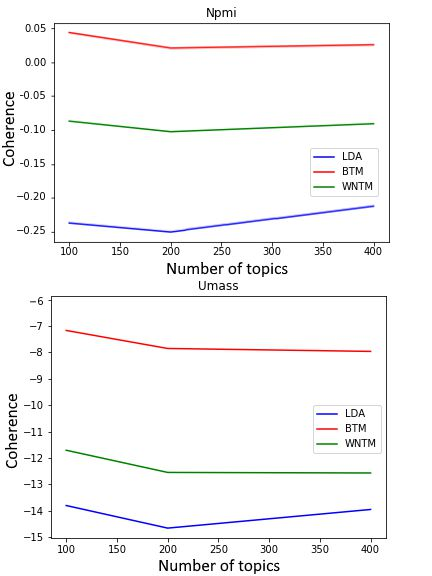
\includegraphics[scale=1.0]{charlieCoherence}
	}
	\caption{Coherence scores on Charlie Hebdo data set.}\label{fig:charlieCoherence}
\end{figure}

\begin{figure}[ht]
	\centerfloat{
		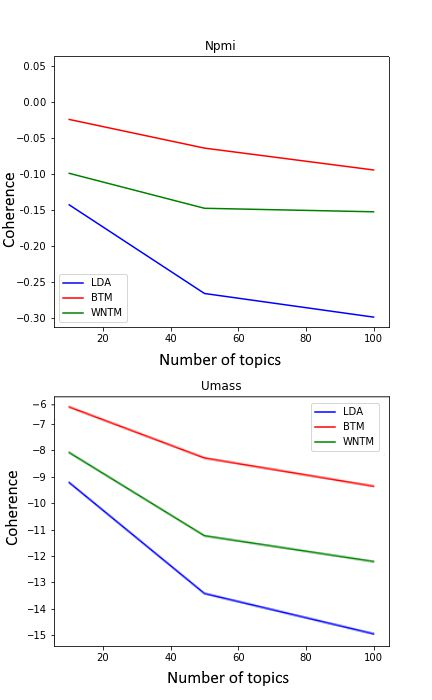
\includegraphics[scale=1.0]{byrulevoCoherence}
	}
	\caption{Coherence scores on Byrulevo data set.}\label{fig:byrulevoCoherence}
\end{figure}

\begin{figure}[ht]
	\centerfloat{
		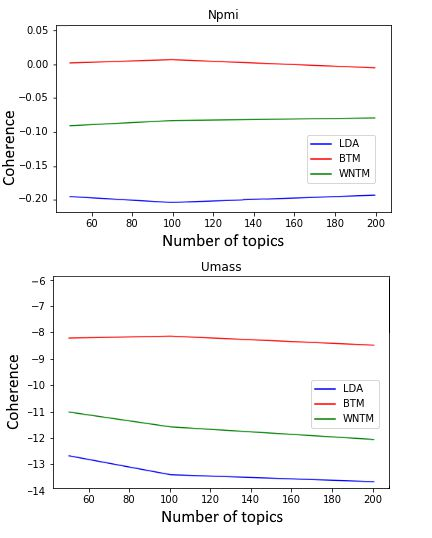
\includegraphics[scale=1.0]{fergusonCoherence}
	}
	\caption{Coherence scores on Ferguson data set.}\label{fig:fergusonCoherence}
\end{figure}

For each data set and topic model a few most coherent topics (topics focused on specific words which have the higher probability to occur in a specific topics) were chosen and can be seen in Tables~\cref{tab:byrulevoTopics,tab:charlieTopics,tab:fergusonTopics}.

As a result of the analysis of the given conflict ad hoc discussions, Biterm Topic Model came out to be the best performing and most stable method based on all coherence measures, baseline Lda model not specialized for working with short text has shown to not be suitable without the additional preprocessing of data mainly due to the data sparsity. However topics identified using this model can still be used to analyze key moments of discussions, participants’ arguments, and as a basis for other data analysis tasks.

Future work involves continuing the work on peer review, the first part of which was done for the Byrulevo data set by students and researchers from the journalism department of SPBU university. It has shown that the best results were obtained by the WNTM model. Comparing results of the models to the manual evaluation will allow us to measure not only the effectiveness of each model but also to compare coherence measures and find which one correlates better with human perception. The different prepocessing methods can also be used to improve the final result, tf-idf can be used instead of regular bag words approach to omit less frequent words more effectively.

\subsection{The ideal topic: interdependence of topic interpretability and other quality features in topic modelling for short texts}\label{subsec:ch5/sec2/sub3}

\subsubsection{1. Introduction}

The studies of large text corpora via automated detection of topicality are a growing area of social research. Topic modelling is a probabilistic tool for discovering non-evident topics in a collection of texts. After the potential of topic modelling for Twitter has been proven \cite{RamageDumaisLiebling}, it has become a separate and growing area within topic detection research. Several works have shown that topic modelling of Twitter data is suitable for both detection of hidden discussion topics and data pre-processing aimed at reducing the topical dimensionality of the studied corpora \cite{BlekanovTarasovMaksimov,KoltsovaKoltcov}, as well as for a range of comparative tasks. In both capacities, it has already been applied to practical tasks like drug use analysis \cite{JonnagaddalaJueDai} or assessment of popular behavior during natural disasters \cite{LigutomOrioRamacho,MacedaLlovidoPalaoag}.

But, despite the promise, topic modelling is highly problematic when applied to short texts \cite{MazaruraDeWaalKanifer}, especially of the oral-written nature \cite{Lutovinova} often met online, of which Twitter is exemplary. Short texts, including Twitter posts (tweets), are today a popular form of public speech online, but their nature creates substantial obstacles to modelling topicality in Twitter corpora of virtually any size.

Topic modelling algorithms for the English language on Twitter have been explored widely, even if not extensively. Several models beyond LDA with Gibbs sampling, such as vector models or pLSA, as well as extensions for LDA, have been proposed. In most cases, classic unsupervised LDA performed worse than extended LDA or other models like biterm topic modelling (BTM). But, in some cases, LDA is used unquestioned, with results interpretable enough; this is why we will compare LDA which is in wide use with two other models described below.

Till today, comparative works on Twitter topic models for various languages beyond English remain very rare, mostly focusing on German and Spanish. Comparative studies of topic modelling for the francophone segment of Twitter are truly scarce, and, for the Russian-language Twitter, except for the earlier pilot works by our working group \cite{RamageDumaisLiebling,BlekanovTarasovMaksimov,SmoliarovaBodrunovaYakunin}, are almost non-extant. For a rare comparative work on five languages including French and Russian. This work, similar to ours in its goals, tests three models of topic detection, including the authors’ own development, and tests them by human coders and objective measures. The paper reports the comparative results on topic coherence and the so-called ‘utility’ of topic clusters (not topics!) without explaining how utility relates to human interpretability (whether this actually is interpretability or not). The authors also claim that their own model performs better than both LDA and BTM, but they do not reveal its full details for that would allow for comparison of the algorithms. Moreover, the results are not presented in full but, e.g. for all the languages beyond English, only on LDA and the authors’ model. Due to these reasons, we will look to French and Russian to once again compare the quality of topic detection.

Another gap in the current research on Twitter topics detection is that, except for e-health and natural disasters, issue- or event-oriented discussions are practically not studied. The methodological papers, including \cite{Sridhar}, do a lot to avoid limitations to overall Twitter topicality and work with large data that contain all possible topics. But, within a case-oriented discussion, detection of topics must be seriously complicated by the fact that the inner sub-topics share very similar lexicons.

To partly cover these gaps, we have taken under scrutiny three conflictual cases in three different countries, as they have provoked the respective Twitter discussion of a large scale but at the same time were focused enough for our experiment. In our earlier research, we have applied unsupervised LDA, as well as WNTM and BTM, to these three cases (see below), with BTM showing the best results by automated quality assessment metrics, namely Umass and NPMI \cite{BlekanovTarasovMaksimov}. But here we need to re-discuss our conclusions and juxtapose them to other, more subjective quality metrics such as topic saliency and human interpretation. Also, we try to see whether topic saliency and topic interpretability are linked to each other; to our best knowledge, this idea has not yet been explored by the academic community.

The remainder of the paper is organized as follows. In Sect. 2, we discuss the topic modelling algorithms that we use and the results we have received by applying the automated quality metrics and human coding, with the conclusion to reject both baselines. In Sect. 3, we present our ideas on the two other measures of topic detection quality, namely topic saliency and topic robustness. Section 4 serves for describing the cases and formulating the hypotheses. Section 5 provides the description of methods. In Sect. 6, we present the results and discuss them. To conclude, we formulate our idea of the ‘ideal topic’.

\subsubsection{2. Human and Automated Evaluation of Quality: Rejection of Both Baselines}

\paragraph{2.1 Automated Quality Assessment}

For automated quality assessment, we have used the coherence metrics that have gained popularity in the recent academic research, namely Umass and normalized PMI (NPMI). As we have shown in our earlier pre-tests, by both metrics, we have seen BTM to be performing better than the two other algorithms \cite{BlekanovTarasovMaksimov}.

But, after preliminary evaluation by human coders, we have seen that there are problems in topic interpretation that are not captured by the topic coherence metrics. Thus, the problems that we have discovered may be summarized as follows: 1) seemingly low number of interpretable topics; 2) a relatively big number of topics too similar to each other; 3) one-retweet-based topics gathered around one popular tweet rather than around a real topic in the discussion; 4) chained topics that unite several micro-themes but are non-clear to the human coders.

\paragraph{2.2 Human Coding and Its Artifacts}

Interpretability is understood here as an ability of a human coder to say why the topic descriptors (the most relevant words that describe the topic) stay together in a given topic. This is a traditional and ultimate metric of topic quality, as human interpretability is the ultimate goal of the whole modelling procedure. But this metric is non-feasible if the number of topics in multiple runs of the algorithms is overwhelming.

Interpretability is really hard to measure in an objective way. Moreover, below we show that human coding is critically dependent on three types of knowledge: that on the case, that on method, and that on the dataset. The difference in preparation to coding critically alters the coding results.

In Table~\cref{tab:coderTrainingArtifacts}, we show the coding results for three pairs of coders: unexperienced coders who have no detailed knowledge on the case, unexperienced coders who have received detailed instructions on the case and a lot of background knowledge, and members of our working group who have knowledge on the case, the dataset, and the algorithms.

\begin{table}[ht]%
	\centering
	\caption{Human coding of the Russian dataset, 100 topics: the artifacts of coder training.}%
	\label{tab:coderTrainingArtifacts}% label всегда желательно идти после caption
	%	\begin{adjustbox}{width=1\textwidth}
		%		\small
		\begin{tabular}{ c  c  c  c  c  c  c }% Вертикальные полосы не используются принципиально, как и лишние горизонтальные (допускается по ГОСТ 2.105 пункт 4.4.5) % @{} позволяет прижиматься к краям
			\toprule
			 & \multicolumn{2}{c}{\makecell{Unexperienced}} & \multicolumn{2}{c}{\makecell{Trained}} & \multicolumn{2}{c}{\makecell{Experienced}}\\
			\cline{2-7}
			& Coder 1 & Coder 2 & Coder 1 & Coder 2 & Coder 1 & Coder 2\\
			\hline
			LDA & 33\% & 11\% & 65\% & 94\% & 53\% & 63\% \\
			WNTM & 12\% & 11\% & 75\% & 92\% & 76\% & 73\%\\
			BTM & 22\% & 8\% & 88\% & 86\% & 76\% & 83\%\\
			\bottomrule
		\end{tabular}%
		%	\end{adjustbox}
\end{table}

As we see from Table~\cref{tab:coderTrainingArtifacts}, the coding result is, indeed, highly skewed by the coder background knowledge. Also, experienced coders from the working group show the tendency to give out a more balanced coding output, as they are more strict on the method performance and do not imply the inner grammar relations to the topics, filtering interpretability by the knowledge on the internal discourses in the dataset.

Thus, we see both automated dataset-level and human-based topic-level metrics to be unreliable in terms of finding ‘real topics’. This is why we suggest two other metrics and test their interconnectedness with human interpretability, to be able in future to substitute human coding by measuring these metrics.

\subsubsection{3. Topic-Level Quality Assessment: In Search of Independence Form Human Eye}

Thus, we have decided to introduce topic-level metrics of quality of topic modelling and test whether human interpretability will be related to them; we do it in an attempt to find topic-level metrics to substitute human coding without the necessity to assess the quality of the algorithm. At the same time, we still consider the well-known \textit{tf-idf} metric relevant for topic quality detection and will test our metrics against it in future.

\paragraph{3.1 Topic Saliency}

The idea of topic saliency lies in the fact that, for various time slots within a discussion, different sub-themes may emerge as the leading ones. Saliency is calculated in the following way. Each document in the dataset is assigned a topic distribution; then, based on the time of publication, the topic distributions in the tweets are summarized, and, for each topic, the saliency is calculated as the sum of the tweets belonging (with a certain probability) to the particular topic. Since the intensity of the discussion may vary in time, the overall topic saliency for all topics may vary (from 0 to 1, in our case). We have used a 24-h step and measured the topic saliency for each day in aggregate. This strategy constitutes one of the limitations for our study, as the French dataset encompasses four days only, due to its overwhelming volume (see below); in future, for the 4-day French dataset, we plan to change the step and conduct an hourly analysis.

To our best knowledge, topic saliency has not yet been discussed in the literature as a possible quality metric for topic modelling. But, by commonsense logic, topic saliency should be related to topic interpretability: the more salient a topic is, the bigger it is within the dataset and must be easier to interpret. And, if so, topic saliency may in future be seen a quality metric -- a proxy for understanding topics by human coders.

\paragraph{3.2 Topic Robustness}

Topic robustness shows whether the topic is composed of a relatively large number of relevant texts/words. We will look at the relevance levels of topic descriptors (top words). The relevance is, basically, the extent to which a particular word belongs to a given topic, depending on how many times it is met in the topic-relevant tweets; the relevance is measured 0 to 1. There is no clear agreement in today’s research what relevance is to be considered high; this metric is dataset-dependent and thus needs to be assessed for each topic depending on the highest levels for a given run of topic modelling. Usual values for word relevance range from 0.01 to 0.1 for short-text small datasets to 0.001 to 0.05 for longer-text larger datasets.

Topic robustness, thus, combines two internal parameters: the word relevance to a topic and the number of relevant words in a topic. Robust topics are those who have many highly relevant words; it means they attract a lot of similar texts. We will provide the exact measurements for topic robustness in Sect. 5. But topics with lower robustness must not be viewed as ‘bad’: robustness highly depends on the nature of the discussion.
We will check the relationships between these metrics, to see how one can describe an ideal topic: a robust, understandable, salient one -- and assess which datasets (bigger/smaller, monolingual/multilingual) provide for a bigger quantity of ideal topics.

\paragraph{4. The Cases Under Scrutiny and the Research Hypotheses}

Here, we describe the cases we work with, which will help formulate the hypotheses. For this research, we work with the datasets from Twitter on the three cases:

\begin{itemize}
	\item Anti-immigrant riots in the Moscow district of Biryulevo, Russia, 2013: number of users who published tweets -- 3574, total number of user messages -- 10215;
	\item The Ferguson unrest, USA, 2014: number of users who published tweets -- 70018, total number of messages -- 193812;
	\item The Charlie Hebdo shooting, France, 2015: number of users who published tweets -- 238491, total number of messages -- 505069.
\end{itemize}

The datasets are highly uneven in volume, and thus we had conducted pre-tests of the number of topics that would provide the most interpretable results and, at the same time, remain comparable. We ran the topic modelling for all the three cases with the BTM algorithm for the following number of topics set arbitrarily: for Biryulevo, 10, 50, and 100; for Ferguson, 50, 100, and 200; for Charlie Hebdo, 100, 200, and 400 topics. We have pre-tested their interpretability for small numbers of topics for each run (10 to 20), and we have seen that, for 100 topics, the results may be comparable. This is why we will further on use the 100-topic runs for comparing the quality assessment results.

Having in mind the aforementioned metrics for quality assessment and the number of topics in each run, we have set the following hypotheses:
\begin{itemize}
	\item H1. Human-based interpretability will correspond to the volume of the dataset: the bigger the dataset, the more interpretable the topics are.
	\item H2. Human-based interpretability will be higher for monolingual discussions (Russia, the USA) than for multilingual discussions (France).
	\item H3. More interpretable topics will have higher saliency in all the datasets. 
	\item H4. More interpretable topics will show higher robustness in all the datasets. 
	\item H5. More robust topics will have higher saliency in all the datasets.
\end{itemize}

We note that H1 and H2 are mutually exclusive.

\subsubsection{5. The Research Methods}

Here, we will in short describe the methods we use to test the hypotheses. As tour data collection has been well-described in our previous works, we will only provide the description for the methods directly used in this paper.

For H1 and H2, we have worked with native speakers as human coders. Unlike in other research, we do not test the inter-rater reliability for the coders and then let them code separate segments of the task. Instead, two coders were asked to code the topic descriptors independently, and then, their inter-coder reliability was checked. We used this to see how divergent the opinions of the coders could be and whether the number of interpretable topics corresponds to earlier studies of longer texts, e.g. Russian blogs \cite{KoltsovaKoltcov}. Thus, six coders were instructed to code the topics as interpretable or non-interpretable based on the abovestated assumption of comprehensibility of why the topic descriptors stay together in a particular topic. Then, the number of interpretable topics for each coder and the meta-coding results were calculated. Each topic was assigned an interpretability index of 0 (non-interpretable for both coders), 1 (interpretable for one coder), or 2 (interpretable for both coders).

In case of France, multi-lingual coders had to work (those who could recognize English, French, Spanish, Italian, German, and, with additional help, Russian). Finding such coders constitutes a separate problem in assessing the quality of multilingual global- scale discussions. We consider the procedures of assignment of meaning comparable for Russia, the USA, and France, as interpreting the topic descriptors requires simple word recognition procedures and basic knowledge of language(s), which makes recognition of a top word the unit of interpretation, disregarding the language belonging of a word.

For H3, topic saliency was automatically calculated based on the modelling results, and the saliency thresholds were defined based on the overall saliency picture for a given case. But, as the saliency measurements have shown, topics could be considered salient if they reached circa 30\% of the overall saliency of topics in a given day. Then each topic was assigned a saliency index of 0 (the topic has never reached over 30\% of the overall saliency for a particular time slot), 1 (the topic has at least once reached over 50\% of saliency for a particular time slot), or 2 (the topic stably reached over 50\% of saliency in at least 30\% of the overall time span for the case). Then, Spearman’s rho was used to see the dependencies between topic interpretability and topic saliency.

For H4 and H5, we have calculated the topic robustness for each topic. First, we have calculated the word relevance and have established 0.02 as the high relevance threshold. Then, we have introduced the robustness score: if a topic has no top words with the relevance reaching 0.02, it is non-robust (0); if there are up to 5 words of the relevance of 0.02 or higher, the topic is acceptably robust (1); if there are more than 5 words with the relevance of 0.02 or higher, the topic is fully robust (2).

\subsubsection{6. Results and Discussion}

\textit{H1.} We have presupposed that the datasets with a bigger amount of tweets will provide for better topic extraction, if the number of topics is the same. But H1 has to be rejected, as we have found that the number of highly interpretable topics was almost the same for all the datasets: 45 of 99, for Russia; 40 of 96, for the USA; and 41 of 100, for France (topics on non-Russian and non-English were eliminated from the first two cases). Thus, we do not observe any growth of interpretability for bigger tweet collections.

\textit{H2.} The same goes for H2: we do not observe higher interpretability for monolingual cases, given that the coders understand the languages of the multilingual discussion.

Rejection of H1 and H2 is telling, as it provides input for understanding the nature of topic interpretability on Twitter using BTM. Only circa 40--45\% of the topics get surely interpreted, which needs to be addressed in the future research. In the French case, most non-interpretable topics were composed by tweets in different languages, first and foremost French, English, and Spanish. The algorithm that puts the tweets in different languages into one topic is still to be analysed, to prevent the mixing of languages in future. Another problem discovered both in the ‘international’ topics and in the francophone one is the over-abundance of pronouns, service words and particles as top words. In the biterm-based approaches, eliminating them from the pre-processed dataset would significantly change the clustering results; but maybe a decision here is simple -- they should not be allowed to the lists of topic descriptors, thus leaving more space to the meaningful top words.

\textit{H3--H5.} For the results for H3 to H5, see Table~\cref{tab:topicQualityMetrics}.

\begin{table}[ht]%
	\centering
	\caption{Human coding of the Russian dataset, 100 topics: the artifacts of coder training.}%
	\label{tab:topicQualityMetrics}% label всегда желательно идти после caption
		\begin{adjustbox}{width=1\textwidth}
				\small
		\begin{tabular}{ c  c  c  c  c  c  c  c  c  c }% Вертикальные полосы не используются принципиально, как и лишние горизонтальные (допускается по ГОСТ 2.105 пункт 4.4.5) % @{} позволяет прижиматься к краям
			\toprule
			& \multicolumn{3}{c}{\makecell{Russia}} & \multicolumn{3}{c}{\makecell{The USA}} & \multicolumn{3}{c}{\makecell{France}}\\
			\cline{2-10}
			& Interpr. & Saliency & Rob. & Interpr. & Saliency & Rob. & Interpr. & Saliency & Rob. \\
			\hline
			Interpretability & -- & \(-0,080\) & 0,064 & -- & 0,226* & 0,192 & -- & 0,337*** & 0,396*** \\
			Saliency & \(-0,080\) & -- & 0,261** & 0,226* & -- & \(-0,086\) & 0,337*** & -- & 0,345*** \\
			Robustness & 0,064 & 0,261** & -- & 0,192 & \(-0,086\) & -- & 0,396*** & 0,345*** & -- \\
			\hline
			\multicolumn{10}{c}{\makecell{Note. * -- \(p \le 0,05\); ** -- \(p \le 0,01\); *** -- \(p \le 0,001\).}}\\
			\bottomrule
		\end{tabular}%
			\end{adjustbox}
\end{table}

Table~\cref{tab:topicQualityMetrics} does not provide for any systematic picture of the interdependence of the three topic quality metrics. Our hypotheses were formulated the way that they demanded a clear picture, which is not always the case in practice. In the way they are formulated, they have to be rejected; but important conclusions can be drawn.

Thus, more interpretable topics are more salient in the US and French cases. This might have to do with the dataset volume. And the French case, despite its multilingualism, shows that the three aspects of the topic detection quality may be interdependent.

The correlations for the French case are stronger than for the monolingual cases, and this definitely demands future research on how multilingual discussions are constructed in terms of topicality and why the multilingual discussions perform better than monolingual ones, which is quite counter-intuitive.

To conclude, we underline the following. Putting our results against previous research, we need to state that interpretability for Twitter is significantly lower than for longer-text datasets (cf. \cite{KoltsovaKoltcov}). Also, looking at topic/dataset characteristics like robustness and saliency may provide for better understanding of the nature of an ideal topic. In all 300 topics we have assessed, only 7 were all robust, salient, and well-interpretable.

\subsection{Topics in the Russian Twitter and relations between their interpretability and sentiment}\label{subsec:ch5/sec2/sub4}

\subsubsection{1. Introduction}

After the principal possibility of topic modelling on such short and noisy texts as tweets has been demonstrated over ten years ago \cite{RamageDumaisLiebling}, it has become a focus of scholarly attention as a method of detection of hidden substance of the tweet corpora, tracking user behavior, and pre-processing to reducing the dimensionality of the corpora. For English, an extensive number of studies have been made, and several algorithms have been proposed. For other languages, though, there have been much fewer experiments, especially of comparative thought.

Despite, by the nature of topic modelling, short and noisy natural-language texts are virtually the worst object for topic detection, and despite the diminishing relevance of Twitter in the media ecosystems of many countries, the attractiveness of Twitter as a source of datasets for modelling remains high -- again, mostly for the English-language cases.

Russian social media have so far received moderate attention in terms of experiments with topic modelling, and the Russian Twitter has not been its primary focus. In particular, topic interpretability has not received, to our viewpoint, enough scholarly attention. Despite topic quality is quite an expansive research area (for a review, see \cite{MavrinFilchenkovKoltcov}), only several studies have addressed the divergence between the objective and subjective topic quality assessment, especially rarely for Russian \cite{BodrunovaKoltcovKoltsova}. The causes of low interpretability of topics for short texts have virtually escaped proper discussion, and no studies have been dedicated to linking topic semantics and their interpretability.

Our work aims at partly covering the gaps described above. We model the topics for a dataset of a conflictual discussion of as early as 2013, as at that moment, according to our previous studies \cite{BodrunovaLitvinenkoBlekanov2017}, the Russian Twitter was not as bot-occupied as it has been since 2016 \cite{StukalSanovichBonneau}. We have chosen to work with conflicts online, as they provide for emotionally loaded texts and link the discussions to a variety of wider issues of user interest.

Earlier, we have tested three topic modelling algorithms, namely unsupervised LDA, BTM, and WNTM, on three raw-data Twitter datasets in English, French, and Russian, including the aforementioned dataset \cite{BlekanovTarasovMaksimov}. But, as it often happens in topic modelling studies, the results must be tested also by human coders. Below, we will describe in short what and why we have done in terms of algorithm development and what we have tested additionally to provide more freedom to human coders.

The remainder of the paper is organized as follows. In Section 2, we review the literature on topic modelling and Twitter studies in Russia and beyond. In Section 3, we formulate the hypotheses, tell of the case under scrutiny, our previous topic modelling experience with the three algorithms, and suggest data amplification for human coders. In Section 4, we describe the method and the research procedures. Section 5 provides the results and discusses them for both the process of human coding and the results based on sentiment analysis. The concluding remarks reformulate our findings against prior knowledge and provide the guidelines for further research.

\subsubsection{2. Topic Modelling for Russian Social Media: A Literature Review}

To our best knowledge, there has so far been no extensive review of how topic modeling has developed for the Russian language. Not aspiring for a truly representative one, we anyway need to review the field to show how scarce attention has so far been given to the relations between the interpretability of modelling results and the topics’ inherent features. This, at least partly, is also true for topic modelling studies for other languages.

For Russian, topic modelling studies may be divided into methodological (that develop, compare, and extend models as well as evaluate their quality), applied (that apply topic modelling to extract the meanings from datasets), and relational (that relate topic modelling results to other features of the datasets or external factors).

\paragraph{A. Methodological studies of topic modelling} 
There are several groups within Russia who have been focusing on various topic modelling algorithms. Thus, in a sequence of influential works, Koltsova and colleagues develop LDA \cite{KoltcovKoltsovaNikolenko2014} and a range of extensions to it. The latter include semi-supervised interval LDA, or ISLDA \cite{BodrunovaKoltcovKoltsova}, granulated LDA \cite{KoltcovNikolenkoKoltsova0516} and LDA with local density regularization \cite{KoltcovNikolenkoKoltsova0916}. In relation to this work, Koltsov and colleagues have optimized Gibbs sampling \cite{KoltcovNikolenkoKoltsova16} and the model itself applying Rényi and Tsallis entropies \cite{Koltcov}. This group of authors has linked the use of topic modelling to qualitative studies of social media and beyond \cite{NikolenkoKoltcovKoltsova} and applied their instruments to several corpora of longer and shorter texts (see below). In these works, Russian is used more as an example of ‘a language as such’, just as English is used in topic modeling, often without discussing inherent linguistic or contextual limitations. Similarly, the works by Vorontsov and colleagues (e.g. \cite{VorontsovFreiApishev1015,VorontsovPotapenko,VorontsovFreiApishev0415}) have been influential in pLSA and its modifications based on non- Bayesian regularization. Among the rest, they have tested two algorithms for the Russian-language short texts, namely biterm topic modelling (BTM) and word network topic model (WNTM) \cite[p.~191]{KochedykovApishevGolitsyn} which we have also employed for our Twitter study (see \cite{BlekanovTarasovMaksimov} and below). The two research groups have collaborated on additive topic models \cite{ApishevKoltcovKoltsova1016,ApishevKoltcovKoltsova16} and have published important methodological papers in Russian (which we do not review here due to the scarcity of space). We will also omit from our review the works that suggest text clustering instruments alternative to topic modelling.

Several other authors have amplified this corpus of works by adding automated labeling to Russian-language topics \cite{MirzagitovaMitrofanova}, showing the possibility of single term extraction by topic modelling \cite{BolshakovaLoukachevitchNokel}, and multi-model tests on optimization of the number of topics \cite{KrasnovSen}.

\paragraph{B. Use of topic modelling for content interpretation: applied and relational works}
Content-exploring research has scrutinized both social media and text corpora beyond them. Thus, topic modelling has been employed to map the agenda of the Russian Livejournal of 2013 \cite{KoltsovaKoltcov} and ethnic contents of the Russian blogs \cite{Nagornyy}, including detection of most hated ethnicities \cite{BodrunovaKoltsovaKoltcov}.

Beyond the social networking realm, LDA has been applied to TV topics \cite{KoltsovaPashakhin}, Russian prose \cite{SedovaMitrofanova}, a corpus of musicological texts \cite{Mitrofanova}, newspaper news texts on climate change \cite{BoussalisCoanPoberezhskaya}, and, along with BTM, to Q\&A queries \cite{VolskeBraslavskiHagen}, with reasonable success.

The works that, above, we have called ‘relational’ are almost exclusively written by Koltsova and colleagues. They have shown how activity in political blogs in 2011-2012 correlated with the politicians’ ratings \cite{KoltsovaShcherbak}; the topicality of Livejournal top blogs corresponded to the structure of the Livejournal co-commenting communities \cite{KoltsovaKoltcovNikolenko}; and the linkage between news topics on TV and user feedback \cite{KoltsovPashakhinDokuka}, among other works.

\paragraph{C. Topic modelling for the Russian Twitter}
There are three methodological works except ours that explore topic modelling for the Russian Twitter \cite{MimnoWallachNaradowsky,Sridhar,GutierrezShutovaLichtenstein}. They all use Russian datasets for developing multilingual modelling tools. The first two do not discuss individual results for any single language, and the third only observes one difference in description of sports between Russian- and English-language Twitter. Both works assess the quality of the models but lack the discussion on human interpretability of the topics.

Similarly, only a small handful of works applies topic modelling to Russian Twitter to detect substantial meanings or discussion features. Thus, one work \cite{ChewTurnley} has shown the divergence between Russian- and English-language ‘master narratives’ on Russian cyber-operations.

Our works appear to the only continuous effort (since 2013) to apply automated text analysis to the Russian Twitter. Thus, we have tested three topic models \cite{BlekanovTarasovMaksimov} (see the details below) and have also applied BTM to detect the dynamics of topicality in conflictual discussions \cite{SmoliarovaBodrunovaYakunin}.

But, so far, there has been no discussion on whether topic models work well for the Russian Twitter in terms of human interpretability and what would be the features that could help in raising it.

\paragraph{D. Quality assessment and interpretability of the Russian-language topics}
An extensive study of nine automated metrics juxtaposed to the human-coding baseline was performed in \cite{Nikolenko}. Based on word2vec approaches suggested earlier, the author shows that normalized PMI (NPMI) outperforms PMI as well as other conventional metrics like tf-idf, and that vector-based metrics work better than all others. But, for short texts, the question remains how wor2vec metrics work with pooled short texts (what is most often done for tweets), this is why we use NPMI, as well as Umass \cite{BodrunovaKoltcovKoltsova}. Another important attempt to introduce a quality metric for longer texts was made in \cite{MavrinFilchenkovKoltcov}.

But none of these works has primarily focused on the issues in human (non-)interpretability of the topics, mostly seeing human coding as a baseline -- perhaps because, for longer texts, when interpretability was at stake, the models performed well enough. Thus, the authors \cite{KoltsovaKoltcov} have shown that, for long texts like Livejournal posts, circa two-thirds of the topics are interpretable after LDA has been applied. They have also identified three types of uninterpretable topics: ‘language’ (other than Russian), ‘style’ (writing styles, including offensive language), and ‘noise’ (uninterpretable texts / combinations of texts) \cite[p.~218]{KoltsovaKoltcov}.

In our pilot studies, though, we have seen that topics for Twitter are less interpretable, and we explore the coders’ experience below. The general features of Russian as a highly inflected language are well-known \cite{Whittaker}; for such languages, several solutions have been suggested \cite{MaucecKacicHorvat}, but it is not the nature of Russian alone that seems to be causing lower topic interpretability in the case of Russian Twitter.

Also, no studies have been done to understand the features of the topics that could raise the topic interpretability. In other languages, first and foremost English, relations between sentiment and topicality of discussions in social media have been explored in a range of works (for a short review, see \cite{XiangZhou}). But, so far, as soon as we know, there have been no works that would explore topic sentiment in relation to human interpretability. Our experiments with sentiment on Twitter in three languages \cite{BlekanovKukarkinMaksimov,BodrunovaBlekanovKukarkin2018}, including Russian \cite{BodrunovaLitvinenkoBlekanov2017,NigmatullinaBodrunova}, show that sentiment of tweets is tightly linked to topicality and user status as influencer. Our intuition is that more interpretable topics are more sentiment-loaded, in particular -- negativity-loaded.

\subsubsection{3. Our Hypotheses and the Case Under Scrutiny}

\paragraph{A. The research hypotheses}
Previously, we have applied three topic modelling algorithms to three datasets from Twitter, all featuring nation- or world-scale conflictual discussions \cite{BlekanovTarasovMaksimov}. We have tested the results with two topic coherence metrics: Umass (as suggested by \cite{MimnoWallachTalley}) and NPMI (as suggested by \cite{StevesonAletras}). There, we have shown, in particular, that, for all the three cases that: 1) BTM outperforms LDA and WNTM for our data; 2) coherence metrics show that topics are extracted well; 3) that the best number of topics for our datasets is 100.

But, as we have stated above, later pilot tests of the models on human coders have demonstrated that the model runs labeled as good by automated metrics do not perform that well when read by humans. Thus, for this study, we turn the testing logic upside down and question the ‘human baseline’ approach, to discuss the shortcomings of the algorithms noted by the human coders. For this, we amplify our coding interface a word-to-topic relevance metric \(\lambda\) suggested by \cite{SievertShirley} and check its application upon a small number of topics with human coders. ‘Playing’ with this function allows to lower the most relevant (and, thus, most frequent) terms among the topic descriptors and bring more specific terms up.

We also link human interpretability to sentiment load of the topic descriptors (30 words).

Thus, we hypothesize that:
\begin{itemize}
	\item H1. For all the three algorithms, lowering \(\lambda\) leads to higher interpretability.
	\item H2. With the best relevance level, BTM outperforms LDA and WNTM in human coding, just as it does by objective metrics.
	\item H3. More interpretable topics are more negativity-loaded.
	\item H4. The correlation between human interpretability and sentiment will be higher for the model that performs best by automated quality metrics.
	\item H5. The correlation between human interpretability and sentiment will be higher for the model that performs best by human coders’ assessment.
\end{itemize}

The two last hypotheses become mutually exclusive if H2 is not proven.

\paragraph{B. The case under scrutiny} 
The case that we work with is a month-long discussion that dates back to October 2013 and describes a conflict between locals and re-settlers from Central Asia in the Moscow district of Biryulevo. The discussion unfolded after a killing of a Russian Egor Scherbakov by an Uzbek re-settler Orham Zeinalov and opened up a nationwide discussion on migration issues like illegal dwelling of immigrants, visas for immigrant workers, cultural differences, and ‘radical white’ Russia-for-Russians opposition to re-settling. The Twitter part of this discussion has immediately reached national trending topics and has sparked participation of local authorities, police special troops, diasporas, international commentators, and NGOs.

The collected corpus of tweets is not very large; it covers October 1 to 31, 2013, and, after cleaning of spam, tweets in languages other than Russian, and links-only tweets, includes 10215 tweets from 3574 users who published them.

It suits our goals by several reasons. First, its dating back to 2013 ensures that it is almost bot-free. Second, it has high conflicting potential, and its tweets are highly emotionally loaded. Third, half of our coders have previously worked with this dataset and could link the issues they experienced in coding to the nature of the discussion already studied in other aspects.

\subsubsection{4. The Research Methods and Conduct of the Study}

For this part of the study, our methods look simple, but we still consider this part of our research crucial for further development. We will describe the methods and the conduct of the research together, to be able to comment on methods use.

\begin{enumerate}
	\item To select the proper meaning of word relevance for further assessment, we have tested the relevance metric \(\lambda\) for the three algorithms on a minor number of topics (30 for each algorithm).
	\item We have hand-coded the 100-topic runs for the three algorithms. The coders were not familiar with the dataset and were just explained the task and provided some knowledge on the details of the case; the trainers belonged to the group that was familiar with the data. Then, for each topic, we have calculated the interpretability score \(K\) of 0 (both coders could not interpret it), 1 (one coder managed to interpret it), or 2 (both coders interpreted it) and checked the Cohen’s Kappa for inter-rater reliability.
	\item We applied our sentiment assigning algorithm \cite{BlekanovKukarkinMaksimov} to the topic descriptors and hand-corrected it. What we were focusing upon was negativity, very characteristic for this discussion. This is why we coded the sentiment in the following way: positive, neutral, mixed, and undefined terms = 0, negative terms (by dictionary) = 1, hate speech including harsh pejoratives and obscene lexicon = 2. For each topic, we have calculated the descriptor negativity score \((N)\), dividing the negativity score by 30 (the number of word descriptors assessed).
	\item We calculated Spearman’s rho for each algorithm juxtaposing the interpretability score and the negativity indices for the topics, to see if there is any correlation between them.
\end{enumerate}

We need to state that this stage of research is preliminary, and our work in progress involves identical tasks for the datasets on similar inter-ethnic conflicts in English, German, and French.

\subsubsection{5. The Results and Their Discussion}

\paragraph{A. H1: term relevance and interpretability}
H1. We have pre-tested \(\lambda\) for our data, to be able to choose its proper meaning for further coding. The results are shown in Table~\cref{tab:threeAlgorithmRelevance}. We have conducted the tests with \(\lambda\) changing from 1 to 0.4 with the step of 0.1, but show only the results for \(\lambda = 1\) and \(\lambda = 0.5\), as 0.5 has behaved as a threshold changing the word descriptors picture the most. Codings for various meanings \(\lambda\) were made with significant time intervals (5 to 8 days), to avoid results skewing.

\begin{table}[ht]%
	\centering
	\caption{Pre-testing the relevance metric \(\lambda\) for the three algorithms, \% of 30 topics.}%
	\label{tab:threeAlgorithmRelevance}% label всегда желательно идти после caption
	%	\begin{adjustbox}{width=1\textwidth}
		%		\small
		\begin{tabular}{ c  c  c  c  c }% Вертикальные полосы не используются принципиально, как и лишние горизонтальные (допускается по ГОСТ 2.105 пункт 4.4.5) % @{} позволяет прижиматься к краям
			\toprule
			\makecell[c]{Model} & \multicolumn{2}{c}{\makecell{\(\lambda = 1\)}} & \multicolumn{2}{c}{\makecell{\(\lambda = 0.5\)}} \\
			\cline{2-5}
			 & Coder 1 & Coder 2 & Coder 1 & Coder 2 \\
			 \hline
			 LDA & 53\% & 63\% & 40\% & 33\% \\
			 WNTM & 76\% & 73\% & 70\% & 67\%\\
			 BTM & 76\% & 83\% & 69\% & 75\% \\
			\bottomrule
		\end{tabular}%
		%	\end{adjustbox}
\end{table}

As Table~\cref{tab:threeAlgorithmRelevance} shows, H1 proves wrong for all the models. The general line in interpretability is that it either gradually declines with lowering  \(\lambda\) or keeps steady and then sharply drops at circa 0.55 to 0.45. This is perfectly logical if we consider the idea of word relevance itself, but it does not correspond to how the instrument is intended to work. In most cases, well-interpretable topics remained in place; only rarely, one or another coder found some dubious topics more interpretable than before, but mostly, the results were negative, For some good topics, unfortunately, the most frequent words remained in place, while the words \#10 to \#20 changed, completely altering the meaning of the topic to the worse in terms of interpretability. We need more experiments with bigger number of topics and coders, to detect the optimal  \(\lambda\) that would help avoid the shifts of meaning and at the same time eliminate the frequent terms. So far, we will use \(\lambda = 1\) for further coding, despite a relatively big number of frequent terms in the top of the topic descriptors. For a number of topics in WNTM, though, we have seen significant improvement in interpretability where the term relevance change worked exactly as expected.

\paragraph{B. H2: interpretability of the topics with \(\lambda = 1\)}
The aggregated results of the human coding of the topics are represented in Table~\cref{tab:topicHumanInterpretability}.

\begin{table}[ht]%
	\centering
	\caption{Human interpretability of the twitter topics, \% of 100 topics.}%
	\label{tab:topicHumanInterpretability}% label всегда желательно идти после caption
	%	\begin{adjustbox}{width=1\textwidth}
		%		\small
		\begin{tabular}{ c  c  c  c  c }% Вертикальные полосы не используются принципиально, как и лишние горизонтальные (допускается по ГОСТ 2.105 пункт 4.4.5) % @{} позволяет прижиматься к краям
			\toprule
			Model & Coder1 & Coder2 & Metacoding \((K = 2)\) &  Cohen’s Kappa \\
			\hline
			LDA & 66\% & 52\% & 46\% & 60\%; 0,109 \\
			WNTM & 66\% & 56\% & 34\% & 64\%; 0,277 \\
			BTM & 68\% & 53\% & 43\% & 72\%; 0,437 \\
			\bottomrule
		\end{tabular}%
		%	\end{adjustbox}
\end{table}

As we see from Table~\cref{tab:topicHumanInterpretability}, the difference between the coders in terms of the number of the interpretable topics was not that big (14\% of topics maximum). Coder 1 has shown the levels of interpretability similar to those reported for longer texts \cite{KoltsovaKoltcov}, while Coder 2 could not reach 60\% with any of the algorithms.

For the number of well-interpretable topics, H2 must be rejected as well, as LDA outperformed both WNTM and BTM in \(K = 2\). But, at the same time, BTM shows much higher inter-coder agreement, and this makes us conclude that, for H2, we have mixed evidence. For BTM and WNTM, there were more topics that were filtered out by both coders (14 for LDA; 27 for WNTM; 33 for BTM, 5 of which by language). This makes us pose a question whether high number of well-interpretable topics must always be the goal of topic modelling, especially for short texts. Instead, a smaller number of ‘ideal’ (robust, salient, and well- interpretable) topics might be sought for.

\paragraph{C. Qualitative topic assessment: interpretability issues}
Before going any further, we feel necessary to describe the difficulties that the coders have encountered. Some of them fall into the categories of topic fallacies described previously for LDA \cite{BoydGraberMimnoNewman}. Among them, there are general words, identical topics and mixed/chained topics that involve several chains of semantically related terms.

But, for Twitter, these problems have a specific face. Thus, for an issue-based discussion composed of short texts, even well-interpretable topics are problematic. They seem to be mostly based on the corpus of frequent terms of the discussion, like ‘migrant’, ‘situation’, ‘power’, ‘killer’, ‘detained’ etc., and some additional topic descriptors attracted to them by the model. The frequent lexicon is responsible for the coder’s feeling of comprehensibility, while the attracted lexicon contributes to the new meaning. But altogether this creates the sense of high similarity of the topics; the coders have complained on similarity of multiple topics rather than on non-comprehension. Also, the frequent terms blur the meaning of topics. Here, we see a possible decision in defining topic clusters (sub-themes) instead of individual topics, based on topic similarity metrics such as Jaccard or Kullback-Leibler indices.

Another issue is that, often enough, the topics seem to be formed by one popular (highly retweeted) tweet. Such tweets, allegedly, drag the users’ pools to each other and start the topics, further attracting to the topics the tweets of the respective users, rather than the topically similar tweets. Here, the problem might lie in the pooling technique, as we have used all tweets by a given user as ‘one text’. To resolve this issue, pooling vs. non-pooling must be tested.

And yet another problem lies in the case specificity. Working with a particular event- or issue-based discussion demands a certain level of contextual knowledge, without which one cannot assign meanings to the topic descriptors. Thus, during pre-tests, the members of our working group could interpret more topics than the coders, as the nature of the topics was details-dependent. This poses a wider problem of how the research community should treat interpretability of a topic in general. For longer texts from non-case-specific corpora, topics appear to be more distinguishable from each other, as they, indeed, relate to very different themes in users’ online speech. But defining sub-topics within a highly thematized corpus demands a different understanding of topic interpretability, coherence, and distance. Also, we recommend that, for coding thematic discussions, the coders become familiar with the theme and its context, and not by preliminary reading but from other sources.

\paragraph{D. Negativity in topics and its relation to interpretability}
To test H3, we have conducted Spearman’s test between topic interpretability score \((K)\) and topic negativity score \((N)\). For all the three algorithms, H3 is proven, with relatively high Spearman’s correlation values: for LDA, 0,375**; for WNTM, 0,383**; for BTM, 0,494. This proves H3 and demands further research on whether negatively loaded topics show higher interpretability for datasets of other nature -- non-thematic, non-conflictual, platform-diverse.

We also see that the Spearman’s value is the highest for BTM which proves our H4. It also proves H5 if we consider inter-coder reliability, but H5 is rejected if we look at \(K\) for each algorithm.

\subsubsection{6. Conclusion}

This paper describes the work in progress upon a dataset from the Russian Twitter; we amplify earlier topic modelling results and objective topic quality measurement with a discussion on human interpretation of the modelling results. Our results contribute to the field of the topic modelling studies in three ways. We, first, show that term relevance tool works only partly the way that could help raise interpretability. Second, we see that automated quality assessment does not always correspond with how coders assess the topics, and designate a range of problematic issues in coding. Third, we show that negativity in topic descriptors might be related to interpretability of the topics for human coders, which is not captured by automated assessment of topic detection quality.

More generally, we can cautiously claim that the difficulties with Russian as a highly inflected language are not what cause the problems in topic detection and interpretation. Rather, it is the algorithmic imperfection, dataset preparation technique, and context dependence that altogether cause lower interpretability of short texts that, in addition, are noisy and ‘oral-written’ \cite{Lutovinova}.

We, at least partly, support what was earlier reported on the number of interpretable topics in Russian-language datasets but pose the question of what is more important for Twitter -- a higher number of interpretable (but identical) topics or a better-defined (but smaller in quantity) topics in the run, as this question seems crucial for Twitter studies.

Our research will continue in the areas designated above, including stretching our method to three other languages, experimenting with term relevance, and exploring the nature of impact of negativity upon topic interpretation.

\subsection{Detecting pivotal points in social conflicts via topic modeling of twitter content}\label{subsec:ch5/sec2/sub5}

\subsubsection{1. Theoretical Framework}

Twitter is believed to be actively used in protest activities for mobilization \cite{TheocharisLoweVanDeth,CarenGaby}. Researchers tried to study as many factors as possible to understand why the street protests start in one case and do not start others; why their dynamic may be different (see review in \cite{KoltsovaSelivanova}). Majority of researchers agree upon the fact that social media platforms, including Twitter, are actively used during social unrests or street actions as a main source of information \cite{AnduizaGallegoCantijoch,TufekciWilson}. Social media help activists organize street actions and mobilize potential supporters \cite{EarlKimport,FlesherFominaya}. But within all the corpus of the existing studies, our knowledge on the relations between street mobilization during social conflicts and digital technologies remains contradictory, as studies of causal relation between mobilization results and \textit{ad hoc} discussions on Twitter did not reach agreement \cite{Mercea}.

For instance, authors \cite{BastosMerceaCharperntier} have studied the role of Twitter and Facebook in mobilization of protest movements and have shown the causality between communication in social networks and protest activities. Their results are based on the Granger causality tests for three cases (the Indignados in Spain, the Occupy, and the Vinegar protests in Brazil) and prove that protest-related social media activity on Twitter and Facebook enables forecasting protest-related onsite activity. But the opposite results have been proven by another group of authors \cite{TheocharisLoweVanDeth}. They have shown a low level of interrelation between offline political activity and Twitter discussions for the same events.

We aim at suggesting a qualitative way to look at the linkages between discussion topicality and intensity, on one hand, and people’s street actions, on the other hand, for the cases where causality tests are either impossible to perform due to scarcity of data or provide mixed results. For this, we first show that the Granger causality test does not provide evidence for the online-offline linkages and then employ topic modeling, time series reconstructions of online and offline activities, and qualitative assessment of topics to formalize the pattern of online-offline linkages in time.

The paper is organized as follows. In Sect. 2, we describe the case under scrutiny and data collection. Section 3 shows the result of the Granger causality test as the premise for further research. Section 4 describes our method of topic modeling and the results of topic assessment against the timing of major political events within the case. Section 5 discusses and generalizes the results.

\subsubsection{2. Case Description}

New Year’s Eve sexual assaults in Germany were chosen for the case study due to several reasons. The event was reported massively on Twitter but did not reach the key quality news media in Germany. This fact triggered a significant discussion about accountability of German quality news media. Although local newspapers published the news already on January 1, national media have not paid attention to the event until January 5. Press service of Cologne police has published the official statement on the 2nd of January and this one-day delay has also provoked accusations of concealment against the elites. The absence of coverage of the event on the public service broadcasting and in quality newspapers was explained by the editorial houses first in terms of lack of human resources during the last days of the Christmas holidays; involvement of the rest of journalists into coverage of Munich terrorist attack; banality of criminal activities on the New Year’s Eve. The major German news agency DPA evaluated the importance of the event as very low and this decision could also influence the level of attention given by weekend editors to the event. While quality news media were blamed in a significant failure in detecting an important social problem, it remains understudied whether the causality between online and onsite protest activity can be detected in this case.

The data from Twitter was gathered during the period from 1.01.2016 to 31.01.2016 via a set of hashtags. The sample includes more than 99000 users (the core consists of 12000 users) and more than 64000 tweets. The specially developed web-crawler was used to download the data. We have described our data collection method extensively in our previous works \cite{BodrunovaBlekanovMaksimov,BodrunovaLitvinenkoBlekanov}, and here we will not stop on this.

\subsubsection{3. Granger Test}

The data about political activities in Germany during January 2016 was collected from the media reports and publications \cite{KoopmansRucht}. The level of the protest mobilization was estimated accordingly to the number of participants of a political activity (see Table~\cref{tab:actionsAndStatementsGermany}): not only anti-migrant activists were calculated, instead the feminist human rights movement activists and counter-PEGIDA unions were also included into the estimation, as suggested by \cite{BastosMerceaCharperntier} and \cite{Castells}. In case of contradictory data from mass media, the average between the data in media publications was calculated \cite{BastosMerceaCharperntier}.

\begin{table}[ht]%
	\centering
	\caption{Street actions and official statements of German authorities during January 2016.}%
	\label{tab:actionsAndStatementsGermany}% label всегда желательно идти после caption
	\begin{adjustbox}{width=0.9\textwidth}
		\small
		\begin{tabular}{ l  l }% Вертикальные полосы не используются принципиально, как и лишние горизонтальные (допускается по ГОСТ 2.105 пункт 4.4.5) % @{} позволяет прижиматься к краям
			\toprule
			Date & Political activity (estimated number of partaking people -- in brackets) \\
			\hline
			02.01.2016 & \makecell[l]{Press service of Cologne police has published the official statement mentioning\\ sexual assaults} \\
			04.01.2016 & \makecell[l]{Demonstrations of PEGIDA supporters in Dresden (400) and Leipzig (370)\\ No clashes with police, nobody has been arrested\\ The Head of Cologne’s police Wolfgang Albers, North Rhine-Westphalia’s\\ Interior Minister Ralf Jäger name the suspects as North African refugees} \\
			05.01.2016 & \makecell[l]{Demonstration of women in Cologne (400) \\ No clashes with police, nobody has been arrested \\ The mayor of Cologne Genriette Recker promises to provide more resources for\\ the police in the future but states that she still doesn’t have evidences about\\ refugees involved into the assaults} \\
			06.01.2016 & \makecell[l]{A public statement made by the press secretary of Angela Merkel about the\\ negotiations between the chancellor and the mayor of Cologne Genriette\\ Recker. Merkel expressed her ‘outrage’ with the violence and demanded a\\ ‘harsh response from the state’} \\
			07.01.2016 & \makecell[l]{Major quality newspapers -- \textit{FAZ}, \textit{Sueddeutsche Zeitung}, \textit{Tagesspiegel}, \textit{Die}\\ \textit{Welt} -- publish official responses about the reasons of silence of their outlets in \\first days of January} \\
			08.01.2016 & \makecell[l]{North Rhine-Westphalia’s Interior Minister Ralf Jäger dismissed the Head of\\ Cologne’s police Wolfgang Albers} \\
			09.01.2016 & \makecell[l]{Protests in Cologne: demonstration of women (1000), PEGIDA supporters\\ (1700), counter-protest demonstration ‘Cologne against the right-wing’ (1300)\\ Clashes with police; seizures of participants} \\
			11.01.2016 & \makecell[l]{Demonstrations in Leipzig: Anti-LEGIDA -- 2500, LEGIDA supporters -- 3000\\ Nobody was arrested\\North Rhine-Westphalia’s Interior Minister Ralf Jäger presents a report to an\\ extraordinary committee of the Internal Affairs Committee of North Rhine-\\Westphalia’s state parliament and confirms that majority of suspects are people\\ with migrant background \\ Right extremists attack group of refugees. Minister of Justice Heiko Maas\\ condemned the attack}\\
			12.01.2016 & \makecell[l]{Demonstration in Cologne: PEGIDA supporters (2000)\\ No clashes with police, nobody was arrested}\\
			13.01.2016 & \makecell[l]{Demonstration in Erfurt: PEGIDA supporters (2200)\\ No clashes with police, nobody was arrested} \\
			14.01.2016 & \makecell[l]{Minister President of North Rhine-Westphalia Hannelore Kraft presents the\\ package of actions to be taken for improving security and integration} \\
			18.01.2016 & \makecell[l]{Demonstrations in Dresden: PEGIDA supporters (4000), NOPEGIDA (500)\\ No clashes with police, nobody was arrested} \\
			20.01.2016 & \makecell[l]{Demonstrations in Dresden: PEGIDA supporters (700), NOPEGIDA (900)\\ No clashes with police, nobody was arrested} \\
			23.01.2016 & \makecell[l]{Demonstration in Stolberg PEGIDA supporters (1600)\\No clashes with police, nobody has been arrested} \\
			25.01.2016 & \makecell[l]{Demonstration of PEGIDA supporters in Dresden and in Cologne (4000) \\ No clashes with police, nobody was arrested} \\
			\bottomrule
		\end{tabular}%
	\end{adjustbox}
\end{table}

\paragraph{3.1 Casual Relations Between Online and Offline Activities in the Case Study} 
To test whether Twitter discussion on the New Year’s Eve’s sexual assaults in Germany is causally related with political activities in Germany during January 2016, we applied the Granger causality test to measure if the time lags of level of the protest mobilization (number of participants in the days of street actions in the dataset) relates to the distribution of the level of Twitter activity (number of tweets for each day of the studied period) over time. The data about daily users’ activity in Twitter and street protests is visualized as the time series graph (Fig.~\cref{fig:onlineDiscussionTimeSeries}).

\begin{figure}[ht]
	\centerfloat{
		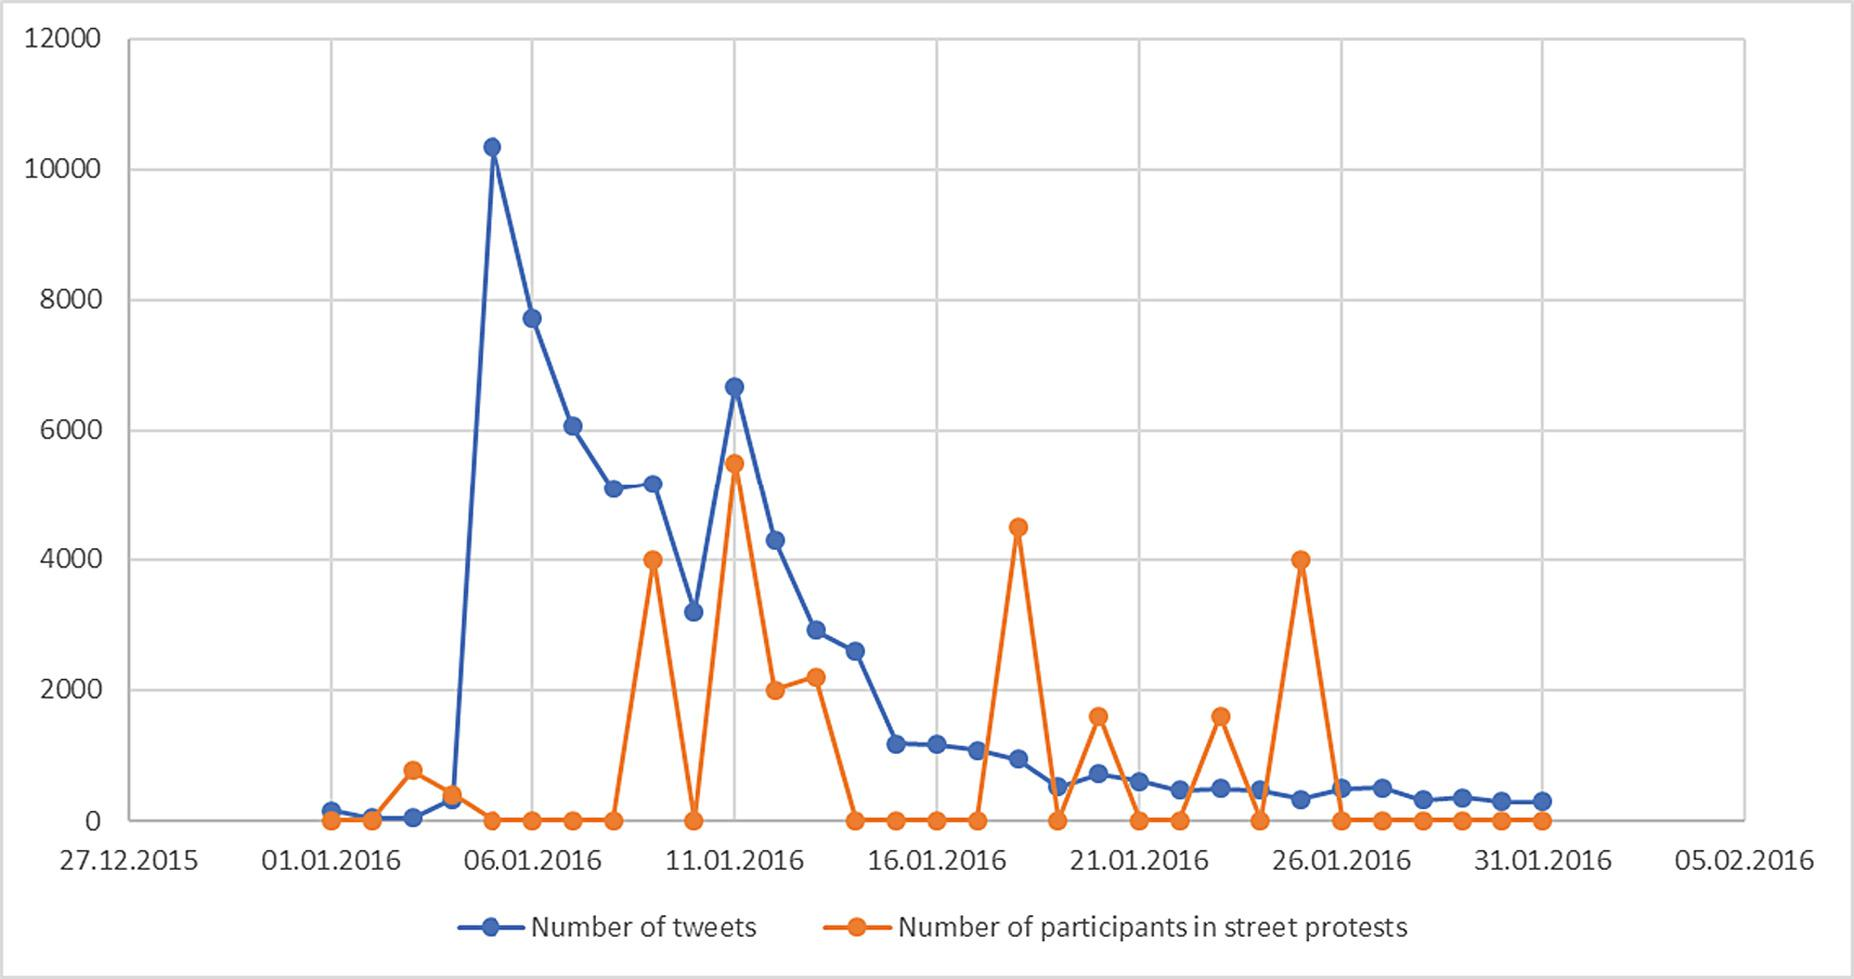
\includegraphics[scale=1.0]{onlineDiscussionTimeSeries}
	}
	\caption{Time series for online discussion and offline events.}\label{fig:onlineDiscussionTimeSeries}
\end{figure}

Granger causality test can statistically determine when one variable precedes and predictively explains another variable \cite{GroshekCloughGroshek} in case when the influence of one 1-dimensional time series parameters \((xt)\) on another time series parameters \((yt)\). The Granger causality analysis are carried out by evaluating of two types of regression:
\[ 
yt = \alpha0 + \alpha1yt - 1 + \ldots + \alpha p yt - p + \beta1xt - 1 + \ldots + \beta1xt - p + \epsilon t
\] and
\[ 
xt = \alpha0 + \alpha1xt - 1 + \ldots + \alpha p xt - p + \beta1yt - 1 + \ldots + \beta1yt - p + \upsilon t
\]
to prove the null hypothesis \(\beta1 = \ldots = \beta p = 0\).

The regressions were carried out in a special program for statistical calculation EViews (Quantitative Micro Software, Version 10). The time lag is set at 2, the level of significance, \(\alpha\), is set at 5\%, We compared two time series -- data with number of participants and data about number of tweets. The null hypothesis about the absence of influence of online activities on the offline activities has been confirmed (Probability = 0,4696), as well as null hypothesis about absence of the opposite causal relation (Probability = 0,8315).

Hence, the idea of causal relationship between street demonstrations and Twitter communication about the event is rejected. Political activities in German cities triggered by New Year’s Eve’s sexual assaults in January 2016 and discussion about them on Twitter demonstrated an asynchronous character and do not depend on each other in the time dynamic.

\subsubsection{4. Detecting Pivotal Points via Topic Modeling}

\paragraph{4.1 The Method}
On the second step of our work with the case, we have tried an alternative methodology to detect patterns of interaction between online and offline activities. Our idea was to trace the change of topicality during the immediate aftermath of the conflict and to see whether the patterns repeat across several cases. In this paper, we look at just one case but we already see a particular pattern in interaction of topicality and protest activity.

To define the pattern, topic modeling was performed on the tweets to model the topic distribution for each day from the period of the study. The algorithm Biterm Topic Model has been chosen due to time restrictions and computational capabilities. BTM has been developed for short texts: this is an efficient algorithm that allows getting coherence topics for short text collections \cite{YanyanJiafengXueqi}.

The BTM algorithm assigns the topics to each document; then, the grouping of the messages and the corresponding topic distribution is performed, whereas the time of publication is used as a criterion for the grouping procedure. After several pre-tests with the number of topics from 20 to 200, 50 topics were chosen to perform the modeling procedure. The list of the topics with distribution coefficients \(p(z)\) for each day of the period has been visualized in a form of a heat map (see Fig.~\cref{fig:topicDistributionJan2016}).

\begin{figure}[ht]
	\centerfloat{
		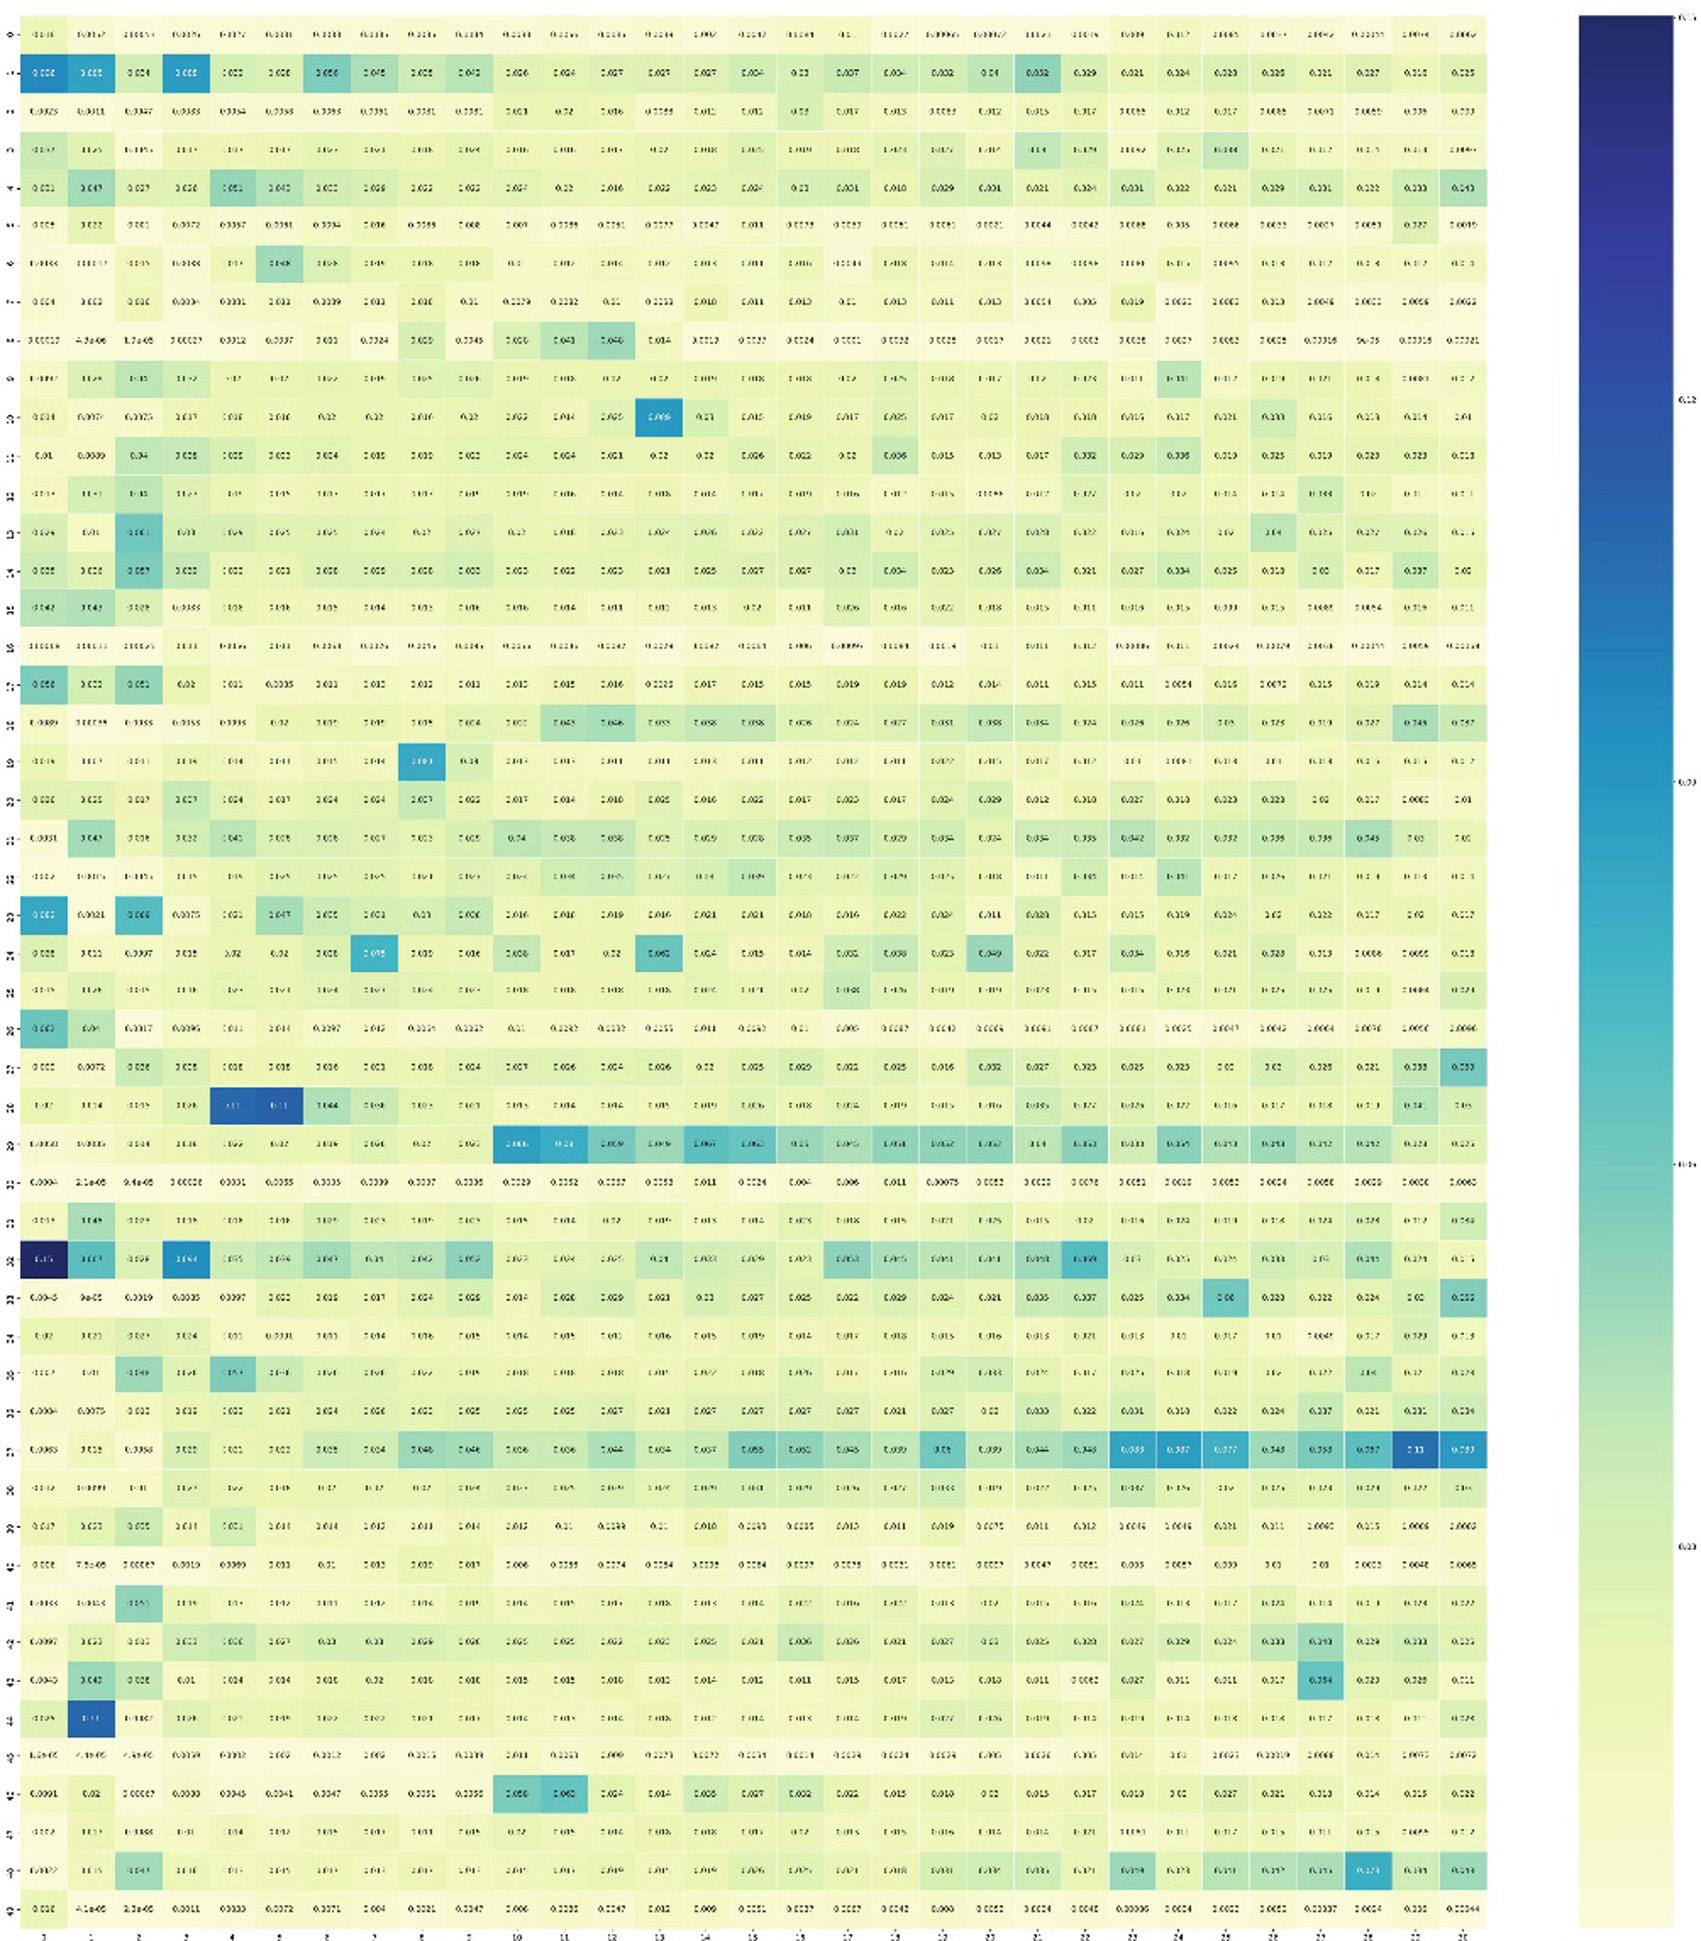
\includegraphics[scale=1.0]{topicDistributionJan2016}
	}
	\caption{Distribution of topics during January 2016 (axis \(x\)) according to their coefficients \(p(z)\) (axis \(y\)).}\label{fig:topicDistributionJan2016}
\end{figure}

To analyze the semantic structure of the discussion, we formed the list of the most salient topics. If the weight of a topic (p) on a particular date exceeded 0,047 (more than 50\% in the daily topic distribution), it indicated that the actuality of this topic has increased sharply. 26 topics that were at particular points more salient than 0,047 are unevenly distributed in the course of January 2016, with most salient topics visible in the first three days of the conflict (five topics on January 1 and 2, six at January 3). In the discussion below, the topics are listed 1 to 50 (instead of 0 to 49 on the heat map).

\subsubsection{5. Results}

As visualized on Fig.~\cref{fig:mostSalientTopicsNYE}, four topics were salient on more than five days during the period of study. Their semantic structure is listed in the Table~\cref{tab:salientTopicsSemanticStructure}. Every topic includes nominations of place, actors, and hashtags employed by the users to frame the issue.

\begin{figure}[ht]
	\centerfloat{
		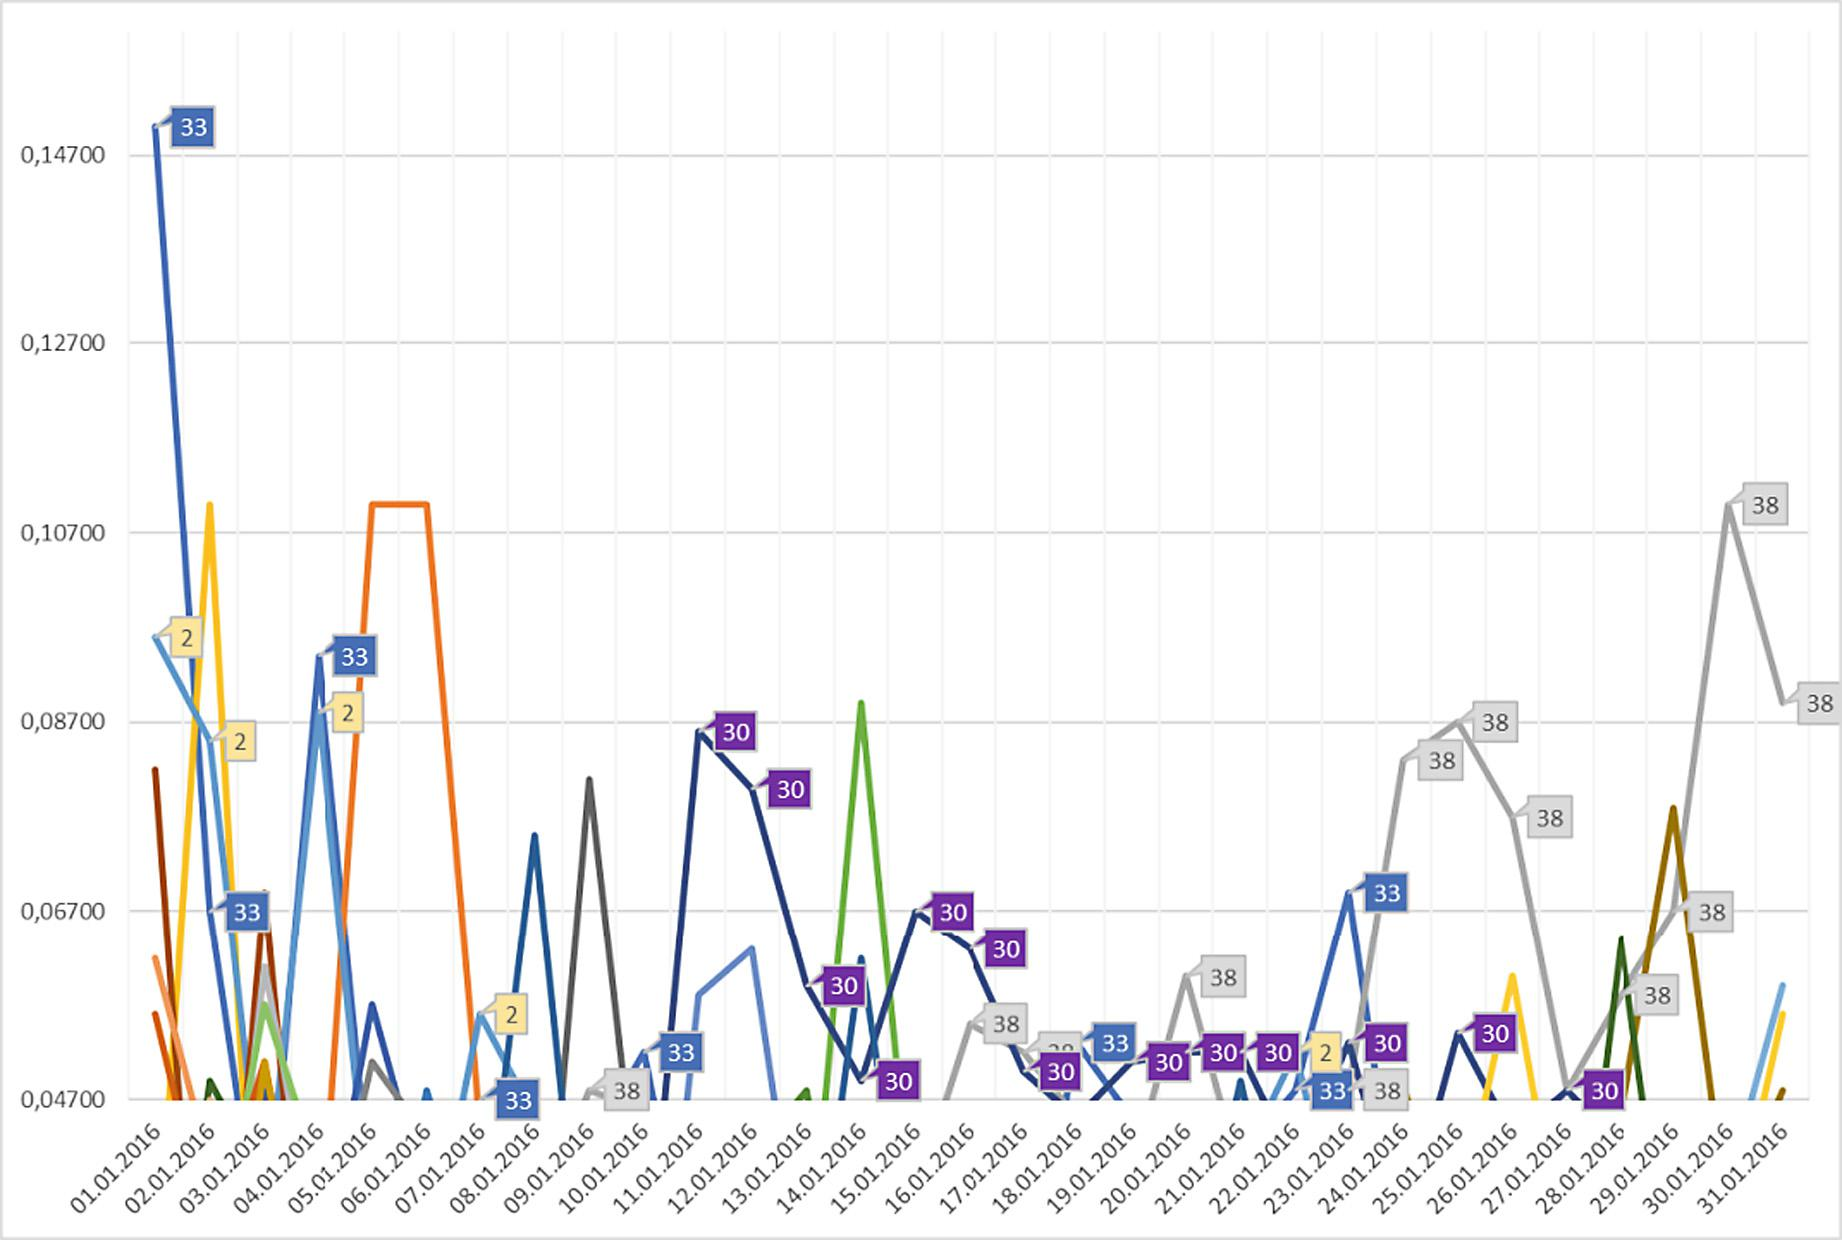
\includegraphics[scale=1.0]{mostSalientTopicsNYE}
	}
	\caption{The most salient topics in the Twitter discussion about New Year’s Eve’s sexual assaults (axis \(y =\) weight of a topic).}\label{fig:mostSalientTopicsNYE}
\end{figure}

\begin{table} [htbp]%
	\centering
	\caption{Semantic structure of the regularly salient topics.}%
	\label{tab:salientTopicsSemanticStructure}% label всегда желательно идти после caption
	\renewcommand{\arraystretch}{1.5}%% Увеличение расстояния между рядами, для улучшения восприятия.
	\begin{SingleSpace}
		\begin{tabulary}{\textwidth}{@{}>{\zz}L >{\zz}C >{\zz}C@{}} %Вертикальные полосы не используются принципиально, как и лишние горизонтальные (допускается по ГОСТ 2.105 пункт 4.4.5) % @{} позволяет прижиматься к краям
			\toprule     %%% верхняя линейка
			Topic N & Top words & Dates of saliency \\
			\midrule %%% тонкий разделитель. Отделяет названия столбцов. Обязателен по ГОСТ 2.105 пункт 4.4.5
			2 &  Ausnahmslos, gewalt, koelnhbf, rassismus, sexualisierte, frauen, sexismus, immer, sexuelle, aufschrei & January 1, 2, 4, 7, 22 \\
			33 &Koelnhbf, ausnahmslos, koeln, muslime, rapefugees, versuch, neue & January 1, 2, 4, 7, 18, 22, 23\\
			30 & Koelnhbf, koeln, polizei, medien, silvesternacht, amp, mueller & January 11 to 17 \\
			38 & Koelnhbf, ausnahmslos, merkel, amp, pegida, schon, mal, abmerkeln, brief & January 19, 20, 21, 23, 25, 27 \\
			\bottomrule %%% нижняя линейка
		\end{tabulary}%
	\end{SingleSpace}
\end{table}

Juxtaposition of the most salient topics clearly shows that there are four periods on the time-series graph when different topics dominated with a varying degree of sal- iency: January 1 to 7; January 8 to 15; January 16 to 23; January 24 to 31 (see Fig.~\cref{fig:topicDistributionPeriods}).

\begin{figure}[ht]
	\centerfloat{
		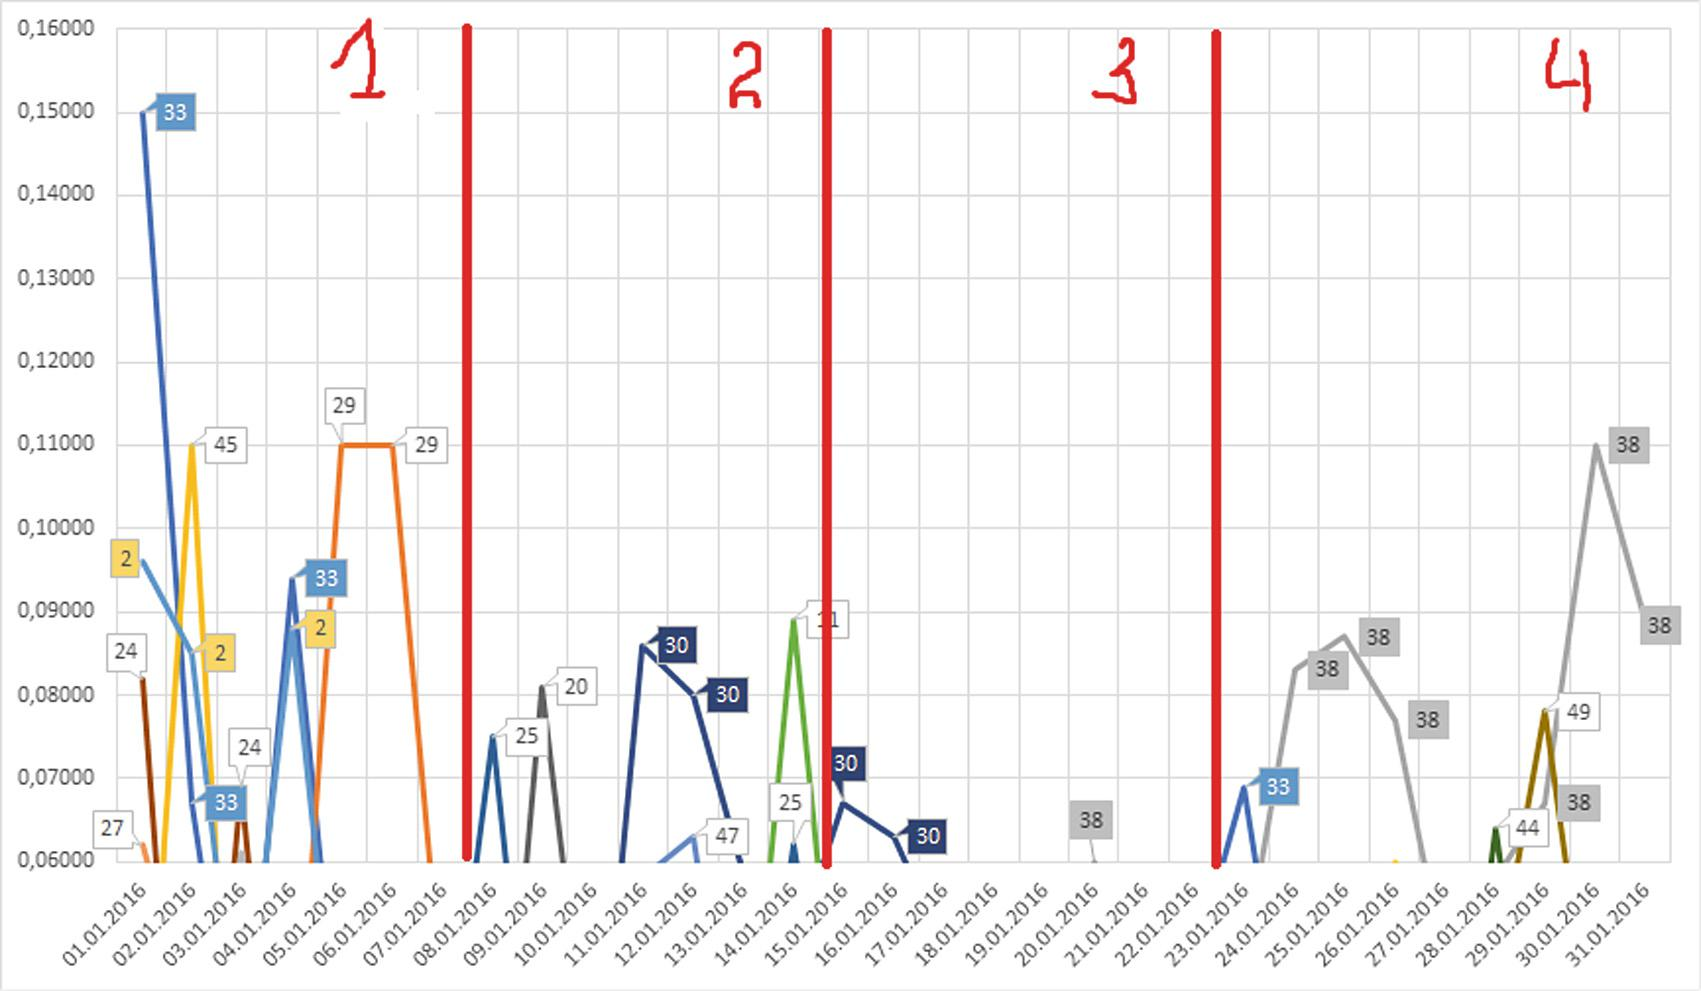
\includegraphics[scale=1.0]{topicDistributionPeriods}
	}
	\caption{Periods in topic distribution.}\label{fig:topicDistributionPeriods}
\end{figure}

In the first period (January 1 to 7, 2016), nominations among the top words define direct participants (topics N2 and N33): women (‘frauen’) against Muslims and ‘rapefugees’. Hashtags \#ausnahmslos and \#aufshrei indicate a feminist voice in the Twitter discussion: the hashtag \#aufschrei was introduced first in 2013 by feminism activist Anne Wizorek. This period was the most ‘buzzy’, according to the number of salient topics.

In the second period (January 8 to 15, 2016), topic N30 is the most salient. It demonstrates the public debate on the role of police and German media during the conflict: both actors were heavily criticized on Twitter. The second most salient topic during one day was the topic N20 that discusses more extensively political authorities who participated in the debate: Minister President of North Rhine-Westphalia Hannelore Kraft, North Rhine-Westphalia’s Interior Minister Ralf Jäger, and North Rhine-Westphalia’s parliamentarian from FDP Christian Lindner.

The third period (January 16 to 21, 2016), as the heat map shows, is a ‘gap’ period between topic N30 that is becoming less salient from its maximum on January 11, and topic N38 that increases in salience tremendously since 24\(^{th}\) of January. According to our time series analysis (see Table~\cref{tab:actionsAndStatementsGermany}), both PEGIDA and NOPEGIDA demonstrations have taken place but the number of tweets reduced significantly from more than 2500 on January 14 to less than 500 on January 23.

Topic N38 dominates the discussion in the last period (January 22 to 31, 2016). It reflects the activity of the PEGIDA movement and its supporters who use the hashtags \#abmerkeln and \#merkelmussweg -- both urge Angel Merkel to leave her Chancellor post.

We tried to trace manually whether the topics relate to the events. Concerning street actions, PEGIDA movement was mentioned only in 3 topics of 50 in our model (N21, N28, N38). Topic N21 goes beyond the saliency threshold only once, on January 2, while the first street action of PEGIDA supporters happened on January 4. Topic N28 passes the salience threshold only once, on January 31, after a wave of street actions. Topic N38 has been most salient before the street protests on January 18 as well as on the days when street actions took place (January 9, 20, 23, and 25). It reaches the highest level of salience (weight of a topic (p) exceeds 0,08) on January 24 and 25 in comparison to \(p = 0,048\) on January 23. In both cases, on January 18 and 25, the biggest number of participants took part in PEGIDA street actions (4000, as estimated by German media reports).

On January 14, Minister President of North Rhine-Westphalia Hannelore Kraft presented the package of actions to be taken for improving security and integration. Salient topics do not mention Kraft and do not relate directly neither to N11 (most salient, \(p = 0,089\), mentions the Head of Cologne’s police Albers fired on January 4 and North Rhine-Westphalia’s Interior Minister Ralf Jäger) nor to N25 (mentions political parties CDU/CSU, AFD, SPD and FDP), nor to N30 (mentions feminist hashtags \#aufschrei and \#ausnahmlos as well as popular hashtag related to the mayor Reker \#einearmlaenge). On the next day, the only topic N30 exceeded the level of \(p > 0,047\). In this case, we do not observe any connection between a political act of authorities and Twitter debate.

\subsubsection{6. Conclusions}

Scholars have tested a wide range of factors influencing political mobilization and, in particular, mass participation in a street action. Internet penetration, online user behavior and participation in online discussions were studied among other parameters. We argue that online behavior cannot be seen is a sole, dominant predictor for spillovers of protest to the street, as scholars that focused on interrelation between online and offline political activities have revealed controversial evidences on the causal relations between them.

In this paper, we presented the pilot study of relations between online and offline political activities triggered by New Year’s Eve’s sexual assaults in Germany 2016. The Granger causality test conducted in a way suggested by authors \cite{BastosMerceaCharperntier}, has failed, partly because the case study is characterized with the lack of parameters and data to compare the level of commitment among Internet users and street actions participants. In such cases, alternative ways to assess the relations between online and offline activities might be needed.

To prove the inter-relation between online discussion and offline political activities, new criteria and parameters are needed to be operationalized. To reveal these parameters for further research, we analyzed the data with the help of topic modelling that has visualized how the topics develop through the online debate.

Based on the results of the topic modeling, we juxtaposed the development of the most salient topics and the timing of the offline political activities in January 2016. Four periods were revealed, including the ‘gap’ period where topic saliency was the lowest. While in two first periods authorities and their (dis)activities were the main focus of the discussion, the fourth period is dominated by the topic that reflects far-right discourse (N38).

Several topics have gone beyond the saliency threshold (weight of a topic \((p)\) exceeding 0,047) before, on, and after the days of street actions; the most visible topics have also reached the highest level of saliency (weight of a topic \((p)\) exceeding 0,08) before the offline events. These intersections should be studied in a more nuanced way, \textit{i.a.} hour by hour. Hence, topic modeling has provided evidence that visibility of political activists precedes the street actions they organize. Moreover, the rapid change of the level of saliency that we observed for the topic N38 took place before the day the biggest number of participants took part in PEGIDA street actions in two cities simultaneously on January 25. If the peak of the topic in an online discussion precedes the mass participation in an offline street action, one might argue that the platform participated actively in forming of protest consensus. Rapid appearance of a peak within a topic, just like we observed for topic N38, might be a predictor for the forthcoming successful mobilization.

We assume that the Granger causality test might provide more accurate results in cases like New Year’s Eve’s sexual assaults in Germany 2016 if the level of street activity is examined against the level of salience of the dominant topics. Significant changes in the level of salience (rapid appearance of a peak with the topic distribution, as observed for topic N38) might be a predictor for the forthcoming successful mobilization. For more conclusions, we will in future compare several case studies of the same nature, to see whether the patterns that we have discovered for Cologne repeats for other countries and cases within Germany.

\section{Методы анализа тональности контента}\label{sec:ch5/sect3}

\subsection{Sentiment analysis for ad hoc discussions using multilingual knowledge-based approach}\label{subsec:ch5/sec3/sub1}

\subsubsection{1. Introduction}

Recently, the number of active users of social networks has increased many times, for example according to the website statista.com: Twitter has 313 million active users per month, 100 million users per day and 500 million tweets are published daily; Facebook has 1.79 billion active users per month, 1.18 billion per day. Such activity also influences people’s reaction to various social, political and economic events in the world. As a result, this means that such events are covered and distributed in social networks several times faster than in other media. Various discussions that arise as a result of any major events have an unpredictable structure of development and a number of specific properties, such as the peculiarity of user interaction among themselves, their relationship to the event, etc. Such discussions are called ad hoc discussions. For example, on Twitter and other social networks on major world events, there are long and branched discussions, the collection and analysis of which is a non-trivial task.

A separate task in the analysis of social networks is to determine the sentiment of the posts of users that were published in the context of any discussion, in particular, in the ad hoc discussion. Sentiment analysis \cite{Liu} is a class of methods that combines algorithms of computer linguistics, semantic and lexical analysis, as well as machine learning. One of the serious problems of analyzing the tonality of texts is the separation of a useful part of the text, that is, one that contains really useful information, and noise -- information that either does not affect the positivity or negativity of the statement, or complicates the precise definition. Another problem that the authors are also trying to solve is the analysis of short texts. So, for example, social network Twitter seriously differs from many other platforms with its limitations on the length of the post, which in 2018 is only 280 characters. This suggests that the messages in in most cases can contain only some essential information, or be spam and noise, detection and screening of which is another task. In addition, another distinctive feature of Twitter is the opportunity to conduct large and branched discussions on certain topics: whether it’s politics, economics, sports, etc., which can be easily monitored using hashtags.

In this paper, taking into account the specifics of short messages on Twitter, the authors set the task to develop a knowledge-based method for sentiment analysis of user messages in two major ad hoc discussions (Ferguson unrest (USA) and Biryuliovo bashings (Russia)). One of the problems that we are trying to solve is the lack of a decent russian lexicon. In fact, there is not one complete and accessible. There have been attempts to create such lexicons, but their effectiveness has not been verified to date. So we create a dictionary of russian affective words and compare its effectiveness with english lexicons.

\subsubsection{2. Current Research in Sentiment Analysis}

Researchers have studied almost all the main aspects of the problem. In their paper \cite{SchullerKnaup}, B. Schuller and T. Knaup propose an approach based on N-Grams and support vector machines \cite{ScholkopfCristianini}, which is very popular among researchers nowadays. In addition, the authors propose an approach that does not require pre-tagged data, and operates on the basis of knowledge-based resources, as well as linguistic analysis. They describe the use of online dictionaries containing both information about words and phrases, and the connections between them. Also, the article considers the possibility of using information about parts of speech of words to improve the accuracy of the analysis results. Also, K. Yessenov \cite{MisailovicYessenov} presented an analysis of the tone of comments to the reviews on films. The authors empirically studied the effectiveness of machine learning algorithms in the classification of text messages to their semantic value. The researchers used comments on the articles on the pop- ular Digg.com resource and investigated them for positivity and negativity. In \cite{RavindranSuchdevKotkar} the authors consider the possibility of combining knowledge-based methods and machine learning algorithms for analyzing users’ messages on the Twitter social network, which differ in their length. In the context of their study, they create a feature vector that contains such information as the number of positive and negative words, emoji and hashtags, and then classify data using machine learning algorithms (in particular, the support vector machine \cite{ScholkopfCristianini}). In addition, the issues of data preprocessing, use of metadata of each tweet and ways of its representation for further classification are considered.

Previous works also described methods for detecting influencers and ordinary users of ad hoc discussions. Often, users with fewer views and likes are more influential than others. This is shown in the articles \cite{BodrunovaLitvinenkoBlekanov2016,BodrunovaLitvinenkoBlekanov2017}, in which users and their connections were presented in the form of graphs and evaluated by various measures of centralities, such as pagerank and betweenness, as well as an expert analysis of the sentiment of users.

There are not many works devoted to the analysis of tonality in Russian. In \cite{BelyatskayaZagibalovCaroll} authors describe comparable corpora of book reviews in English and Russian and present experiments with a sentiment classification system. In \cite{ChetviorkinLoukachevitch} researchers consider a new approach for domain-specific sentiment lexicon extraction in Russian. They propose a set of statistical features and algorithm combination that can discriminate sentiment words in a specific domain. The extraction model is trained in the movie domain and then utilized to other domains.

\subsubsection{3. Proposed Sentiment Analysis Method}

The knowledge-based method developed by the authors includes the following steps:
\begin{enumerate}
	\item Construction of affective dictionaries.
	\item Data preprocessing.
	\item Classification.
\end{enumerate}

\paragraph{3.1 Construction of affective dictionaries} 
To analyze the sentiment of users’ messages in the study of major ad hoc discussions in the social network Twitter authors used a knowledge-based approach based on the construction and application of tagged dictionaries of positive and negative words. These dictionaries were constructed for English, French, Italian, Russian and Spanish languages according to the following principle. The most complete tagged list of English positive and negative words from open sources was selected. In our case, a dictionary that was constructed during the work of the University of Illinois at Chicago staff was used and is being expanded since then \cite{EnglishOpinionWords}. This dictionary contains approximately 6785 words. Initially there were 2005 positive words and 4780 negative words. Further, the procedure of extending the resulting dictionary was applied by adding synonyms from the WordNet database to it as follows. The authors developed a software component that matches each word from the already existing dictionary with a list of synonyms. As a result of the procedure, the dictionary consisted of 5787 and 11660 positive and negative words, respectively. This component checked the extended dictionary for repetitions, and, in case of occurrence of any identical words, deleted them. Using the machine translation procedure, new dictionaries were constructed in the appropriate natural languages. Since the results of the machine translation the repetitions could be formed again, the resulting dictionaries passed the procedure of removing duplicates. As a result of the performed actions, the dictionaries of Russian positive and negative words now consist of 3832 and 3890 words, respectively.

\paragraph{3.2 Preprocessing}
In order to improve the results and improve the accuracy of solving the classification problem, it is first necessary to bring the tweets to a normal view. This process is called normalization and, in addition to bringing all the symbols to the lowercase, includes following three steps.

\textit{3.2.1 Stop-words removal.} First of all, when processing the case, it is necessary to delete all noise words or stop-words. Stop-words are words that are often found in the language and carry almost no semantic meaning. For example, in English, such words can be prepositions (in, on, at, etc.), conjunction (and, but, for, etc.) and other function parts of speech. In addition, numbers, dates and times are also words that are removed from the tweet. In the context of processing tweets, we also remove all the mentions, that are, links to other Twitter users that start with the \@ symbol, as well as all possible links to third-party resources and sites that are not carrying any practically useful information and basically are noise. Since we do not have a tool capable of evaluating the significance of punctuation marks, we also expose them.

\textit{3.2.2 Tokenization.} The next step is to tokenize the text. This means we have to separate the text into significant units (tokens) for further processing. In the case of tweets, the most optimal size of token is one word. Therefore, after the separation, the tweets will be represented by a list of words that remained after the process of stop-words removal.

\textit{3.2.3 Stemming.} The third and final step is stemming \cite{SavoyDolamic}. Stemming is the process of extracting the basis of a word, which in this case may not coincide with the root of the word. In tasks of text classification, stemming is necessary first of all in order to reduce the dimensionality of the problem and increase the productivity of the classifier. There are many stemming algorithms for different languages. The most common is the stemmer of Martin Porter, developed originally only for the English language. But later the main idea of the algorithm was used to create the project "Snowball" and stemmers for different languages. Snowball is a small programming language designed for writing stemming algorithms. In the context of this study, we also subjected the dictionaries constructed in the previous paragraph to the stemming, since in the process of classifying it is necessary to define the polarity of a word, which is fully expressed in its basis.

\paragraph{3.3 Classification}
Our classification algorithm is fed to the input received after a preprocessed list of words that could affect the classification. Each word of this list is checked for the presence in dictionaries of positive and negative words constructed in the previous section. Ultimately, the number of positive and negative words in the list is counted. If the number of positive tokens exceeds zero and the number of negative tokens is zero, then the corresponding tweet is considered as positive, if the number of negative tokens exceeds zero, and the number of positive tokens is zero, then tweet is negative. In all other cases: if these numbers are equal or in some tweet there are both positive and negative tokens, then the tweet is marked as neutral. This approach shows different results on different test cases. This is our first approach.

We also offer a more obvious version of this classifier. In this version, the algorithm is also fed with a list of words obtained after preprocessing, and the number of occurrences of positive and negative words is also considered. However, those tweets whose word lists contain more positive than negative elements are considered positive, tweets that contain more negative than positive words are getting negative tag. Finally, tweet is marked as neutral if numbers of positive and negative words are equal. In this approach, you can see that in most cases tweets will be classified as positive or negative and only a small part of them will be neutral. Because of the fact that in this paper we consider the ad hoc discussion, we propose some adjustment of this algorithm: depending on the topic and features of the current discussions, it is possible to introduce a measure that would allow more precise definition of neutrality of some tweet. In other words, the number of tweets that would be labeled as neutral in the original version of the algorithm would be greater. The proposed metric \(m\) is introduced as follows:
\begin{equation}
	\label{eqn:31}
	m = \frac{p - n}{N}
\end{equation}
where \(p\) is number of positive words in tweet, \(n\) -- of negative words and \(N\) is total number of words in tweet. After the introduction of this metric, you can add to the algorithm some coefficient (let’s say \(c\)), which would be the threshold value for neutral tweets. In other words, if the number of positive and negative words differs slightly, then the tweet is considered neutral. This approach allows you to customize the work of the algorithm, depending on the characteristics of a certain ad hoc debate.

\subsubsection{4. Experiment}
An experiment was conducted to assess the quality of the developed method in three modifications. There were two qualitative measures used: accuracy score and f1 score \cite{Powers}. As a test data there were chosen two real large ad hoc discussions \cite{SmoliarovaBlekanovBodrunova} in Russian and English.

\paragraph{4.1 Test cases description and tagging}
In this paper authors have the opportunity to analyze the data of ad hoc discussions in the social network Twitter of two well-known events: Ferguson unrest (USA) in August 2014 and Biryuliovo bashings (Russia) in October 2013. For each of the events above, there was compiled a list of popular hashtags that describe it:
\begin{enumerate}
	\item Biryuliovo: \#бирюлево, \#мигранты, \#овощебаза, \#зейналов.
	\item Ferguson: \#ferguson.
\end{enumerate}
As a result of the collecting and processing the set of hashtags, we got the following data:
\begin{enumerate}
	\item Biryuliovo: Number of users who have published their tweets in the period since 1st of October 2013 till Thirty-first of October 2013 is 3574. Number of published posts is 10215.
	\item Ferguson: Number of users who have published their tweets in the period since twenty-second of August 2014 till Thirty- first of August 2014 is 70018. Number of published posts is 193812.
\end{enumerate}
On the Figures~\cref{fig:fergusonPublicationActivity} and~\cref{fig:biryulievoPublicationActivity}, one can observe the publication activity of users of discussions about Ferguson and Biryulyovo, respectively. It can be seen that the ad hoc discussions have a different structure: only one "splash" of activity is visible in the discussion of Biryulyovo and the discussion of the situation in Ferguson that has not ceased throughout the week.

\begin{figure}[ht]
	\centerfloat{
		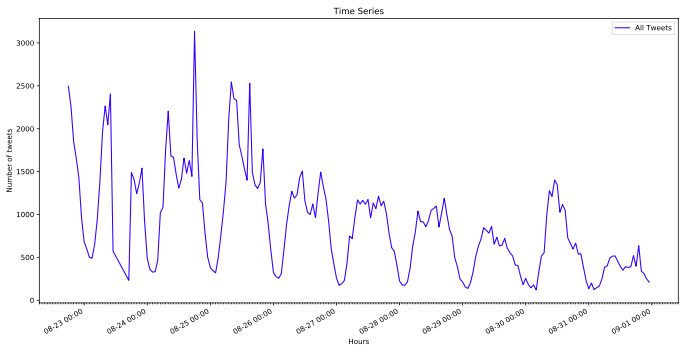
\includegraphics[scale=0.5]{fergusonPublicationActivity}
	}
	\caption{Periods in topic distribution.}\label{fig:fergusonPublicationActivity}
\end{figure}

\begin{figure}[ht]
	\centerfloat{
		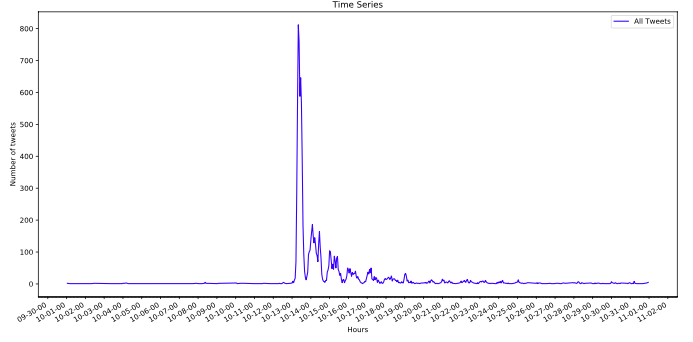
\includegraphics[scale=0.5]{biryulievoPublicationActivity}
	}
	\caption{Periods in topic distribution.}\label{fig:biryulievoPublicationActivity}
\end{figure}

To calculate the qualitaty measures, the authors performed the tagging of the above-described data sets as follows:

\begin{enumerate}
	\item For each ad hoc discussion, lists of top-100 users were compiled according to the number of published messages, as far as betweenness centrality and as far as pagerank centrality \cite{BodrunovaLitvinenkoBlekanov}.
	\item Aggregation of three top-100 lists and deletion of duplicate users. As a result, 213 users were obtained in the Biryuliovo case and 200 in the Ferguson case.
	\item By the aggregated list of users in the Biryuliovo case there were selected all user messages, the total number of which was 3885. In the Ferguson case there were collected just fifteen random messages by each user in order to keep size of the collection slightly equal to the size of Biryuliovo collection.
\end{enumerate}

\paragraph{4.2 Results}
In the course of carrying out the work described above, the problem of the analysis of the ad hoc discussions in the social network Twitter was considered. The authors presented a multi-lingual approach, which is based on the construction and use of affective dictionaries for Russian language and compare it efficiency to expanded existing English lexicon. To assess the quality of the three modifications of this approach, measures accuracy score and f1 score were used on manually annotated data. These results are presented in the Table~\cref{tab:fergusonAccuracyF1}. Results for Biryuliovo case are represented in the Table~\cref{tab:biryliovoAccuracyF1}. These tables show that our best approach gives 0.7 f1 score which is the average result in English \cite{KingHopkins,RavichandranRao}. The results for the Russian dictionaries are slightly lower than the average English. We assume that this is due to the imperfection of machine translation and the difference in the structure of Russian and English.

\begin{table} [htbp]%
	\centering
	\caption{Accuracy and F1 score for Ferguson.}%
	\label{tab:fergusonAccuracyF1}% label всегда желательно идти после caption
	\renewcommand{\arraystretch}{1.5}%% Увеличение расстояния между рядами, для улучшения восприятия.
	\begin{SingleSpace}
		\begin{tabulary}{\textwidth}{@{}>{\zz}L >{\zz}C >{\zz}C >{\zz}C@{}} %Вертикальные полосы не используются принципиально, как и лишние горизонтальные (допускается по ГОСТ 2.105 пункт 4.4.5) % @{} позволяет прижиматься к краям
			\toprule     %%% верхняя линейка
			& First version & Second version & With \(m\) metricy \\
			\midrule %%% тонкий разделитель. Отделяет названия столбцов. Обязателен по ГОСТ 2.105 пункт 4.4.5
			accuracy score  & 0.65 & 0.49 & 0.62\\
			f1 score & 0.70 & 0.52 & 0.66 \\
			\bottomrule %%% нижняя линейка
		\end{tabulary}%
	\end{SingleSpace}
\end{table}

\begin{table} [htbp]%
	\centering
	\caption{Accuracy and F1 score for Biryliovo.}%
	\label{tab:biryliovoAccuracyF1}% label всегда желательно идти после caption
	\renewcommand{\arraystretch}{1.5}%% Увеличение расстояния между рядами, для улучшения восприятия.
	\begin{SingleSpace}
		\begin{tabulary}{\textwidth}{@{}>{\zz}L >{\zz}C >{\zz}C >{\zz}C@{}} %Вертикальные полосы не используются принципиально, как и лишние горизонтальные (допускается по ГОСТ 2.105 пункт 4.4.5) % @{} позволяет прижиматься к краям
			\toprule     %%% верхняя линейка
			& First version & Second version & With \(m\) metricy \\
			\midrule %%% тонкий разделитель. Отделяет названия столбцов. Обязателен по ГОСТ 2.105 пункт 4.4.5
			accuracy score  & 0.57 & 0.41 & 0.55\\
			f1 score & 0.65 & 0.46 & 0.6\\
			\bottomrule %%% нижняя линейка
		\end{tabulary}%
	\end{SingleSpace}
\end{table}

\subsubsection{5. Conclusion}

In this article, authors proposed a multi-lingual approach to the analysis of ad hoc discussions and, in particular, the sentiment analysis of messages in such discussions. The presented algorithms showed quite good results, which were represented in the relevant tables, taking into account the specifics of the given discussions. In the future work, the authors plan to develop this approach and compare it with the work of such classification algorithms as the support vector machines.

\section{Методы суммаризации}\label{sec:ch5/sect4}

\FloatBarrier

